% Options for packages loaded elsewhere
\PassOptionsToPackage{unicode}{hyperref}
\PassOptionsToPackage{hyphens}{url}
%
\documentclass[
  spanish,
]{article}
\usepackage{lmodern}
\usepackage{amsmath}
\usepackage{ifxetex,ifluatex}
\ifnum 0\ifxetex 1\fi\ifluatex 1\fi=0 % if pdftex
  \usepackage[T1]{fontenc}
  \usepackage[utf8]{inputenc}
  \usepackage{textcomp} % provide euro and other symbols
  \usepackage{amssymb}
\else % if luatex or xetex
  \usepackage{unicode-math}
  \defaultfontfeatures{Scale=MatchLowercase}
  \defaultfontfeatures[\rmfamily]{Ligatures=TeX,Scale=1}
\fi
% Use upquote if available, for straight quotes in verbatim environments
\IfFileExists{upquote.sty}{\usepackage{upquote}}{}
\IfFileExists{microtype.sty}{% use microtype if available
  \usepackage[]{microtype}
  \UseMicrotypeSet[protrusion]{basicmath} % disable protrusion for tt fonts
}{}
\makeatletter
\@ifundefined{KOMAClassName}{% if non-KOMA class
  \IfFileExists{parskip.sty}{%
    \usepackage{parskip}
  }{% else
    \setlength{\parindent}{0pt}
    \setlength{\parskip}{6pt plus 2pt minus 1pt}}
}{% if KOMA class
  \KOMAoptions{parskip=half}}
\makeatother
\usepackage{xcolor}
\IfFileExists{xurl.sty}{\usepackage{xurl}}{} % add URL line breaks if available
\IfFileExists{bookmark.sty}{\usepackage{bookmark}}{\usepackage{hyperref}}
\hypersetup{
  pdflang={es},
  hidelinks,
  pdfcreator={LaTeX via pandoc}}
\urlstyle{same} % disable monospaced font for URLs
\usepackage[margin=1in]{geometry}
\usepackage{longtable,booktabs}
\usepackage{calc} % for calculating minipage widths
% Correct order of tables after \paragraph or \subparagraph
\usepackage{etoolbox}
\makeatletter
\patchcmd\longtable{\par}{\if@noskipsec\mbox{}\fi\par}{}{}
\makeatother
% Allow footnotes in longtable head/foot
\IfFileExists{footnotehyper.sty}{\usepackage{footnotehyper}}{\usepackage{footnote}}
\makesavenoteenv{longtable}
\usepackage{graphicx}
\makeatletter
\def\maxwidth{\ifdim\Gin@nat@width>\linewidth\linewidth\else\Gin@nat@width\fi}
\def\maxheight{\ifdim\Gin@nat@height>\textheight\textheight\else\Gin@nat@height\fi}
\makeatother
% Scale images if necessary, so that they will not overflow the page
% margins by default, and it is still possible to overwrite the defaults
% using explicit options in \includegraphics[width, height, ...]{}
\setkeys{Gin}{width=\maxwidth,height=\maxheight,keepaspectratio}
% Set default figure placement to htbp
\makeatletter
\def\fps@figure{htbp}
\makeatother
\setlength{\emergencystretch}{3em} % prevent overfull lines
\providecommand{\tightlist}{%
  \setlength{\itemsep}{0pt}\setlength{\parskip}{0pt}}
\setcounter{secnumdepth}{-\maxdimen} % remove section numbering
\usepackage{draftwatermark}
\SetWatermarkText{Preliminar}
\usepackage{fancyhdr}
\usepackage{graphicx}
\usepackage{parskip}
\usepackage{geometry}
\usepackage{helvet}
\pagestyle{fancy}
\geometry{top=1.5cm, bottom=1cm, left=2.5cm, right=2.5cm}
\renewcommand{\familydefault}{\sfdefault}
\newcommand{\sietepuntos}{\fontsize{7pt}{\baselineskip}\selectfont}
\newcommand{\cincopuntos}{\fontsize{6pt}{\baselineskip}\selectfont}
\addtolength{\headheight}{4.5\baselineskip}
\setlength{\headheight}{70pt}
\setlength{\footskip}{5pt}
\setlength{\textheight}{658pt}
\fancyhead[CO,CE]{
\includegraphics[height=1.5cm]{logoifop.png}\\ \sietepuntos INSTITUTO DE FOMENTO PESQUERO / DIVISION INVESTIGACION PESQUERA}
\fancyhead[LO,LE]{ }
\fancyhead[RO,RE]{ }
\renewcommand{\headrulewidth}{0.5pt}
\fancyfoot[C]{\cincopuntos \thepage \\ \vspace{-0.2cm} ------------------------------------------------------------------------------------------------------------------------------------------------------------------------------------------------------------------------------------------ \\ \vspace{-0.2cm} \cincopuntos CONVENIO DE DESEMPEÑO 2020 IFOP/SUBSECRETARÍA DE ECONOMíA Y EMT \\ \vspace{-0.1cm} INFORME CONSOLIDADO. MERLUZA DEL SUR, 2021}
\ifxetex
  % Load polyglossia as late as possible: uses bidi with RTL langages (e.g. Hebrew, Arabic)
  \usepackage{polyglossia}
  \setmainlanguage[]{spanish}
\else
  \usepackage[shorthands=off,main=spanish]{babel}
\fi
\ifluatex
  \usepackage{selnolig}  % disable illegal ligatures
\fi

\author{}
\date{\vspace{-2.5em}}

\begin{document}

{
\setcounter{tocdepth}{3}
\tableofcontents
}
\textbf{7. ANEXOS}

\textbf{ANEXO I.} Datos y modelo de merluza del sur correspondiente al
modelo consolidado 2020.

\pagebreak

\hypertarget{resumen-ejecutivo}{%
\section{RESUMEN EJECUTIVO}\label{resumen-ejecutivo}}

Este informe se focaliza en la estimación de variables de estado
(e.g.~biomasa desovante) con el propósito de definir el estatus de
explotación de merluza del sur y recomendar un rango de Capturas
biológicamente Aceptables (CBA) para el año 2021. Las variables de
estado fueron estimadas utilizando procedimientos de evaluación de stock
estructurados por edad, los cuales hacen uso de información pesquera,
biológica y de cruceros acústicos para reproducir la dinámica
poblacional etaria de la merluza del sur en la zona sur-austral de
Chile.

La implementación de los procedimientos de evaluación de stock requiere
como primera etapa la actualización de la información pesquera y
biológica disponible. En una base de información definida por flota de
pesca (arrastre industrial, palangre industrial, espinel artesanal),
esta actualización involucró la construcción de índices de abundancia,
series temporales de desembarques, el cálculo de la captura a la edad,
la estimación de biomasa acústica desagregada por edad, y la
construcción de vectores de pesos medios a la edad. Este conjunto de
piezas de información, más parámetros de historia de vida como madurez a
la edad y mortalidad natural, conforman la totalidad de datos empleada
por el procedimiento de evaluación de stock para la estimación de
variables claves para el manejo de la pesquería de merluza del sur.

El procedimiento de evaluación de stock se realiza con información
completa actualizada al 2019 (Mod0\_03a), el proceso envuelve las
siguientes etapas: i) estimación de abundancia poblacional a diciembre
del 2020, ii) cálculo de puntos de referencia biológicos (PBR) basados
en el Rendimiento Máximo Sostenido (RMS), iii) estimación de un rango de
capturas biológicamente aceptables para el año 2021 en base a
ponderadores de la mortalidad por pesca objetivo, y iv) contraste y
consistencia con asesorías previas.

La biomasa desovante, definida como la variable de estado fundamental
para establecer el estado de explotación en merluza del sur, mostró un
leve aumento resultado de la inclusión de los pesos medios anuales de
las flotas y crucero acústico. Los cambios interanuales de la biomasa
desovante dejan ver un agotamiento respecto de la biomasa desovante
virginal de un 31\%. De acuerdo con los objetivos de la administración,
la pesquería de merluza del sur debe tender a un PBR de 40\% de
reducción con respecto a la biomasa desovante virginal. Por lo tanto, el
estado actual de explotación de merluza del sur es clasificado en
sobreexplotación y sobrepesca, pues los niveles de biomasa desovante se
ubican por debajo del PBR objetivo definido como el nivel de biomasa
desovante al rendimiento máximo sostenible (BDRMS), y paralelamente los
niveles de mortalidad por pesca se ubican por sobre el nivel máximo de
mortalidad por pesca objetivo asociada con el rendimiento máximo
sostenible (FRMS).

Por solicitud de la Subsecretaría de Pesca y Acuicultura, se estima una
CBA de tres años para el período 2021-2023. Alcanzando valores promedio
para el período entre 14107 y 19501 toneladas, cuando se aplica una
estrategia de explotación equivalente al FRMS y dependiendo del nivel de
riesgo asumido.

\pagebreak

\hypertarget{objetivos}{%
\section{1. OBJETIVOS}\label{objetivos}}

\hypertarget{objetivo-general}{%
\subsection{1.1. Objetivo general}\label{objetivo-general}}

Estimar la composición, abundancia, biomasa y actualizar el estatus de
los principales recursos pesqueros nacionales e incertidumbre asociada,
proveyendo toda la información y prestando la mejor asesoría a los
Comités Científico Técnicos (CCT) en el análisis de sus posibilidades de
explotación biológicamente sustentables y los niveles de riesgo
involucrados, en un horizonte de corto y mediano plazo.

\hypertarget{objetivos-especuxedficos}{%
\subsection{1.2. Objetivos específicos}\label{objetivos-especuxedficos}}

\begin{enumerate}
\def\labelenumi{\arabic{enumi}.}
\item
  Implementar procedimientos de evaluación de stock basados en
  protocolos científicos para la determinación del estatus de los
  recursos seleccionados, con arreglo al nivel de conocimiento,
  información e incertidumbre correspondiente, conforme a estándares
  actuales en ciencia pesquera.
\item
  Establecer el estatus actualizado de estos recursos, sobre la base de
  sus principales indicadores estandarizados de estado y flujo al menos
  por grupo de pesquerías, incorporando la incertidumbre de estimación
  involucrada, empleando el mejor conocimiento e información disponible
  a la fecha de ejecución del estudio, acorde con los estándares
  definidos por la Subsecretaría de Pesca y Acuicultura y recomendados
  por los Comités Científico Técnicos respectivos.
\item
  Realizar los análisis estocásticos de las posibilidades futuras de
  explotación y la determinación de los niveles de Captura
  Biológicamente Aceptable (CBA) para cada uno de los recursos pesqueros
  considerados en este proyecto, para la siguiente temporada extractiva
  anual (año 2020), reportando el riesgo de no alcanzar los objetivos de
  conservación, considerando la incertidumbre de la estimación de sus
  indicadores y estados probables de la naturaleza , conforme a lo
  dispuesto por la Ley General de Pesca y Acuicultura y el Plan de
  Manejo o Programa de Recuperación respectivo, según corresponda.
\item
  Diseñar y desarrollar evaluación de estrategias de manejo (EEM) para
  las pesquerías de merluza común, merluza del sur y jurel.
\item
  Informar el avance del Programa de Mejoramiento Continuo de la Calidad
  de la de la Asesoría Científica (PMCCAC) realizado durante el presente
  proyecto y consignar en un listado de comprobación (checklist) el
  cumplimiento de cada una de las recomendaciones realizadas en las
  revisiones por pares, cuando corresponda.
\end{enumerate}

\pagebreak

\hypertarget{antecedentes}{%
\section{2. ANTECEDENTES}\label{antecedentes}}

\hypertarget{antecedentes-generales}{%
\subsection{2.1. Antecedentes generales}\label{antecedentes-generales}}

La actividad pesquera en Chile se ha situado como una de las áreas que
ha liderado el crecimiento de la economía nacional. Dicho proceso se ha
basado tanto en los niveles de producción y exportaciones de la pesca
extractiva, así como también, en el rápido desarrollo de la acuicultura.
Por mandato legal, la función pública en la gestión de la actividad
pesquera y de la acuicultura le corresponde a la Subsecretaria de Pesca
y al Ministerio de Economía, Fomento y Turismo, instituciones
responsables de fijar las políticas y establecer las medidas de
regulación que tienen por objetivo conformar el marco legal y normativo
para brindar las condiciones más adecuadas para el desarrollo
sustentable de la actividad de la pesca y la acuicultura. Para cumplir
adecuadamente ese rol resulta esencial contar con fundamentos
científicos y técnicos sólidos en cuanto al conocimiento del estado de
conservación de los recursos biológicos y su ambiente, así como también,
del desempeño de la actividad extractiva.

Con el objeto de atender la misión y sus objetivos estratégicos, desde
1992 la Subsecretaría de Pesca identifica y encarga al Instituto de
Fomento Pesquero (IFOP) ejecutar los programas de seguimiento y
monitoreo de las pesquerías, así como también, la evaluación de stock y
análisis de capturas recomendables para los principales recursos
pesqueros, principal objetivo de la presente investigación.

\hypertarget{antecedentes-de-la-pesqueruxeda}{%
\subsection{2.2. Antecedentes de la
pesquería}\label{antecedentes-de-la-pesqueruxeda}}

La merluza del sur es una especie demersal distribuida en aguas
exteriores e interiores (canales y fiordos) entre la X y XII Región.
Habita entre los 60 y 800 m de profundidad, con las mayores
concentraciones entre los 200 a 400 m. Se encuentra en aguas con
temperaturas entre 3,8ºC y 12ºC (Aguayo 1995), abarcando una
distribución en el cono sur de América que se extiende desde los 36°00'
S en el océano Pacífico suroriental, bordeando el extremo sur de América
para subir hasta los 38°00' S en el lado Atlántico.

El área de operación de la flota dirigida a la captura de merluza del
sur se distribuye entre las latitudes 41°28,6'S a 57°S, en aguas
exteriores (flotas industriales) e interiores (flota artesanal) de la X,
XI y XII Regiones. El área de explotación pesquera se divide en dos
unidades de pesquería, una norte (41° 28,6'S -- 47°S) y otra sur (47°S
-- 57°S), subdivididas en áreas administrativas de aguas interiores y
exterior, teniendo como límite con la zona exterior las líneas de base
recta.

La pesquería de merluza del sur ha operado con clara intencionalidad en
la zona austral de Chile desde el año 1977 y ha sido manejada utilizando
un sistema de Cuota Anual Global de Captura, restricciones al número de
embarcaciones y vedas biológicas, medidas que tienen por objeto evitar o
mitigar los efectos de las actividades pesqueras sobre la especie
objetivo, fauna acompañante y el ecosistema. La magnitud de estas cuotas
surge a partir de las recomendaciones del Instituto de Fomento Pesquero
(IFOP) en base a las estimaciones de abundancia, el potencial productivo
de la población y los niveles de explotación.

Para la evaluación de stock se considera que existe una sola unidad de
stock (Chong y Galleguillos, 1993). Las investigaciones disponibles
señalan que pueden existir diferencias interanuales de algunas semanas
en la fecha de máxima actividad reproductiva, sin embargo, el desove en
merluza del sur alcanza su máxima actividad a fines de invierno. El área
principal de desove se encuentra ubicada entre la isla Guafo (43º37'S) y
la Península de Taitao (47ºS).

La relación de cuotas de captura y desembarques declarados en los años
más recientes es la siguiente:

\hypertarget{revisiuxf3n-de-aspectos-bioluxf3gicos}{%
\subsection{2.3. Revisión de aspectos
biológicos}\label{revisiuxf3n-de-aspectos-bioluxf3gicos}}

El modelo conceptual poblacional de merluza del sur asume que en aguas
chilenas existe un único stock autosustentable distribuido en toda la
zona económica exclusiva. Este supuesto aún es la base de todos los
escenarios de evaluación presentados en la asesoría del año 2014 (Payá,
2015) y ha sido respaldado por el Comité Científico (Quiroz y Wiff,
2012) como también en las reuniones bilaterales IFOP-SUBPESCA
relacionada con la estructura espacial de la población de merluza del
sur (Quiroz et al., 2013).

Antecedentes indican que se identifica una zona única de desove de gran
extensión, además existe información científica que respalda la
existencia de zonas de crianza en aguas interiores de la zona austral,
con mayor preponderancia en los canales y fiordos de la X y XII
Regiones. La distribución de larvas entre aguas interiores y exteriores,
muestra una mayor presencia de larvas de pequeños tamaños en los fiordos
y canales de la zona sur austral, sin detectar mayores diferencias entre
la macrozona norte y macrozona sur .

Se ha descrito un claro patrón migratorio entre aguas interiores y
exteriores, con desplazamientos de la fracción adulta entre macrozonas.
Este patrón de migración estaría confinado principalmente a las aguas
chilenas, con un reducido intercambio de individuos entre éstas y la
plataforma atlántica en el extremo austral de Chile (57°S). Si bien, no
existen antecedentes científicos que posibiliten cuantificar la magnitud
de este intercambio, la dinámica de la pesquería deja ver poco interés
de captura en esta zona del país (rendimientos de pesca reducidos),
sugiriendo que la magnitud de este proceso migratorio debe ser de una
escala muy reducida en comparación con las rutas migratorias con fines
reproductivos.

\hypertarget{estrcutura-poblacional}{%
\subsection{2.3.1 Estrcutura poblacional}\label{estrcutura-poblacional}}

Es posible indicar que el primer estudio sobre unidades poblacionales en
merluza del sur fue realizado por el IFOP en el año 1993, a través de 3
técnicas: marcadores genéticos, análisis de la carga parasitaria y
estudios morfométricos. Para el caso de los marcadores genéticos se
analizaron un total 670 ejemplares, 400 correspondientes a aguas
exteriores y 270 a aguas interiores. Este análisis, realizado a través
de electroforesis de proteínas, mostró que no existen diferencias
significativas en las muestras que provienen de aguas exteriores e
interiores de la PDA (Chong y Galleguillos, 1993). Esto es concordante
con los resultados encontrados a través de la composición y magnitud de
la fauna parasitaria y de la morfometría de merluza del sur, que de la
misma forma indica una alta similitud cualitativa entre las zonas de
pesca. Por otra parte, Chong (1993) utilizó el análisis morfométrico de
estructuras duras (otolitos sagitales), debido a que permite la
discriminación fenotípica entre individuos de diferentes unidades
poblacionales. A través de análisis multivariado de los otolitos, Chong
(1993) concluyo que, si bien las variables morfológicas soportan la
existencia de grupos locales, las variables discriminantes muestran una
importante sobreposición, sugiriendo que los grupos analizados presentan
un alto grado de mezcla, lo que impide considerarlos como unidades
discretas.

En el marco de un estudio FONDEMA ``Diagnóstico merluza del sur y
congrio dorado, aguas Interiores, XII Región'', se desarrollaron
estudios del tipo genético, parasitológico, morfométrico y merístico, a
objeto de determinar la existencia de unidades de stock y poblaciones
residentes de merluza del sur en la XII Región (Daza et al., 2005). Para
verificar la existencia de un stock puro o genético en este estudio se
utilizaron como marcadores moleculares segmentos de ADN mitocondrial
(D-Loop, NADH, Cyt B) y nuclear (Calmodulina e ITS). Los resultados
obtenidos indicaron valores muy bajos de diferenciación genética
poblacional, no permitiendo diferenciar más de un stock de merluza del
sur. Desde la determinación de stocks ecológicos (poblaciones
residentes) por medio de análisis parasitológicos, morfométricos y
merísticos, no se obtuvieron diferencias significativas en la abundancia
de parásitos según el sexo del pez y según la estación temporal.

\hypertarget{mortalidad-natural-crecimiento-y-madurez}{%
\subsection{2.3.2 Mortalidad natural, crecimiento y
madurez}\label{mortalidad-natural-crecimiento-y-madurez}}

Para el modelo de evaluación de sexos combinados, la mortalidad natural
se supone igual a 0.21 y constante a través de los años y las edades. El
modelo implícitamente incorpora el crecimiento en las matrices de
captura a la edad, que como ha sido característico en esta pesquería, no
muestra las fuerzas de las clases anuales o las consecuencias de
explotación severa como la ocurrida entre los años 1986 y 1992, salvo
para los años 2006-2008 donde se observan importantes proporciones de
individuos juveniles de edades entre 4 y 7 años. Los parámetros
biológicos indicados en la Tabla 1 son supuestos constantes en el
modelo.

Tabla 1 Parámetros biológicos a utilizar en el modelo de evaluación. Se
muestra la madurez, mortalidad natural y los pesos a la edad teórico
(dependientes del crecimiento basado en longitud) y empírico (observados
desde la pesquería). Ver sección Pesos Medios para detalles sobre la
utilización de los pesos medios en el modelo de evaluación.

\hypertarget{uxe9poca-y-zona-de-desove}{%
\subsection{2.3.3 Época y zona de
desove}\label{uxe9poca-y-zona-de-desove}}

Los primeros antecedentes de los aspectos reproductivos de merluza del
sur corresponden a observaciones macroscópicas realizadas durante los
años 1977 y 1978 en cruceros de investigación. En estos estudios se
señaló que esta especie desovaría de acuerdo a un esquema similar al de
merluza común, es decir, a fines de primavera y probablemente parte del
verano. En estos cruceros se observaron ejemplares con signos de madurez
a partir de los 70 cm en las hembras y los 59 cm en machos (Avilés y
Aguayo, 1979).

Aguayo et al., (1986, 1987) basado en el análisis del IGS señaló que la
actividad gonádica entre febrero y mayo es leve, para aumentar en
junio-julio y declinar en agosto, lo que indicaría el inicio del desove
masivo. El análisis de los estados de madurez de los ovarios es
coincidente con el comportamiento del IGS. En efecto, Chong (1991)
señaló que la merluza del sur presenta un ciclo de madurez gonádica que
se inicia en febrero y abril con el desarrollo de ovocitos
previtelogénicos y vitelogénicos. Estos últimos son más frecuentes entre
mayo y junio, culminando la madurez y gatillando desoves masivos durante
los meses julio, agosto y septiembre. Aquellos resultados fueron
coincidentes con los reportados por Balbontín y Bravo (1993) y también
con estudios realizados por Aguayo et al., (2001). Las investigaciones
disponibles señalan que pueden existir diferencias interanuales de
algunas semanas en la fecha de máxima actividad reproductiva, sin
embargo, el desove en merluza del sur alcanza su máxima actividad a
fines de invierno.

En cuanto a la zona de desove, Aguayo et al., (2001) señaló que el área
principal de desove en merluza del sur se encuentra ubicada entre la
isla Guafo (43º37'S) y la Península de Taitao (47ºS), foco en el cual se
registran los mayores valores de IGS para el período 1985-1998. Se
registra un núcleo secundario de desove, el cual presenta valores
intermedios de IGS, ubicado entre la Bahía San Pedro (41ºS) y la isla
Guafo (43º37'S).

\hypertarget{migraciones}{%
\subsection{2.3.4 Migraciones}\label{migraciones}}

Hasta el momento, no existen estudios específicos sobre el
comportamiento migratorio de la merluza del sur. Sin embargo, se conocen
antecedentes que se derivan básicamente de la actividad de la flota que
opera sobre este recurso. En este contexto, Aguayo (1995) identificó dos
tipos de migración:

• Migraciones latitudinales, donde se señala que desde julio hasta
octubre de cada año existe una migración gatillada por el desove, donde
los individuos se desplazan desde los centros de abundancia y crianza
hacia la isla Guamblín (44º85 `S). Desde octubre en adelante esta
especie migra hacia el norte, posiblemente en busca de alimento.

• Migraciones longitudinales, donde se observa que a fines de primavera
y comienzos del verano existe una importante migración desde aguas
exteriores hacia aguas interiores. En otoño comienza a desplazarse hacia
aguas exteriores, donde los adultos comenzarían su migración para el
desove que se produce a fines de invierno y principios de primavera.

Las causas de estas migraciones no se conocen a cabalidad, pero
probablemente sea de carácter trófico, asociado a una abundancia
estacional de la sardina de los canales y merluza de cola, como ítems
alimenticios principales.

\hypertarget{zona-de-concentraciuxf3n-de-larvas-y-juveniles}{%
\subsection{2.3.5 Zona de concentración de larvas y
juveniles}\label{zona-de-concentraciuxf3n-de-larvas-y-juveniles}}

Los primeros antecedentes disponibles sobre la distribución de huevos y
larvas de merluza del sur, provienen de un crucero de evaluación del
stock desovante realizado el año 1995 en la zona sur-austral (Lillo et
al., 1996). Este estudio abarcó la zona comprendida entre el norte de la
isla Guafo (43º20'S) hasta cabo Raper (46º20'S). De todas las estaciones
se constató solo un foco significativo de abundancia de larvas situado
al noreste de la isla Guafo. Se señala que el aporte de huevos de
merluza fue escaso con una densidad no mayor a 8 huevos/10 m2 y
mostraron una distribución latitudinal reducida, con presencia entre las
cercanías de Cabo Raper y la isla Garrido (45º12'S).

Por otro lado, Rubilar et al.~(2000), señalaron que la proporción de
ejemplares juveniles en las capturas de merluza del sur en las regiones
X, XI y XII, presenta una clara variación estacional, con aumentos
importantes hacia invierno y primavera. Esta tendencia se refleja en
otros indicadores como la talla y edad promedio en las capturas. En
aguas interiores de la X Región, la mayor presencia de juveniles se
registra en el seno de Reloncaví, destacando la zona de Contao donde la
presencia de juveniles es permanente durante todo el año. En la XI
Región, se observó una dinámica similar, existiendo áreas donde la
proporción de juveniles es permanente durante todo el año como sucede en
el sector comprendido entre la isla Casma a canal Costa. En cuanto a la
XII Región se detecta un aumento de la proporción de juveniles en las
capturas hacia otoño e invierno, pero la proporción es claramente
inferior a lo encontrado en la X y XI Regiones. Resultados similares
para las zonas y épocas de concentración de juveniles fueron reportadas
por Aguayo (1995).

Rubilar et al.~(2000) además señalaron que el aumento de los ejemplares
juveniles de merluza del sur en la captura registrada en las estaciones
en invierno y primavera, sería producto de comportamientos migratorios
de la especie entre aguas exteriores e interiores. En este sentido,
estos autores han planteado la hipótesis referente a que en este período
parte de la fracción adulta de aguas interiores migra hacia aguas
exteriores. Así la población de merluza del sur que permanece en aguas
interiores se caracteriza por una fuerte presencia de juveniles. Esta
hipótesis se encuentra apoyada por las consideraciones realizadas por
Aguayo (1995), por medio de observaciones obtenidas desde los programas
de monitoreo de la pesquería.

\textbf{Ejemplo Nº1: cómo insertar una figura de la carpeta Figuras"}

\begin{center}
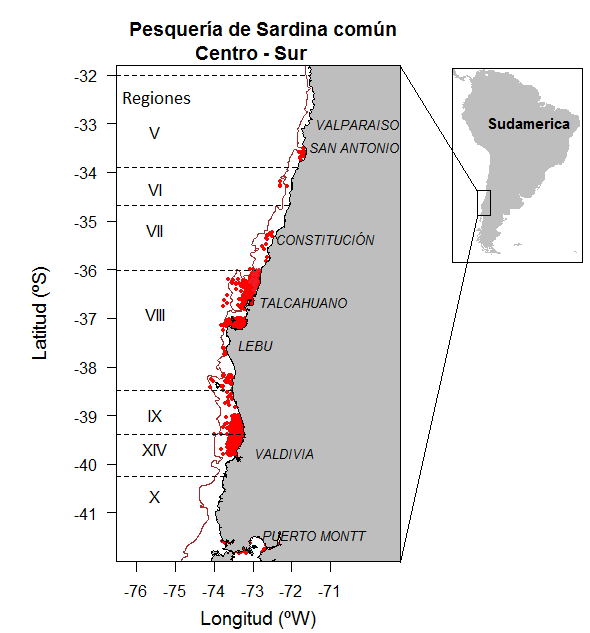
\includegraphics[width=0.8\textwidth]{Figuras/Figura1.png}
\end{center}

\small \textbf{Figura 1}. Distribución espacial de datos provenientes
del muestreo biológico realizado por IFOP para el monitoreo de la
pesquería de sardina común. La línea color café corresponde a la isóbata
de los 200 m. \vspace{0.5cm} \normalsize

\textbf{Ejemplo Nº2: cómo generar un plot y que quede guardado en la
carpeta Figuras}

\begin{center}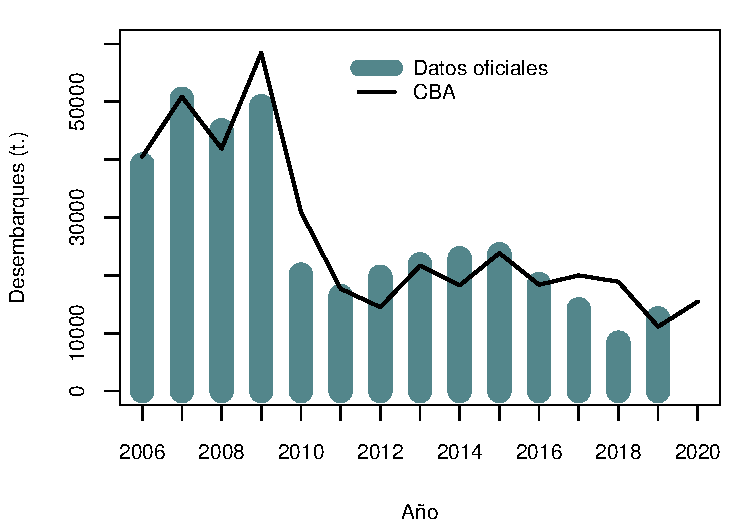
\includegraphics{Figuras/antecedentes_desembarques-1} \end{center}

\pagebreak

\hypertarget{metodologuxeda-de-trabajo}{%
\section{3. METODOLOGÍA DE TRABAJO}\label{metodologuxeda-de-trabajo}}

\hypertarget{objetivo-especuxedfico-1}{%
\subsection{3.1. Objetivo específico
1:}\label{objetivo-especuxedfico-1}}

\emph{``Implementar procedimientos de evaluación de stock basados en
protocolos científicos para la determinación del estatus de merluza del
sur, con arreglo al nivel de conocimiento, información e incertidumbre
correspondiente, conforme a los estándares actuales en ciencia
pesquera.''}

La determinación del estatus de merluza del sur (Merluccius australis)
se basa en la implementación de procedimientos de evaluación de stock
coherentes con del método científico, en el sentido de la implementación
de análisis basados en la mejor información y conocimiento disponible, y
que considera en una amplia dimensión la aplicación del enfoque
precautorio para la pesca establecido por la FAO el año 1996. En este
marco, este objetivo se centra en: i) la descripción de la información
pesquera-biológica y su utilización en el procedimiento de evaluación de
stock, ii) la formulación matemática del modelo de evaluación de stock,
y iii) los métodos estadísticos para evaluar características como bondad
de ajuste, consistencia y pertinencia del procedimiento de evaluación de
stock.

\hypertarget{informaciuxf3n-bioluxf3gico-pesquera}{%
\subsection{3.1.1 Información
biológico-pesquera}\label{informaciuxf3n-bioluxf3gico-pesquera}}

Esta sección se enfoca en la actualización y consolidación de los
antecedentes/datos pesqueros y biológicos disponibles para las unidades
de pesquería de merluza del sur situadas al sur del paralelo 41°28,6 S.
Además, se recaba y compila todos los datos referidos a parámetros de
historia de vida (e.g.~madurez) que permiten sustentar el modelo
conceptual que subyace bajo el modelo de evaluación de stock. La escala
y nivel de agregación espacial y temporal empleada en este estudio, es
definida en coherencia con la información disponible, las
recomendaciones de expertos y los lineamientos definidos por los Comités
Científico Técnicos y la Subsecretaría de Pesca y Acuicultura.
Paralelamente, en esta sección además se describen y actualizan las
estimaciones de biomasa acústica realizadas por las prospecciones
independientes de la pesquería, efectuadas en la zona sur-austral de
Chile.

\begin{enumerate}
\def\labelenumi{\roman{enumi}.}
\tightlist
\item
  Información Pesquera El proceso de evaluación de stock implementado
  incorpora explícitamente tres fuentes de información pesquera:
\end{enumerate}

\begin{enumerate}
\def\labelenumi{\alph{enumi})}
\item
  La primera corresponde a los desembarques reportados en las
  estadísticas oficiales, que representan los niveles de remoción por
  pesca del stock provenientes de las estadísticas oficiales de control
  cuota reguladas por el Servicio Nacional de Pesca y Acuicultura
  (SERNAPESCA). Este sistema de control cuota define la importancia
  relativa de los distintos puertos de descarga y, por lo tanto, es de
  interés administrativo y/o comercial de la actividad. Específicamente
  en esta evaluación, se revisó y actualizo la información de
  desembarques para el periodo 1977-2019.
\item
  Los niveles de descarte y sub-reporte representan la segunda fuente
  pesquera incorporada en el procedimiento de evaluación de stock. Si
  bien, a la fecha no existe un total consenso sobre los métodos y
  niveles de omisión de captura, en la evaluación de stock realizada el
  año 2014 (Payá, 2015) se acordó en el seno del Comité Científico
  Técnico de Recursos Demersales Zona Sur Austral (CCT-RDZSA) utilizar
  un conjunto de ponderadores de descarte/sub-reporte a nivel de flota.
  Basados en estos ponderadores, las series de desembarques anuales
  oficiales fueron corregidas por investigadores de IFOP y
  sensibilizadas en el modelo de evaluación de stock.
\item
  Finalmente, la tercera pieza de información incorporada en el
  procedimiento de evaluación de stock corresponde a los rendimientos de
  pesca desagregados por flota pesquera. Esta información es utilizada
  para la construcción de índices de abundancia derivados de la Captura
  por Unidad de Esfuerzo (CPUE) para las flotas industriales de arrastre
  y palangre, como también, para la construcción de un indicador de tasa
  de captura nominal representativo de la actividad pesquera realizada
  por la flota artesanal.
\end{enumerate}

\begin{enumerate}
\def\labelenumi{\roman{enumi}.}
\setcounter{enumi}{1}
\tightlist
\item
  Información biológica El monitoreo de la pesquería de merluza del sur
  es realizado por el Proyecto de Investigación Situación Pesquerías de
  Peces Demersales y Aguas Profundas, que forma parte del Programa de
  Seguimiento de las Principales Pesquerías Nacionales, estudio
  requerido anualmente por la Subsecretaría de Pesca al Instituto de
  Fomento Pesquero. Este proyecto permite obtener indicadores como las
  estructuras de edad, claves talla-edad, composiciones de tamaños y
  pesos medio a la edad, los cuales conforman el núcleo principal de la
  información biológica empleada en el procedimiento de evaluación de
  stock. En este marco, y con fines de actualizar los datos de entrada
  al modelo de evaluación de stock, se revisaron los siguientes
  indicadores biológicos:
\end{enumerate}

\begin{enumerate}
\def\labelenumi{\alph{enumi})}
\item
  Captura por edad: Denominada también como composición etaria,
  corresponde a la expansión de la captura por flota (arrastre, palangre
  y artesanal), zona (norte y sur del paralelo 47°S) y sexo (machos --
  hembras) mediante una clave edad-talla construida en base a lecturas
  de otolitos recopilados durante la temporada de pesca. La recopilación
  de los otolitos está basada en un diseño de muestreo estratificado por
  clase de tallas, que posibilita construir una matriz de información
  cruzada que representa la distribución de los ejemplares presentes en
  la captura por grupo de edad y por estrato de tamaño. A pesar de que
  se dispone de una estructura de edad por zona, sexo y flota, para
  efecto de la evaluación de stock esta información es agregada por sexo
  y zonas con fines de obtener una estimación global por flota para la
  unidad de pesquería. Esta información es empleada en el proceso de
  evaluación de stock a objeto de evaluar los supuestos de la mortalidad
  por pesca diferenciada por grupos de edad, además de entregar señales
  de la fuerza de las clases anuales que sustentan la fracción vulnerada
  por cada pesquería.
\item
  Pesos a la edad: El crecimiento intra-anual de la merluza del sur es
  recogido en tres matrices de pesos medios a la edad, las que
  corresponden respectivamente a las estimaciones a mitad de año luego
  de la asignación de la edad, calculadas para las flotas de pesca de
  arrastre, palangre, y artesanal, respectivamente. El peso medio es
  empleado para generar las estimaciones de desembarques y biomasa
  vulnerable por cada flota, como también, la biomasa de la acústica
  estimada en agosto de cada año por los cruceros de prospección
  realizados en la zona sur-austral. Al margen de la desagregación de la
  información de pesos medios a la edad, el CCT-RDZSA determinó que la
  asesoría científica basada en el procedimiento de evaluación de stock,
  debe utilizar un vector de peso medio constante a través del tiempo
  que dé continuidad a los supuestos y criterios utilizados en asesorías
  previas. Esto implica que la información de las capturas a la edad y
  abundancia acústica a la edad se unan solo para estimar las
  estructuras, proporcionales a la edad. El cambio de pesos anuales o
  pesos fijos modifica el número de individuos capturados y la
  abundancia a la edad, los cuales ya no son los informados por los
  proyectos de seguimiento y evaluación acústica.
\end{enumerate}

\begin{enumerate}
\def\labelenumi{\roman{enumi}.}
\setcounter{enumi}{2}
\item
  Parámetros de historia de vida Para la implementación del
  procedimiento de evaluación se recoge el conocimiento de estudios
  científicos y técnicos que reportan información asociada a los
  parámetros del ciclo vital de la especie, como la mortalidad natural,
  el crecimiento y madurez. De esta forma, el proyecto tiene un rol de
  integración del conocimiento y utiliza los productos de todos los
  programas y proyectos de investigación para modelar la dinámica del
  recurso.
\item
  Biomasa desovante Acústica La información independiente de la
  pesquería utilizada en la evaluación de merluza del sur corresponde a
  los cruceros acústicos desarrollados durante el período de agregación
  reproductiva. Desde estos cruceros se obtienen las claves talla-edad
  necesarias para generar matrices de abundancia a la edad. Además, los
  cruceros reportan estimaciones de biomasa desovante para el mismo
  período, que para su inclusión en el modelo son considerados como
  valores de biomasa desovante relativa.
\end{enumerate}

\hypertarget{estandarizaciuxf3n-cpue-de-tazas-de-captura-flota-industrial}{%
\subsection{3.1.2 Estandarización CPUE de tazas de captura flota
industrial}\label{estandarizaciuxf3n-cpue-de-tazas-de-captura-flota-industrial}}

Intencionalidad de pesca

La pesquería industrial de merluza del sur ha operado en la zona austral
de Chile (41\texttt{20’S-57}00'S) desde el año 1978. Los reportes de
pesca han dejado ver desde inicios de los 80's una alta concurrencia de
especies en las capturas, las que en algunos años han superado las 100
especies durante la temporada de pesca. Si bien, no más de 5 especies y
grupos taxonómicos (merluza del sur, merluza de cola, congrio dorado,
bacalao y condrictios) representan en promedio el 85\% del total de
desembarques anual, el restante 15\% concurren en diferentes
proporciones dependiendo del tipo de flota y la estacionalidad de las
capturas. En efecto, las proporciones de especies capturadas durante un
lance o viaje de pesca difieren entre tipo de flota; por ejemplo, las
capturas de la flota arrastrera recurrentemente muestran un alto número
de especies como fauna acompañante, aunque la importancia relativa de
estas especies tiende a ser baja, en contraste, la flota palangrera
tiende a capturar un menor número de especies, pero con un número
importante de registros de pesca donde la concurrencia de especies no
objetivo es alta.

Esta dinámica en la flota que captura merluza del sur dificulta la
identificación de la intencionalidad de pesca, requisito indispensable
para el proceso de estandarización de la captura por unidad de esfuerzo
(CPUE). El carácter multiespecífico de las flotas hace necesario
explorar mecanismos o metodologías para la identificación del esfuerzo
de pesca (i.e.~horas de arrastre, días de pesca, numero de anzuelos)
empleado en la captura de una especie objetivo, o más bien, en las
operaciones de pesca con dirección a una especie objetivo. Por lo
anterior, desde el año 2007 el proceso de estandarización de la CPUE en
merluza del sur utiliza el concepto denominado ``táctica de pesca''
(Pelletier y Ferraris, 2000) para clasificar las operaciones de pesca
que son dirigidas a merluza del sur. Utilizando estadística
multivariada, el procedimiento de clasificación de tácticas de pesca
consiste en identificar y agregar las operaciones de pesca que
contienden similitud entre los ensamblajes de especies capturadas a
nivel de lance o viaje de pesca. A este grupo de operaciones le llamamos
``táctica de pesca''. Luego de obtener aquellos grupos de embarcaciones
que definen una táctica de pesca particular, regularmente se examinan
las características espacio-temporales que presenta cada táctica de
pesca. En esta sección se detallan los resultados de la identificación
de tácticas de pesca en merluza del sur.

El procedimiento de estandarización incorpora la táctica de pesca como
un predictor en los modelos lineales de predicción de las tasas de
captura, esto como una vía para aislar los predictores temporales
(Quiroz y Wiff, 2012; Quiroz et al., 2013). Como resumen de la
metodología de estandarización, se implementan 6 etapas donde por medio
de análisis multivariados y modelos lineales es posible diferenciar las
estrategias de pesca que influencian los predictores temporales. Se
realizaron análisis independientes por flota y zonas de pesca dentro de
la zona austral, analizando las bitácoras de pesca que contenían merluza
del sur en sus registros. En el caso de la flota arrastrera, el análisis
abarca desde 1979 a 2019, mientras que en la flota palangrera abarca el
período entre 1987 y 2019.

Las etapas realizadas en este proceso son:

Construcción de matrices con composición de captura para cada lance en
el caso del espinel. Para el arrastre se construyeron matrices con
composición de captura para cada embarcación en un mes determinado en
una subzona determinada. Cada subzona corresponde a medio grado de
latitud. Para cada subzona se acumularon las composiciones de captura
para un barco en un mes determinado.

Análisis de componentes principales (ACP) de la composición de captura,
cuyo objetivo es reducir el total de especies (columnas) en las
componentes ortogonales que representen en su totalidad más del 85\% de
la varianza.

Análisis de Cluster no-jerárquico de los vectores propios derivados del
ACP que cumplían la condición anterior. Este análisis se realizó a
través del método de K-means y como medida de similitud se usó la
distancia euclidiana. Esto permite reducir el número total de registros
(lances de pesca) a 2500 centroides. El uso del cluster no-jerárquico se
debe a que el análisis de dendrograma (cluster jerárquico) es muy
extensivo desde un punto de vista computacional.

Análisis de Cluster jerárquico para construir los dendrogramas de
similitud de los centroides derivados del punto anterior. Se utilizó la
distancia euclidiana y el método de Ward como medida de agrupación entre
las observaciones.

Construcción de los dendrogramas y recuperación de los datos originales
(lances de pesca) para asignarlos a un cluster (táctica de pesca)
determinado.

Estandarización de la CPUE utilizando la táctica de pesca (cluster) como
variables categóricas en un modelo lineal generalizado.

En el caso de la implementación del modelo lineal generalizado, el
primer paso consiste en aplicar un Modelo Aditivo Generalizado (MAG)
usando como variable respuesta a la captura por unidad de esfuerzo y
cuyas variables categóricas pueden ser año, mes y barco, mientras que la
profundidad, latitud y longitud pueden ser asumidas como variables
continuas. Esto permite obtener una aproximación a los coeficientes para
posteriormente incorporar los niveles Cluster (intencionalidad de pesca)
en un predictor de un modelo lineal para la CPUE.

Proceso de estandarización

La captura por unidad de esfuerzo (CPUE) es ampliamente usada como
índice de abundancia relativa en muchas pesquerías del mundo. Las
variaciones de este índice, se asocian principalmente a las
características y composición de la flota, así como a factores de tipo
ambiental. Aquí se presenta la estandarización de las tasas de captura
en la pesquería de merluza del sur, usando la información proveniente de
las bitácoras de pesca entre los años 1979 y 2019 para el arrastre, 1987
a 2019 para palangre. Se utilizaron modelos lineales generalizados
(MLG), técnica que ha sido el método más utilizado en la estandarización
de CPUE (Punt et al., 2000). Este método permite realizar interacciones
entre las variables explicatorias en la CPUE, así como explorar
distintas distribuciones de error mediante la utilización de la
verosimilitud en el ajuste del modelo (McCullagh y Nelder, 1989). Bajo
este enfoque, el modelo general para la determinación de la CPUE es:

donde, es el intercepto, son los coeficientes que dan cuenta de la
variación en la CPUE con respecto al predictor y es un error normal con
media 0 y varianza constante . Los factores analizados para el caso de
la pesquería de arrastre y espinel fueron: años, meses, barco
(aleatorio), zona (unidad de pesquería) y cluster. El efecto cluster
corresponde a la táctica de pesca y se representa en las bitácoras de
pesca por medio de una ``etiqueta'' que lleva cada lance de acuerdo al
cluster donde se ha agrupado la operación de pesca.

La CPUE anual es función de tres variables estimadas a través de MLG:

donde, es el coeficiente estimado para el año i, es el intercepto del
modelo (media global o referencial) y representa el parámetro de
dispersión de la distribución asumida para el error.

\hypertarget{modelo-de-evaluaciuxf3n-de-stock}{%
\subsection{3.1.3 Modelo de evaluación de
stock}\label{modelo-de-evaluaciuxf3n-de-stock}}

La evaluación de stock en Chile ha sido desarrollada y perfeccionada por
IFOP durante los últimos 15 años y cuya metodología se encuentra en
general acorde con los estándares internacionales vigentes. Como una vía
para mantener este estándar, también se han incorporado las
recomendaciones emanadas tanto desde los Comités Científico Técnicos
como de los lineamientos entregados por el equipo de expertos
internacionales en el marco del proyecto ``Revisión de los puntos
biológicos de referencia (Rendimiento Máximo Sostenido) en las
pesquerías nacionales'' (Payá et al., 2014).

El modelo poblacional de merluza del sur asume que en aguas chilenas
existe un único stock autosustentable distribuido en toda la zona
económica exclusiva. El ciclo anual del modelo comienza con el ingreso
de nuevos reclutas de edad 1 (a inicios de año) que dependen de un único
stock desovante. No se consideran procesos de migración/inmigración. Se
implementa un modelo que asume error de observación en las capturas
utilizando la ecuación de Baranov y donde las mortalidades por pesca son
estimadas como parámetros en el modelo. Las biomasas son calibradas
utilizando series de abundancia relativas basadas en CPUE y estimaciones
de cruceros acústicos.

Durante la implementación del modelo poblacional de merluza del sur, se
consideran elementos de incertidumbre estructural basados en el nivel de
conocimiento y de la información o datos disponible, así como la
incertidumbre de estimación generada de su aplicación al conjunto de
datos disponibles. En este sentido, el modelo de evaluación de stock de
merluza del sur se basa en el análisis estadístico de la dinámica de
estructuras de edad anual y pesos medios a la edad, por medio de los
siguientes componentes:

Condiciones Iniciales

Se asume que la población de merluza del sur al comienzo del año 1977 se
encontraba en una condición de equilibrio libre de pesca. Bajo este
supuesto, el reclutamiento del año 1977 corresponde a un reclutamiento
virginal (Ro) consistente con una biomasa desovante virginal (So),
mientras que en posteriores años (\textgreater1977) es dependiente de
una relación stock-recluta Beverton-Holt (función de la BD, Bo, Ro y h)
perturbada por desviaciones obtenidas desde una distribución de
probabilidad normal. Si bien, este supuesto simplifica la estructura del
modelo, es un escenario altamente probable para la población de merluza
del sur. De esta forma, el número de ejemplares de edad a, al comienzo
del año 1977 es definida como,

La biomasa desovante virginal (en número) es obtenida como,

donde y corresponden a la proporción de hembras maduras y pesos medios a
la edad a, respectivamente.

Reclutamiento

Con objeto de estimar los reclutamientos (especificados a la edad 1), se
utilizó el modelo stock-recluta de Beverton-Holt con una estructura de
error lognormal, que incorpora un término de varianza que soslaya el
sesgo durante la trasformación a escala real,

donde es la biomasa desovante en el año t, es la desviación del
reclutamiento en el año t, y es la desviación estándar de las
desviaciones del reclutamiento en escala logarítmica. La relación entre
los niveles virginales de reclutamiento y abundancia desovante, y los
parámetros a y b del modelo Beverton-Holt es dada por,

donde h es un parámetro que define la fuerza de la densodependencia, es
la biomasa desovante virginal, y es el reclutamiento promedio producido
cuando la poblacional se encontraba en equilibrio libre de pesca
(reclutamiento virginal). El término h, definido como el parámetro de
escarpamiento, representa el nivel de reclutamiento relativo al
reclutamiento virginal, que ocurre cuando la biomasa desovante ha sido
reducida a un 20\% de su nivel virginal. Al igual que en la última
evaluación se supuso h igual a 0,5. Como base estructural se continúa
utilizando la biomasa desovante como predictor de los reclutamientos,
que y es calculada en septiembre de cada año por la siguiente expresión:

Evolución temporal de cohortes

La abundancia de merluza del sur a la edad a al tiempo t, es modelada
por

tal que,

donde M es la tasa instantánea de mortalidad natural para la edad a al
tiempo t, m es el grupo plus y Z\_(a,t) es la mortalidad total
edad-específica. En este sentido, se plantea que la dinámica poblacional
de la abundancia N\_(a,t) a la edad a al tiempo t, puede ser
representada por un modelo de sobrevivencia donde las mortalidades por
pesca anuales, F\_t\^{}g, para cada flota de pesca g, son aplicadas en
forma continua durante la estación de pesca para cada edad a de acuerdo
a una ojiva de selectividad S\_a\^{}g.

Selectividades

La curva de selectividad implementada en el modelo para las flotas
arrastre, espinelera y palangrera, como también en los cruceros,
corresponde a una función doble-normal definida para todo el rango de
edad. La función doble-normal utiliza tres parámetros, la edad máxima de
selectividad (k) y las varianzas del lado derecho e izquierdo de la
curva. Estos tres parámetros otorgan considerable flexibilidad a la
funcionalidad de la selectividad, definida como,

La curva de selectividad es asintótica cuando la varianza derecha tiene
a valores altos y conforma una curva tipo domo cuando adopta valores
bajos. Se considera constante entre años tanto a nivel de parámetros de
posición (edad al 50\% de explotación) como de dispersión (pendiente de
la curvatura). Las justificaciones para este supuesto se basan en la
poca variabilidad que presentan las composiciones de edades de las
capturas y en menor grado en los cruceros, como también a que en esta
pesquería no se conocen procesos de escape significativos de individuos
longevos fuera de la zona donde opera la pesquería en el caso de curvas
de selectividad asintóticas.

Valores Predichos

Los índices anuales de abundancia relativa para cada flota g, incluyendo
las estimaciones de los cruceros hidroacústicos, se asumen proporcional
a la biomasa vulnerable estimada a mitad del año, según,

donde q\_g corresponde al coeficiente de capturabilidad de cada uno de
los artes o aparejos de pesca.

En el caso de los cruceros acústicos, se asume que las estimaciones
representan una fracción de la biomasa desovante disponible, lo que en
otras palabras se traduce en que el índice de proporcionalidad o
capturabilidad es estimado en el modelo sujeto a una distribución a
priori, establecida siguiendo una distribución lognormal con media 0 y
error estándar 0,4. Lo anterior se justifica dado que el proceso de
agregación de la merluza del sur posiblemente es más extendido que el
tiempo prospectado, de manera que el crucero admite un coeficiente de
variación de 40\% en términos de la precisión de estimación.

La proporción de edad observada de las flotas de pesca y los cruceros (p
donde C\_(a,t)\^{}g corresponde a la matriz de captura a la edad
observada de la flota g, mientras que N\_(a,t)\^{}g corresponde a la
abundancia a la edad estimada en los cruceros acústicos.

El desembarque anual por flota, , es modelado asumiendo un error de
observación en el proceso de pesca, de esta forma, los desembarques son
estimados como:

Las capturas totales incorporadas en el modelo, corresponden a los
niveles de desembarques anuales realizados por las flotas de pesca
industrial (arrastre y palangre) y artesanal (espinel). Bondad de ajuste
y consistencia del modelo de evaluación de stock Con el fin de asegurar
la aplicación del mejor modelo de evaluación, así como su pertinencia,
consistencia e incertidumbre resultante, se consideró los siguientes
procedimientos:

Se prueba la consistencia de la evaluación mediante análisis
retrospectivos, sobre la base del mismo conjunto de datos empleados.

Se presenta gráficamente el ajuste del modelo a los datos y la bondad de
ajuste de los diferentes modelos empleados, cuando corresponda. Lo
anterior se acompañará con análisis de residuales de las principales
fuentes de datos.

Se incluye la comparación de resultados con versiones anteriores u otros
modelos para evaluar la consistencia de la evaluación presente (análisis
retrospectivo empírico).

Sobre la base de estos análisis, se identifica las oportunidades de
mejoras en la implementación del procedimiento de evaluación, los vacíos
de conocimiento y de información, entre otros.

\hypertarget{anuxe1lisis-retrospectivo}{%
\subsection{3.1.4 Análisis
retrospectivo}\label{anuxe1lisis-retrospectivo}}

Mohn (1999), describe el análisis retrospectivo como una incoherencia
sistemática entre una serie de estimaciones del tamaño de la población o
las variables involucradas en la evaluación, relacionado con series de
información cada vez mayores. Los patrones retrospectivos pueden ser
causados por una serie de factores, pero todos requieren un cambio en el
valor del parámetro o valor del modelo asumido en el tiempo. Las tres
principales causas que provocarían los patrones retrospectivos son: los
cambios en el nivel de las capturas en la evaluación, los cambios en la
tasa de mortalidad natural (M), o cambios en la capturabilidad (q)
(Legault, 2009).

El estadístico rho de Mohn (1999) se ha utilizado comúnmente para medir
el patrón retrospectivo y se define como la suma de la diferencia
relativa entre una cantidad estimada a partir de una evaluación con una
serie de tiempo reducida y la misma cantidad estimada a partir de la
serie de tiempo completa.

Donde X denota alguna variable de la evaluación de stock como F o SSB, y
denota el año, npeels expresa el número de años que se eliminan de forma
sucesiva y la repetición de la evaluación, Y es el último año en la
serie de tiempo completo, tip muestra la estimación terminal de una
evaluación con una serie de tiempo reducida, y ref indica la evaluación
utilizando la serie de tiempo completa.

Este cálculo será cero cuando las evaluaciones reducidas coincidan
exactamente con la evaluación completa o cuando las diferencias entre
las evaluaciones limitadas y evaluación completa están equilibradas
tanto positivas como negativamente. El primer caso no tiene el cambio de
año en año, mientras que el segundo caso se caracteriza por exhibir el
ruido, pero no un patrón retrospectivo. El valor de rho será grande, ya
sea positivo o negativo, cuando hay un patrón consistente de cambio en
las evaluaciones reducidas relativo a la evaluación de series de tiempo
completa.

Para desarrollar este análisis, se utilizó la eliminación sistemática de
datos del año terminal de forma secuencial durante cinco años en
relación al modelo. Este análisis, por lo tanto, permite evaluar la
incertidumbre del modelo mod0\_03 y mod0\_03b, a la estimación de la
biomasa desovante, el reclutamiento y la mortalidad por pesca a los
resultados del análisis retrospectivo.

\textbf{Ejemplo Nº3 cómo incorporar una tabla con formulas}

\textbf{Algunos ayuda memoria para escribir ecuaciones en latex :}

\url{http://minisconlatex.blogspot.com/2010/11/ecuaciones.html}

\url{https://manualdelatex.com/tutoriales/ecuaciones}

\url{https://rinconmatematico.com/instructivolatex/formulas.htm}

\small
\begin{center} 
\textbf{Tabla 4.}
\end{center}
\begin{center} 
\vspace{-0.2cm} Modelo de las observaciones del Modelo Anual con información en tallas.
\end{center}

\begin{longtable}[]{@{}lll@{}}
\toprule
\begin{minipage}[b]{(\columnwidth - 2\tabcolsep) * \real{0.21}}\raggedright
Variable\strut
\end{minipage} &
\begin{minipage}[b]{(\columnwidth - 2\tabcolsep) * \real{0.40}}\raggedright
Ecuación\strut
\end{minipage} &
\begin{minipage}[b]{(\columnwidth - 2\tabcolsep) * \real{0.39}}\raggedright
Descripción\strut
\end{minipage}\tabularnewline
\midrule
\endhead
\begin{minipage}[t]{(\columnwidth - 2\tabcolsep) * \real{0.21}}\raggedright
Captura estimada en número a la edad\strut
\end{minipage} &
\begin{minipage}[t]{(\columnwidth - 2\tabcolsep) * \real{0.40}}\raggedright
\(\hat{C}_{l,t}=\frac{F_{l,t}}{Z_{l,t}}N_{l,t}\left(1-S_{l,t}\right)\)\strut
\end{minipage} &
\begin{minipage}[t]{(\columnwidth - 2\tabcolsep) * \real{0.39}}\raggedright
\(\hat{C}_{l,t}\) Captura en número estimada a la longitud \emph{l}

y \emph{t} en el año.\strut
\end{minipage}\tabularnewline
\begin{minipage}[t]{(\columnwidth - 2\tabcolsep) * \real{0.21}}\raggedright
Desembarques en peso\strut
\end{minipage} &
\begin{minipage}[t]{(\columnwidth - 2\tabcolsep) * \real{0.40}}\raggedright
\(\hat{Y}_t=\sum_l \hat{C}_{l,t}w_{l}\)\strut
\end{minipage} &
\begin{minipage}[t]{(\columnwidth - 2\tabcolsep) * \real{0.39}}\raggedright
\(w_{l}\) es el peso medio a la longitud \emph{l}\strut
\end{minipage}\tabularnewline
\begin{minipage}[t]{(\columnwidth - 2\tabcolsep) * \real{0.21}}\raggedright
Proporción de la captura a la longitud de la flota\strut
\end{minipage} &
\begin{minipage}[t]{(\columnwidth - 2\tabcolsep) * \real{0.40}}\raggedright
\(\hat{p}^f_{l,t}=\frac{\hat{C}_{l,t}}{\sum_l\hat{C}_{l,t}}\)\strut
\end{minipage} &
\begin{minipage}[t]{(\columnwidth - 2\tabcolsep) * \real{0.39}}\raggedright
\(\hat{C}_{l,t}\) Captura en número estimada a la longitud
\emph{l}.\strut
\end{minipage}\tabularnewline
\begin{minipage}[t]{(\columnwidth - 2\tabcolsep) * \real{0.21}}\raggedright
Abundancia a la longitud del crucero\strut
\end{minipage} &
\begin{minipage}[t]{(\columnwidth - 2\tabcolsep) * \real{0.40}}\raggedright
\(\hat{N}_{l,t}^c=N_{l,t} e^{-dt^cZ_{l,t}}S^c_l\)\strut
\end{minipage} &
\begin{minipage}[t]{(\columnwidth - 2\tabcolsep) * \real{0.39}}\raggedright
\(dt^c\) es la fracción del año en la cual se realiza el crucero\strut
\end{minipage}\tabularnewline
\begin{minipage}[t]{(\columnwidth - 2\tabcolsep) * \real{0.21}}\raggedright
Selectividad del crucero\strut
\end{minipage} &
\begin{minipage}[t]{(\columnwidth - 2\tabcolsep) * \real{0.40}}\raggedright
\(S_l^c=\left(1+exp\left[-ln19\frac{(l-l_{50\%}^c}{\Delta^c}\right]\right)^{-1}\)\strut
\end{minipage} &
\begin{minipage}[t]{(\columnwidth - 2\tabcolsep) * \real{0.39}}\raggedright
\(l_{50\%}^c\) longitud al 50\%

\(\Delta^c\) rango entre la longitud al 95\% y 50\%\strut
\end{minipage}\tabularnewline
\begin{minipage}[t]{(\columnwidth - 2\tabcolsep) * \real{0.21}}\raggedright
Biomasa total del crucero\strut
\end{minipage} &
\begin{minipage}[t]{(\columnwidth - 2\tabcolsep) * \real{0.40}}\raggedright
\(\hat{B}_t^c=q^c\sum_l\hat{N}_{l,t}^{c}w_l\)\strut
\end{minipage} &
\begin{minipage}[t]{(\columnwidth - 2\tabcolsep) * \real{0.39}}\raggedright
\(w_{l}\) es el peso medio a la longitud \(q^c\) es la capturabilidad/
disponibilidad del crucero\strut
\end{minipage}\tabularnewline
\begin{minipage}[t]{(\columnwidth - 2\tabcolsep) * \real{0.21}}\raggedright
Captura por Unidad de esfuerzo\strut
\end{minipage} &
\begin{minipage}[t]{(\columnwidth - 2\tabcolsep) * \real{0.40}}\raggedright
\(\hat{CPUE}_t=q\left[\sum^{lmax}_{lmin}S_{l,t}N_{l,t}w_l\frac{(1-exp(-Z_{l,t}))}{Z_{l,t}}\right]\)\strut
\end{minipage} &
\begin{minipage}[t]{(\columnwidth - 2\tabcolsep) * \real{0.39}}\raggedright
\emph{q}: coeficiente de capturabilidad\strut
\end{minipage}\tabularnewline
\bottomrule
\end{longtable}

\pagebreak

\hypertarget{objetivo-especuxedfico-2}{%
\subsection{3.2. Objetivo específico
2:}\label{objetivo-especuxedfico-2}}

\emph{``Determinar las variables poblacionales de los recursos pesqueros
en estudio conforme al marco legal vigente y estimar el valor de los
Puntos Biológicos de Referencia, determinados por los Comités Científico
y Técnicos (CCT) respectivos, bajo condiciones de incertidumbre
estructural y de estimación empleando el mejor conocimiento e
información disponible a la fecha de ejecución del estudio.''}

\hypertarget{definiciuxf3n-de-estatus}{%
\subsection{3.2.1 Definición de
estatus}\label{definiciuxf3n-de-estatus}}

El estado de explotación de la merluza del sur se establece en base a la
posición relativa de la biomasa desovante y mortalidad por pesca con
respecto a los Puntos Biológicos de Referencia (PBR) basados en el
Rendimiento Máximo Sostenido (RMS). Por lo tanto, Las variables de
estado como la biomasa desovante (o adulta), reclutamientos y mortalidad
por pesca, son parte del conjunto de resultados que en primera instancia
emana desde el proceso de evaluación de stock. En este mismo proceso son
estimados los niveles de incertidumbre para las variables de estado
relevantes que definen el estado de explotación de merluza del sur.

En el contexto de la Ley General de Pesca y Acuicultura (LGPA) se
establece que las pesquerías deberán alcanzar o mantenerse en torno del
RMS considerando las características biológicas de los recursos
explotados. El RMS se produce cuando el stock desovante se reduce
notablemente antes que el reclutamiento se vea impactado, para lo cual
requiere estimar los siguientes PBRs:

\begin{itemize}
\tightlist
\item
  Biomasa desovante en el Rendimiento Máximo Sostenible (BDRMS), bajo la
  cual el recurso califica en sobreexplotación.
\item
  Mortalidad por Pesca en el Rendimiento Máximo Sostenible (FRMS), sobre
  la cual el recurso califica en sobreexplotación.
\item
  Biomasa desovante límite (BLIM) bajo la cual una pesquería califica de
  agotada o colapsada.
\item
  Mortalidad por Pesca límite (FLIM) a partir de la cual el recurso
  califica en sobrepesca.
\end{itemize}

La estimación de estos PBRs se basa en el Marco Biológico de Referencia
establecido por el CCT-RDZSA y la determinación de Puntos Biológicos de
Referencia (PBR).

\hypertarget{puntos-bioluxf3gicos-de-referencia}{%
\subsection{3.2.2 Puntos Biológicos de
Referencia}\label{puntos-bioluxf3gicos-de-referencia}}

Durante el año 2014, el Instituto de Fomento Pesquero implementó un
Sistema de Niveles (conocido en la literatura pesquera como Tiers
System), donde cada stock explotado no solamente fue clasificado de
acuerdo a la calidad y cantidad de información disponible para
propósitos de la evaluación de stock, sino también, en base a los
métodos de evaluación más plausibles que podrían ser implementados con
los datos disponibles (Figura 1).

En el caso de la merluza del sur existe una gran cantidad de información
disponible para realizar la evaluación de stock, concurren índices de
abundancia para cada flota comercial, como también, un crucero acústico
que abarca un periodo de 15 años. Además, existe información edad
estructurada para un período de más de 20 años en cada flota. La
evaluación consiste en un modelo de evaluación estándar estructurado a
la edad que utiliza una relación stock recluta Beverton-Holt para
modelar la tendencia central en el reclutamiento. Bajo este esquema de
información, la merluza del sur se alinea con el Sistema de categoría de
datos bajo el Nivel 1b (Payá et al., 2014).

Lo anterior implica que la definición del estado de explotación para
merluza del sur debe estar condicionada a proxies de Puntos de
Referencia Biológicos (PRB) basados en el Máximo Rendimiento Sostenido
(RMS), tomando en cuenta la incertidumbre en el modelo de evaluación y
el grado de resiliencia de la población. Por tanto, se definieron los
siguientes PBR:

F\_RMS=F\_(45\%bdpr),

es decir, la mortalidad por pesca que reduce al 45\% la biomasa
desovante por recluta, y

es decir, la biomasa desovante virginal reducida a un 40\%. Donde RMS y
F\_RMS representan los PBR objetivos, los cuales son consistentes con el
requerimiento de manejar los stocks comerciales en base al RMS; mientras
que (F=0) representa la biomasa desovante por recluta en ausencia de
explotación (F=0) para un nivel de reclutamiento medio o virginal Ro.
Complementariamente, se estableció como PBR límite para la biomasa
desovante, el 50\% de RMS, que es equivalente a \_(20\%Bo).

\begin{center}
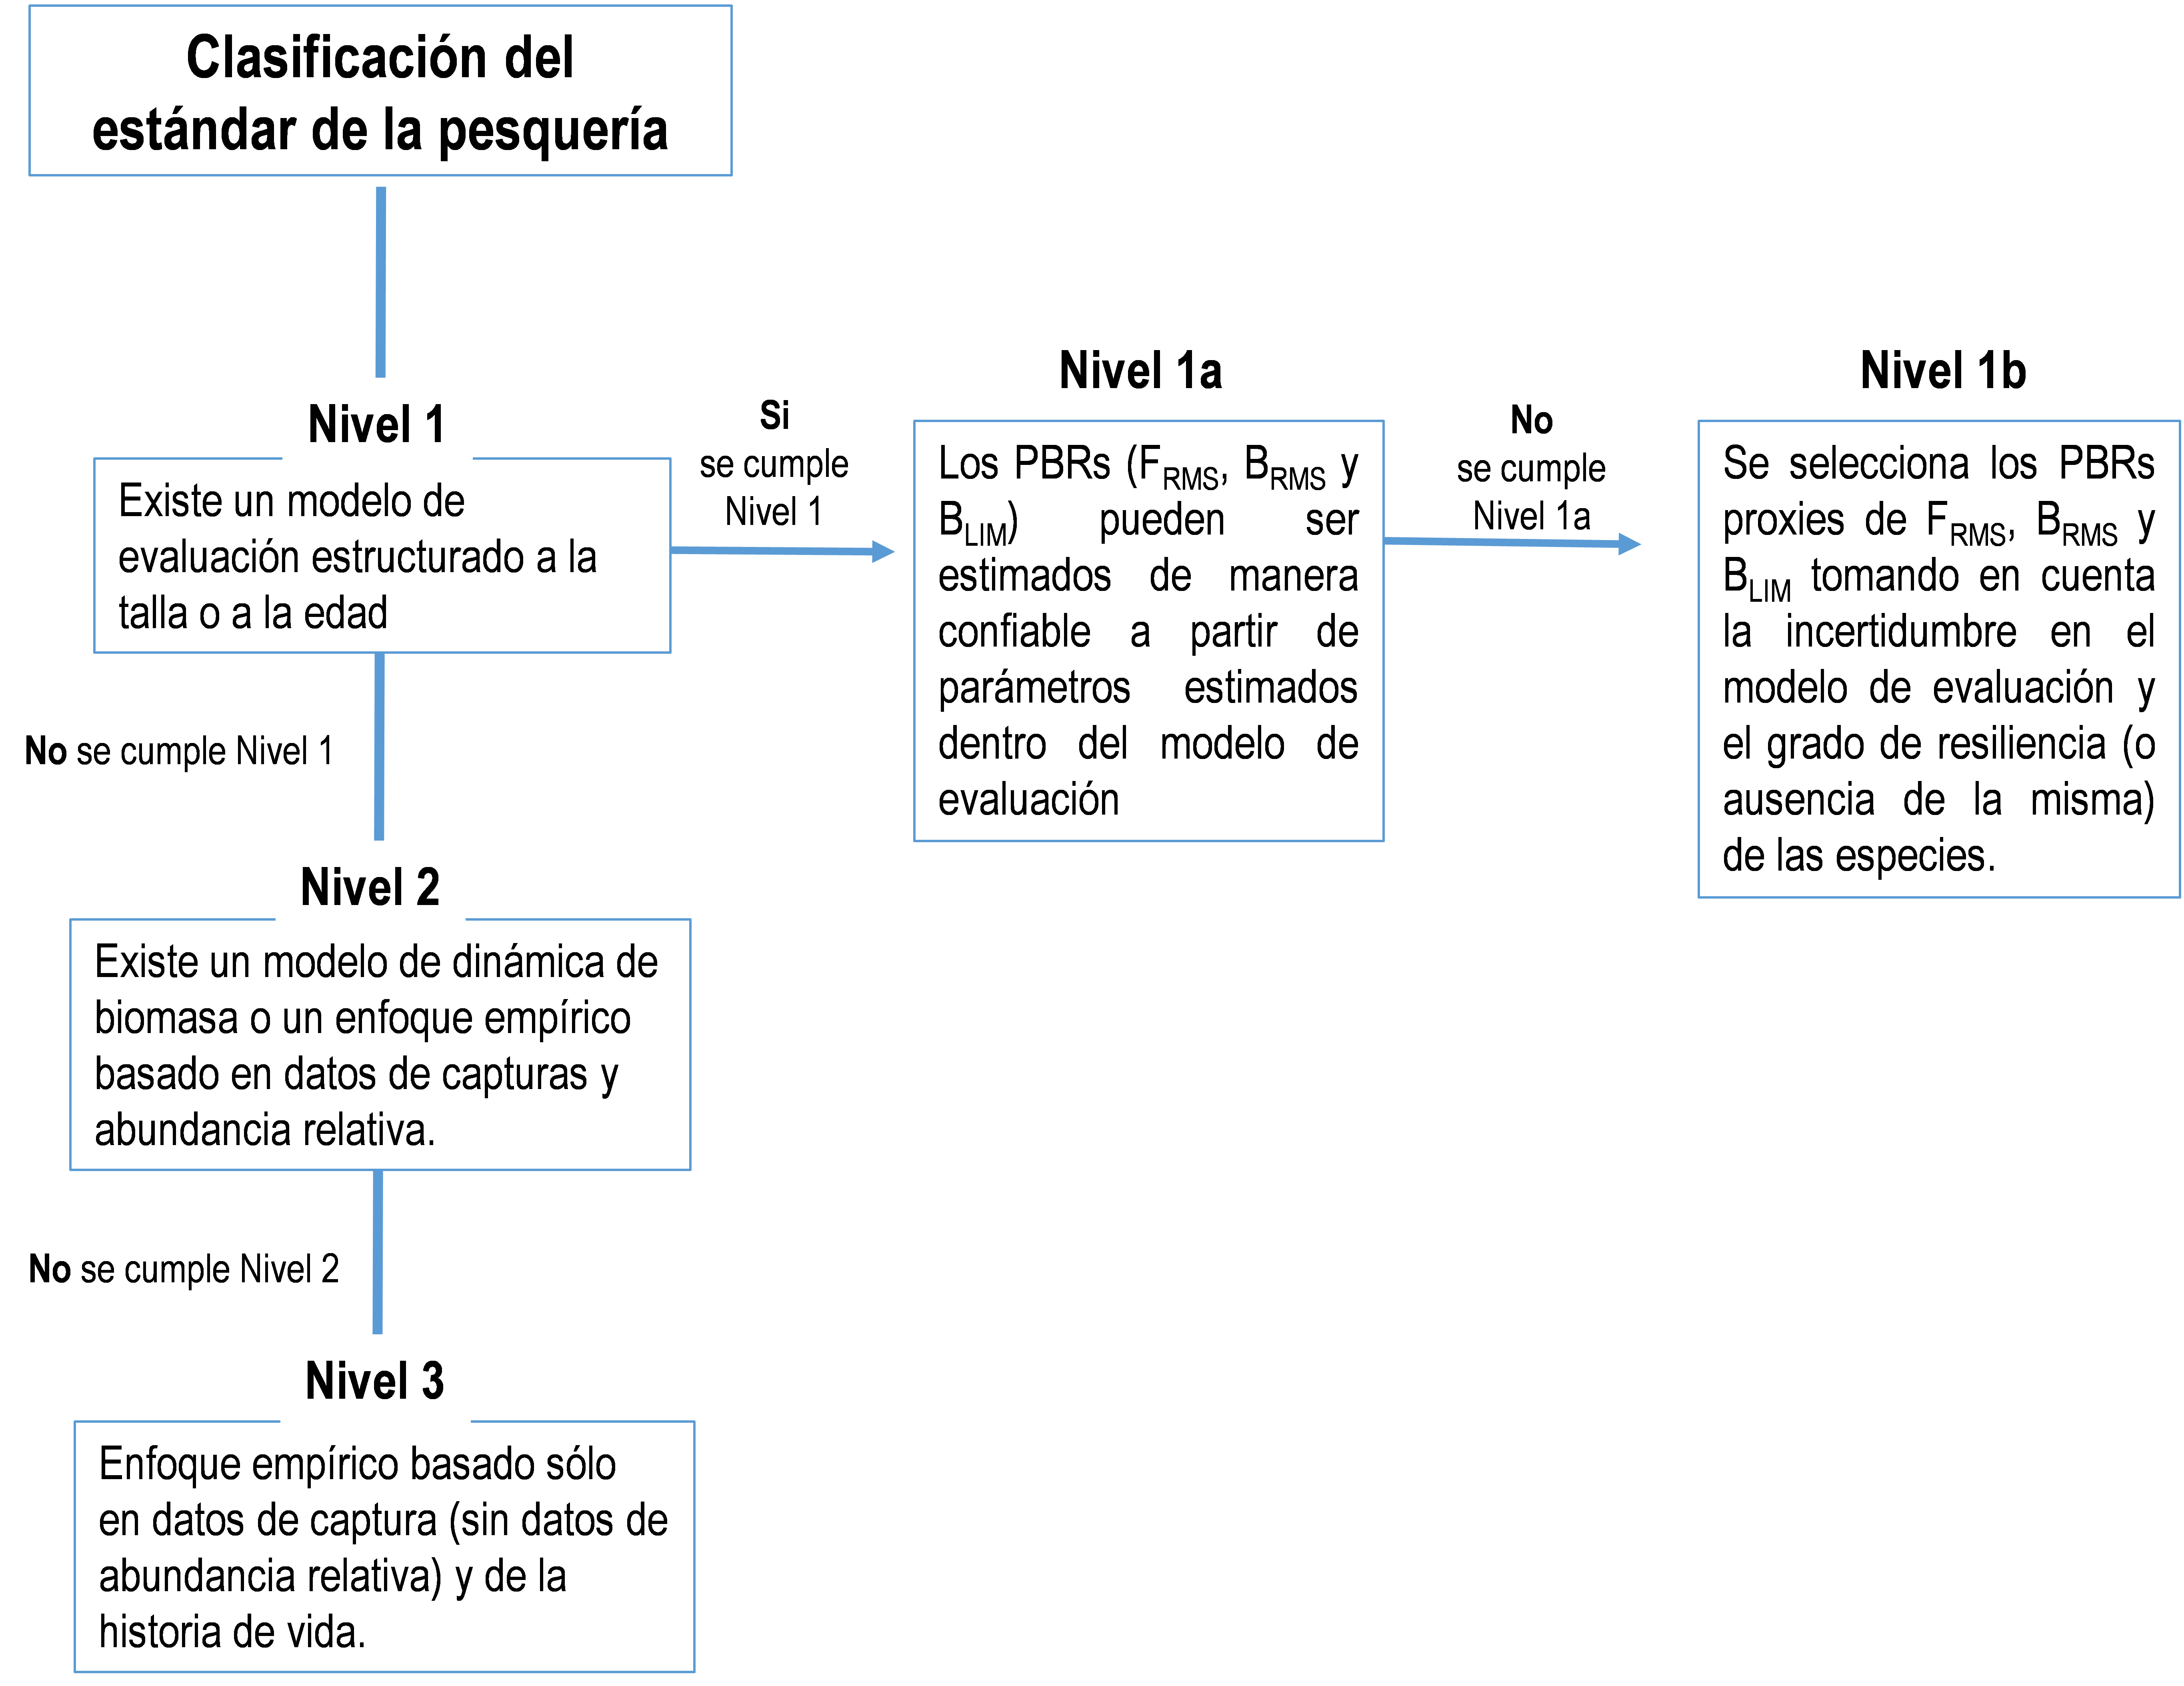
\includegraphics[width=0.8\textwidth]{Figuras/Figura_1.png}
\end{center}

\small \textbf{Figura 1}. Sistema de niveles para la determinación de
los PBRs de acuerdo a la cantidad, tipo y la calidad de la información
disponible y, métodos de evaluación de stock empleados en cada
pesquería. \vspace{0.5cm} \normalsize

Estimación de FRMS

Frente a la incertidumbre en la relación stock-recluta en merluza del
sur, la determinación de FRMS está basado en el análisis de biomasa
desovante por recluta que describen el cambio de la biomasa de una
cohorte o clase anual por efectos de la mortalidad natural y la pesca.
La biomasa adulta o desovante por recluta (bdpr) es obtenida como
función de la mortalidad por pesca (F), y en esta curva es factible
identificar el nivel de referencia biológico F\_(45\%bdpr) que se supone
debería minimizar el impacto de la pesca sobre el stock, permitiendo el
escape en torno al 45\% respecto del valor que existiría en ausencia de
explotación pesquera. La estimación de esta curva y su valor de
referencia (45\%bdpr) se obtiene por medio de la dinámica de la
abundancia en equilibrio definida como,

donde N\_a es la abundancia en número a la edad a+1 para una población
con longevidad máxima m, S\_(a-1) corresponde a la selectividad edad
específica, M es la mortalidad natural y F la mortalidad por pesca.

Basada en esta abundancia, la biomasa desovante por recluta se define
como,

donde dt es la fracción del año donde ocurre el desove (agosto), ma es
la fracción de peces maduros a la edad y es el peso medio a la edad. Con
el objeto de resolver el parámetro F\_RMS=F\_(45\%bdpr) se utilizó la
siguiente función objetivo

Diagrama de fases de explotación

El estado del recurso se estableció en base a la posición relativa de la
mortalidad por pesca y biomasa desovante versus los puntos biológicos de
referencia basado en el rendimiento máximo sostenible (RMS), tales como,
FRMS y BDRMS. De este modo se obtienen los indicadores del estatus
(F/FRMS y BD/BDRMS) que permiten construir un diagrama de fase, donde
los puntos de referencia biológicos se muestran en las líneas verticales
y horizontales en x=1 e y=1. Las líneas verticales indican la biomasa
desovante en el rendimiento máximo sostenible (BDRMS), bajo el cual el
recurso califica en sobreexplotación y biomasa desovante límite (BDLIM)
bajo el cual una pesquería califica de agotada y/o colapsada y la línea
horizontal el punto de referencia correspondiente a la mortalidad por
pesca en el rendimiento máximo sostenible (FRMS), sobre la cual el
recurso califica en sobreexplotación. La Figura 2 muestra el diagrama de
fase definido por el CCT-RDZSA para la pesquería de merluza del sur.

El estado de la pesquería en Plena Explotación se define en la Ley de
Pesca como ``un nivel en el que el punto biológico ha alcanzado o está a
su máximo rendimiento sostenido''. Debido a la variabilidad natural en
las condiciones ecológicas y ambientales, FRMS no es estática, pero
fluctuará alrededor de BDRMS. Para reconocer esta variabilidad, una
definición operativa para la región de Plena Explotación se define que
se extiende a ambos lados de los puntos de referencia de RMS. A
continuación, se describen los umbrales para la definición de estatus en
merluza del sur:

Sobrepesca: Este Comité consideró necesario diferenciar al interior de
la zona de sobreexplotación definida por la LGPA, el área de sobrepesca,
con el objeto de aplicar las medidas de Administración más acordes con
dicha condición. En tal sentido, la sobrepesca ocurriría cuando la
mortalidad por pesca F (variable de flujo y de control) exceda un valor
considerado umbral o límite, que en este caso corresponde al valor
superior en mortalidad por pesca (valor relativo al objetivo) de la zona
de plena explotación.

Sobreexplotado: En correspondencia con la definición anterior, la
sobreexplotación ocurriría cuando la biomasa (variable de estado) cae
bajo un valor umbral o límite, correspondiendo éste al valor inferior en
biomasa (valor relativo al objetivo) de la zona de plena explotación.

\begin{center}
\includegraphics[width=0.8\textwidth]{Figuras/Figura_2.png}
\end{center}

\small \textbf{Figura 2}. Diagrama de fase definido Comité Científico
Técnico de Recursos Demersales Zona Sur Austral (CCT-RDZSA) para la
pesquería de merluza del sur. \vspace{0.5cm} \normalsize

\hypertarget{objetivo-especuxedfico-3}{%
\subsection{3.3. Objetivo específico
3:}\label{objetivo-especuxedfico-3}}

\emph{``Analizar las distintas alternativas de Captura Biológicamente
Aceptable para estos stocks acorde con las estrategias de explotación y
reglas de control previamente definidas y considerando los posibles
estados de la naturaleza, con sus respectivos análisis de riesgo,
incluyendo análisis en horizontes de mediano y largo plazo, según
requerimiento.''}

Con objeto de actualizar las estimaciones de abundancia de merluza del
sur y definir un rango plausible de alternativas de Captura
Biológicamente Aceptable (CBA) para el año 2021, se realizarán las
siguientes tareas:

\begin{enumerate}
\def\labelenumi{\arabic{enumi}.}
\tightlist
\item
  Actualización de antecedentes y datos biológicos pesqueros hasta
  diciembre del año 2019 (Objetivo n°1)
\end{enumerate}

\begin{enumerate}
\def\labelenumi{\roman{enumi}.}
\tightlist
\item
  Solo las piezas de información derivadas directamente de la pesquería
  fueron actualizadas, esto es, las capturas por edad en las flotas
  participantes (arrastre, palangre y artesanal), los desembarques por
  flota corregidos por descarte y sub-reporte, los índices de abundancia
  basados en las tasas de captura de las flotas, los niveles de
  abundancia estimados durante los cruceros acústicos
\item
  Tanto los parámetros de historia de vida (pesos medios y madurez a la
  edad) y los ponderadores se mantuvieron iguales a los reportados en la
  asesoría anterior, esto con objeto de hacer comparable los resultados
\end{enumerate}

\begin{enumerate}
\def\labelenumi{\arabic{enumi}.}
\setcounter{enumi}{1}
\tightlist
\item
  Implementación del modelo de evaluación (Objetivo n°1)
\end{enumerate}

\begin{enumerate}
\def\labelenumi{\roman{enumi}.}
\tightlist
\item
  Implementación y codificación de los algoritmos de estimación en ADMB
\item
  Estimación de los parámetros (y errores estándar) poblacionales
  (e.g.~Ro, BDo) y variables de estado de importancia para el manejo de
  la pesquería (e.g.~biomasa desovante, reclutamientos)
\item
  Análisis de bondad de ajuste
\item
  Estimación de incertidumbre asociadas con las variables y parámetros
  claves
\end{enumerate}

\begin{enumerate}
\def\labelenumi{\arabic{enumi}.}
\setcounter{enumi}{2}
\tightlist
\item
  Actualización de PBR en base a los resultados de la evaluación de
  stock (Objetivo n°2)
\end{enumerate}

\begin{enumerate}
\def\labelenumi{\roman{enumi}.}
\tightlist
\item
  Biomasa Desovante y mortalidad por pesca respecto de las variables en
  el nivel del Rendimiento Máximo Sostenible
\item
  Biomasa Desovante límite a partir de la cual una pesquería califica de
  agotada o colapsada
\item
  PBR basados en el RMS
\end{enumerate}

\begin{enumerate}
\def\labelenumi{\arabic{enumi}.}
\setcounter{enumi}{3}
\tightlist
\item
  Exploración de los niveles de CBA para el año 2021 bajo diferentes
  ponderadores del FRMS.
\end{enumerate}

Cabe mencionar que estas tareas son transversalmente a todos los
objetivos específicos requeridos por el actual Convenio de Desempeño
2020-2021, el cual describe las directrices para los proyectos
orientados a la definición de `Estatus y posibilidades de explotación
biológicamente sustentables de los principales recursos pesqueros
nacionales año 2021'.

\hypertarget{protocolo-de-estimaciuxf3n-en-la-cba}{%
\subsection{3.3.1 Protocolo de estimación en la
CBA}\label{protocolo-de-estimaciuxf3n-en-la-cba}}

Como ha sido recurrente en la evaluación de la pesquería de merluza del
sur, existe un retardo en la disponibilidad de información biológica y
pesquera de al menos un año. Por lo que el protocolo de evaluación
consideraba los siguientes pasos para fijar la CBA al año siguiente
(2021):

\begin{enumerate}
\def\labelenumi{\arabic{enumi}.}
\tightlist
\item
  Actualizar la información biológica-pesquera hasta el año 2019 y
  estimar la abundancia a diciembre del año 2020.
\item
  Debido a que la evaluación de stock se realiza a lo largo del año 2020
  (temporada de pesca actual), la proyección de la abundancia
  poblacional desde diciembre del año 2019 a diciembre del año 2020, es
  realizada por descontar la máxima mortalidad que debe originar la CBA
  implementada durante el año 2020.
\item
  Finalmente, las alternativas de CBA para el año 2021 son calculadas
  por aplicar la mortalidad por pesca correspondiente al PBR objetivo (o
  sus ponderadores) sobre la abundancia estimada a diciembre del año
  2020.
\end{enumerate}

Sin embargo, siguiendo la solicitud realizada durante la última sesión
del el Comité Científico Técnico de Recursos Demersales Zona Sur Austral
(CCT-RDZSA), se realiza una proyección a tres años con el fin de estimar
una Captura Biológicamente Aceptable constante para el período
2021-2023.

\hypertarget{objetivo-especuxedfico-4}{%
\subsection{3.4. Objetivo específico
4:}\label{objetivo-especuxedfico-4}}

\emph{``Desarrollar los lineamientos técnicos e implementar la
aproximación de Evaluación de Estrategias de Manejo (EEM).''}

\hypertarget{evaluaciuxf3n-de-estrategias-de-manejo-eem}{%
\subsection{3.4.1 Evaluación de Estrategias de Manejo
(EEM)}\label{evaluaciuxf3n-de-estrategias-de-manejo-eem}}

Este objetivo muestra los avances en términos del desarrollo de los
procedimientos de manejo basado en simulación aplicados a la Merluza del
Sur bajo el marco del programa de Asesoría Integral para Pesca y
Acuicultura (ASIPA).

La evaluación de Estrategias de Manejo (EEM) tiene como principal meta
determinar cuál conjunto de Procedimientos de Manejo (PM) permite
alcanzar los objetivos de conservación o administración, bajo la premisa
que las gestiones de manejo fusionan aspectos políticos y técnicos. Un
procedimiento de manejo está conformado por tres elementos: i) los
puntos biológicos de referencia (PBR), ii) las reglas de control de
captura (RCC) y iii) los posibles escenarios de modelamiento basados en
un modelo de estimación de parámetros (MEP) de interés, en otras
palabras, un modelo de evaluación de stock. El proceso de comparación de
los diferentes PM en términos de medidas de desempeño (e.g.~P(objetivo)
es llamado una EEM.

Basado en los PBR, las RCC proporcionan las rutas temporales para
alcanzar los objetivos de manejo. En este sentido, bajo los criterios
establecidos por Ley de Pesca y Acuicultura respecto del RMS, los PBR
representan la componente técnica de un procedimiento de manejo pues
integran los aspectos de conservación que subyacen detrás de los PBR
basados en el RMS. Mientras que las RCC, deberían representar los
aspectos políticos ya que su forma y dimensión deberían incorporar los
requerimientos económicos, sociales y ambientales que regulan la
pesquería. En efecto, un conjunto de PBR sin RRC (adecuadas y bien
acordadas) no conforman un PM, y recae más bien en un ejercicio de
simulación bajo PBR que no necesariamente son reactivos en los periodos
futuros.

En este marco, se simulo la población de merluza del sur bajo
condiciones estocásticas en términos de su productividad, los PBR y
opciones de RCC, evaluando el desempeño de variables de estado en un
periodo de 50 años. Este acercamiento no está centrado en la capacidad
de estimación del MEP respecto de las variables poblacionales, sino, se
enfoca en la comparación de los diferentes PM bajo la precisa que la
información que alimenta el MEP en cada año de iteración proviene de
información perfecta deriva de un modelo operativo (MO) con iguales
características en términos del modelo de error (proceso y de
observación en variables de estado y en los datos generados) incluido en
el MEP.

Cabe señalar que los resultados de este objetivo son incipientes,
inapropiados para recomendaciones, y posiblemente variables en función
de la retroalimentación con la contraparte técnico de la SSPA y las
opiniones del CCT-RDZSA para la pesquería de merluza del sur.

\hypertarget{objetivo-especuxedfico-5}{%
\subsection{3.5. Objetivo específico
5:}\label{objetivo-especuxedfico-5}}

\emph{``Proponer el plan de trabajo para avanzar durante el año 2021 en
el cumplimiento del Programa de Mejoramiento Continuo de la Calidad de
la Asesoría Científica (PMCCAC), informando los logros esperados y su
vinculación con las siguientes etapas del Programa e informar del
cumplimiento de cada una de las recomendaciones realizadas en las
revisiones por pares, cuando corresponda y tareas complementarias
sugeridas por los CCT y/o evaluadores nacionales.''}

\hypertarget{programa-de-mejoramiento-contuxednuo-de-la-calidad-de-la-asesoruxeda-cientuxedfica-pmccac}{%
\subsection{3.5.1 Programa de Mejoramiento Contínuo de la Calidad de la
Asesoría Científica
(PMCCAC)}\label{programa-de-mejoramiento-contuxednuo-de-la-calidad-de-la-asesoruxeda-cientuxedfica-pmccac}}

En este objetivo se informan los avances alcanzados durante el
desarrollo de este estudio, conforme al Programa de Mejoramiento
Continuo de la Calidad de la Asesoría Científica (PMCCAC) elaborado por
recurso y/o pesquería. Este PMCCAC no sólo se enfoca en las brechas de
datos, información y conocimiento, sino que incluye la pertinencia,
consistencia, calidad y coherencia de éstos con la situación general de
la pesquería, acorde con los requerimientos de asesoría solicitados por
la administración pesquera.

No obstante, y con el propósito de alcanzar el Estándar Completo, se
identifican las brechas y limitaciones que impiden lograr ese objetivo y
se proponen detalladamente las acciones que se consideren necesarias
para alcanzarlo, en el corto o mediano plazo, según corresponda. Al
respecto, se reporta un listado de comprobación, en el que se da cuenta
técnica y detalladamente de todas las recomendaciones emanadas de los
revisores expertos, con el propósito de que, tanto los sectorialistas de
la Subsecretaría de Pesca, evaluadores externos, pares nacionales,
miembros del Comité Científico Técnico y cualquier científico, académico
y ciudadano puedan verificar el cumplimiento de cada una de las
observaciones, correcciones y recomendaciones señaladas por los
revisores.

Como parte integral de las actividades del proyecto, se considera la
participación en las reuniones establecidas por el CCT-RDZSA, así como
las actividades demandadas por la Revisión por Pares Externos e
Independientes (RPEI), las que constituirán el Estándar Metodológico en
la Evaluación, cuyos protocolos se mantendrán vigentes mientras una
actualización no sea requerida.

\pagebreak

\hypertarget{resultados}{%
\section{4. RESULTADOS}\label{resultados}}

\hypertarget{objetivo-especuxedfico-1-1}{%
\subsection{4.1. Objetivo específico
1:}\label{objetivo-especuxedfico-1-1}}

\emph{``Implementar procedimientos de evaluación de stock basados en
protocolos científicos para la determinación del estatus de merluza del
sur, con arreglo al nivel de información, conocimiento e incertidumbre
correspondiente, conforme a los estándares actuales en ciencia
pesquera.''}

\hypertarget{informaciuxf3n-bioluxf3gico-pesquera-1}{%
\subsection{4.1.1 Información
biológico-pesquera}\label{informaciuxf3n-bioluxf3gico-pesquera-1}}

\begin{enumerate}
\def\labelenumi{\alph{enumi})}
\tightlist
\item
  Desembarques y Descartes
\end{enumerate}

Los volúmenes de desembarques de merluza del sur se muestran en la Tabla
2 y Figura 3. Estos valores corresponden a la sumatoria de desembarques
oficiales en aguas de la unidad de pesquería norte y sur entre el
período 1977 y 2019 en el caso de la flota arrastrera industrial,
período 1987 y 2019 en el caso de la flota palangrera industrial, y
finalmente para la flota artesanal la sumatoria de los desembarques
informados entre las Regiones X-XII para el período 1981 y 2019.

Sin embargo, es conocido que las flotas tienen incentivos para el
descarte (principalmente la flota industrial) y subreporte (por parte de
la flota artesanal), conducidos principalmente por restricciones del
mercado y limitaciones en los niveles de cuotas de captura. Por ejemplo,
Quiroz (2016) mostró que los niveles de descarte por parte de las flotas
industriales son elevados, principalmente para la flota arrastrera donde
en promedio entre los años 2000 y 2019 el nivel de evasión alcanzo a un
valor promedio de 5665 toneladas, con un máximo de 7016 toneladas el año
2013. Menor participación en el descarte/subreporte se observó en la
flota artesanal, que en promedio alcanzó un nivel de evasión promedio
aproximado de 1219 toneladas para el periodo 2000-2019 (Figura 4).

Los valores de descarte-subreporte mencionados en el párrafo anterior
están basados en probables niveles históricos acordados en el seno del
Comité Científico Técnico de Recursos Demersales Zona Sur Austral
(CCT-RDZSA). Si bien estos niveles de descarte han posibilitado
reconstruir las series de desembarques oficiales (Tabla 3 y Figura 3),
el marco legal vigente indicado en el Artículo 7°B de la actual Ley
General de Pesca y Acuicultura (LGPA, N° 18.892) sostiene, que el
proceso de descarte en las pesquerías manejadas por cuotas de capturas
debe ser considerado en el establecimiento de la cuota global anual de
captura.

En este marco, la SSPA ha solicitado al IFOP que se considere el
descarte en la determinación del estatus y posibilidades de explotación
en las pesquerías nacionales, por medio de la incorporación de más
recientes recopilados en el marco del Programa de Investigación del
Descarte y Captura de Pesca Incidental (San Martín, 2016), o por medio
de proyectos licitados que hayan proporcionado esta información.

Tabla 2 Desembarques oficiales (toneladas) de las flotas de arrastre,
palangre y espinel artesanal.

Tabla 3 Desembarques corregidos (toneladas) de las flotas de arrastre,
palangre y espinel artesanal.

\begin{center}
\includegraphics[width=0.8\textwidth]{Figuras/Figura_3.png}
\end{center}

\small \textbf{Figura 3}. Línea punteada roja: desembarques oficiales
(miles de toneladas), línea punteada verde: desembarques corregidos de
merluza del sur (en base a Tabla 3 y 4), reportados por las flotas
industriales y flota artesanal para el periodo 1977-2019. \vspace{0.5cm}
\normalsize

\begin{center}
\includegraphics[width=0.8\textwidth]{Figuras/Figura_4.png}
\end{center}

\small \textbf{Figura 4}. Niveles de descarte/subreporte en toneladas
para las flotas industriales y artesanal durante el período 2000-2019.
\vspace{0.5cm} \normalsize

El Programa de Investigación del Descarte y Captura de Pesca Incidental,
entre otros objetivos, busca implementar y perfeccionar metodologías que
permitan evaluar espaciotemporalmente las capturas totales, retenidas y
descartadas de un número de especies incluida la merluza común (San
Martín et al., 2016). Mediante tres procedimientos alternativos de
estimación de la captura a bordo (cuya aplicación depende de la magnitud
de la captura) este programa recopila datos de la captura (retenida y
descartada) y su composición de tamaños mediante el despliegue de
observadores científicos especialmente entrenados para estos efectos.

Las estimaciones de la captura total (y sus fracciones retenida y
descartada y correspondientes varianzas) se obtienen mediante métodos
tanto diseño como modelo basados, y en el caso de merluza del sur, son
particularmente informativas tomando la información derivada de la flota
de arrastre. Por ejemplo, para el año. 2015 se estimó una captura de
10.198 t, con descartes de 4.104 t (40\% respecto del total). El factor
K se estimó en 1,6736 (Ver Tabla 4). En el año 2016, las capturas
totales se estimaron en 8.197 t, con porcentajes de descarte de 30\%.
Para este año se estimó un K de 1,4460 (Ver Tabla 5).

Tabla 4 Estimaciones de captura descartada, retenida y total de las
principales especies en la flota de arrastre hielero pesquería demersal
austral. Año 2015.

Tabla 5 Estimaciones de captura descartada, retenida y total de las
principales especies en la flota de arrastre hielero pesquería demersal
austral. Año 2016.

\begin{enumerate}
\def\labelenumi{\alph{enumi})}
\setcounter{enumi}{1}
\tightlist
\item
  Estructura de edades de las capturas comerciales
\end{enumerate}

Como es recurrente, la información de captura a la edad que es incluida
en el modelo de evaluación de stock de merluza del sur incluye registros
de tres flotas: (i) naves industriales arrastreras operando en aguas
exteriores, (ii) naves industriales palangreras con operaciones de pesca
principalmente en la zona extremo sur, y finalmente (iii) naves
artesanales que utilizan espineles de fondo desplegados principalmente
en aguas de la ZZE e interiores.

La información base de captura a la edad, proveniente del Sección
Edad-Crecimiento del Instituto de Fomento Pesquero, se encuentra
desagregada por sexo (macho-hembra), flota (las tres mencionadas
anteriormente) y área (norte y sur 47ºS). Para fines de la evaluación,
esta es agregada por flota por medio de la sumatoria de los individuos
muestreados por sexo, área y flota, ponderados por los niveles de
captura oficiales reportados por flota y área.

• Flotas industriales

Se actualizó la información completa del año 2019 totalizando un periodo
de datos de 37 años (1982-2019).

Como fue informado en previos reportes, la información edad estructurada
indica que entre los años 1981-1986 la flota arrastrera capturó
importantes niveles de peces longevos, que derivó en un declive
importante de la edad media de captura (Figura 5). Entre los años 1995 y
2005, las proporciones de peces longevos en ambas flotas fueron
reducidas en comparación con los años iniciales. No obstante, desde el
año 2012 la edad media se ha mantenido constante en torno a los 13-14
años en la flota arrastrera, mostrando una disminución hasta los 12 años
en 2019. A diferencia, la edad media de flota palangrera aumenta desde
el año 2012 hasta la actualidad, estancándose en los 15 años de edad.

Respecto del ingreso de cohortes a la población, la información
estructurada no posibilita un seguimiento adecuado, salvo las cohortes
nacidas en los años 1980 y 1986 que posiblemente sustentaron las
capturas durante la década de los años 90'.

\begin{center}
\includegraphics[width=0.8\textwidth]{Figuras/Figura_5.png}
\end{center}

\small \textbf{Figura 5}. Gráfico de burbujas de la proporción de las
edades en la captura de la flota arrastrera (superior) período 1989-2019
y palangrera (inferior) período 1981-2019. La línea verde representa la
edad media de la captura por año. \vspace{0.5cm} \normalsize

• Flota de espinel artesanal

Para el espinel la información disponible contempló los períodos
1987-1988, 1995-1997 Y 1999-2019 (Figura 6). La estructura de edades
abarca un rango edades más jóvenes que las flotas de arrastre y palangre
y una edad media de captura en torno a los 10 años (comparado a 12-14
años de las flotas industriales). Los dos primeros años de datos (1987 y
1988) corresponden a los años con grandes capturas artesanales (20 a 30
mil t), pero luego no se dispone de datos para el período 1989-1995,
donde las capturas aún eran altas, pero con tendencia a la baja. El
período 1995-1999, se aprecia el desplazamiento de la estructura hacia
edades mayores para luego observó una estructura relativamente estable
en los años 2005-2013. Por último, desde 2014 y hasta 2017 se observa un
incremento en la edad media desde los 9 hasta los 12 años, para decaer
nuevamente en 2018-2019 a los 11 años promedio.

\begin{center}
\includegraphics[width=0.8\textwidth]{Figuras/Figura_6.png}
\end{center}

\small \textbf{Figura 6}. Gráfico de burbujas de la proporción de las
edades en la captura de la flota artesanal período 1987-2019. La línea
verde representa la edad media de la captura por año. \vspace{0.5cm}
\normalsize

\begin{enumerate}
\def\labelenumi{\alph{enumi})}
\setcounter{enumi}{2}
\tightlist
\item
  Actualización de los cruceros hidroacústicos
\end{enumerate}

Biomasa disponible en la zona de desove

La información independiente de la pesquería utilizada en la evaluación
de merluza del sur corresponde a los cruceros acústicos desarrollados
durante el período de agregación reproductiva. Desde estos cruceros se
obtienen las claves talla-edad necesarias para generar matrices de
abundancia a la edad, las cuales son incluidas en el modelo de
evaluación para el período 2000-2019. Además, los cruceros reportan
estimaciones de biomasa desovante para el mismo período, que para su
inclusión en el modelo son considerados como valores de biomasa relativa
adulta.

Los cambios interanuales en la serie de biomasas acústicas sugieren una
reducción desde inicios de la serie para luego mantenerse relativamente
estables durante el período 2010-2015, la abundancia indica una
tendencia similar para el mismo periodo (Tabla 6 y Figura 7) con
aumentos considerables para los últimos dos años de prospección. La
biomasa y la abundancia tienen tendencias decrecientes muy similares,
excepto en los años 2008 y 2013, cuando los pesos promedios fueron
menores debido a la mayor presencia de peces de menores edades. Para los
años 2014 al 2019 la biomasa de merluza del sur presentó un aumento,
aunque este último año el peso medio fue menor que en años anteriores
(2587 g), se estimó una biomasa de 131433 toneladas. Tabla 6
Estimaciones del tamaño del stock (geoestadístico) en términos de
biomasa (t) y abundancia (millones), y pesos promedios estimados en los
cruceros hidroacústicos durante el período 2000-2019.

\begin{center}
\includegraphics[width=0.8\textwidth]{Figuras/Figura_7.png}
\end{center}

\small \textbf{Figura 7}. Biomasa miles de toneladas y abundancia
estimada en la zona de desove mediante acústica entre el período
2000-2019. \vspace{0.5cm} \normalsize

Estructura de edades del crucero

Con el fin de incluir solo la biomasa adulta del crucero acústico, desde
la asesoría año 2018, se utilizan las ojivas de madurez macroscópicas de
machos y hembras de cada año para el periodo 2000-2019 eliminando la
alta abundancia de ejemplares juveniles detectados durante los últimos 3
años. La distribución de la abundancia adulta por edades se ha mantenido
relativamente estable entre los 13 y 16 años Figura 8 (línea verde).

Para el año 2019 se registró una leve disminución de la edad media de la
fracción desovante, que alcanza los 15 años. Valores que no son posibles
de contrastar con el peso medio debido a la utilización de las ojivas de
madurez para separar ejemplares juveniles de adultos.

\begin{center}
\includegraphics[width=0.8\textwidth]{Figuras/Figura_8.png}
\end{center}

\small \textbf{Figura 8}. Gráfico de burbujas de la proporción de las
edades de la fracción desovante prospectada por los cruceros acústicos
período 2000-2019. La línea verde representa la edad media de la captura
por año. \vspace{0.5cm} \normalsize

\hypertarget{estandarizaciuxf3n-cpue-de-tasas-de-captura-flota-industrial}{%
\subsection{4.1.2 Estandarización CPUE de tasas de captura flota
industrial}\label{estandarizaciuxf3n-cpue-de-tasas-de-captura-flota-industrial}}

\begin{enumerate}
\def\labelenumi{\alph{enumi})}
\tightlist
\item
  Estandarización CPUE arrastre
\end{enumerate}

La base de datos proviene de las bitácoras de pesca de arrastre y
bitácoras de viajes pesca de IFOP, las que abarcan el período 1979-2019.
En la Tabla 7 se presenta el número de lances totales que se utilizaron
para el análisis. Desde inicios de la serie se presenta un valor en
torno a los 1000 registros anuales hasta el año 1998, donde los
registros aumentan a 6544. Posterior a esto, se observa un período en
torno a los 3500 registros (2004-2012), los años 2013-2015 presentan el
número de registros más bajo de toda la serie para aumentar en torno a
los 3 mil registros en los últimos años. El número total de registros
para el período es de 91439 lances. La estandarización se realiza
considerando dos períodos, el primero abarca desde 1979 hasta 1997 y el
segundo desde 1998 hasta 2018.

Tabla 7 Número de lances utilizados en la estandarización de CPUE por
año, período 1979-2019.

La Figura 9 contiene el histograma de los rendimientos de pesca (CPUE) y
el logaritmo de la CPUE incluyendo los 18208 lances para el período 1
(1979-1997) y 73231 lances para el período 2 (1998-2019). El valor en
logaritmo presenta la condición de normalidad necesaria para la
estandarización del rendimiento. Esta variable se mide en kilógramos por
horas de arrastre (kg/h.a.).

\begin{center}
\includegraphics[width=0.8\textwidth]{Figuras/Figura_9.png}
\end{center}

\small \textbf{Figura 9}. Histograma del rendimiento de pesca en
kilógramos por hora de arrastre y del logaritmo del rendimiento para el
período 1 (1979-1997) y período 2 (1998-2019). \vspace{0.5cm}
\normalsize

La Figura 10 presenta los valores promedio para las horas de arrastre,
CPUE y captura durante el período 2 (1998-2019). En las horas de
arrastre se observa una importante disminución para el año 2002 en donde
el valor decae hasta las 1.99 horas de arrastre, gracias al bajo aporte
del buque 400180 en ese año en particular. Existe un aumento progresivo
en la hora de arrastre promedio desde el año 2002 hasta la actualidad,
en donde el año 2019 alcanza el valor más alto de la serie (4.0 h.a.).
En cuanto a las capturas y CPUE promedio se observa el mismo aumento
desde inicios de la serie. El año 2014 presenta valores bajos tanto en
captura y CPUE debido a la importante disminución de las cuotas de
captura.

\begin{center}
\includegraphics[width=0.8\textwidth]{Figuras/Figura_10.png}
\end{center}

\small \textbf{Figura 10}. Valores promedio de horas de arrastre,
captura (kg) y CPUE nominal (kg/h.a.) por año para el período 2
(1998-2019) flota arrastrera. \vspace{0.5cm} \normalsize

Para incorporar la intencionalidad de pesca como un predictor en los
modelos lineales de predicción de las tasas de captura, se construyeron
las matrices con composición de captura para cada lance. Una vez
obtenida la matriz de proporción de especies por cada lance, se realizó
un análisis de componentes principales con el fin de reducir el número
de especies y obtener solo aquellas que explican más de un 85\% de la
varianza. Con estas nuevas especies se realizó el análisis de cluster a
través del método de K-means y como medida de similitud se usó la
distancia euclidiana, reduciendo el número total de registros a 1500
centroides. Por ejemplo, en la Figura 11 se presentan los primeros 5
componentes principales para el período 2 obtenidos en la etapa
anterior, el primero contiene presencia de merluza de cola y merluza del
sur relacionada positivamente, el segundo contiene las mismas especies,
pero relacionadas de forma negativa, el tercero se caracteriza por
congrio y los dos últimos por merluza de tres aletas y bycatch.

\begin{center}
\includegraphics[width=0.8\textwidth]{Figuras/Figura_11.png}
\end{center}

\small \textbf{Figura 11}. Análisis de componentes principales de la
matriz de proporciones para el arrastre, período 2 (1998-2019).
\vspace{0.5cm} \normalsize

Finalmente, se construyó el dendrograma y se recuperaron los datos
originales (lances de pesca) reducidos en las etapas anteriores para
asignarlos a un cluster o táctica de pesca determinado, obteniendo un
set de datos con el número de cluster y la proporción de especies
correspondiente, el número de registros utilizados finalmente en cada
cluster se presenta en la Tabla 8. La estandarización de la CPUE utiliza
la táctica de pesca como variables categóricas en el modelo lineal
generalizado. Tabla 8 Número de lances incorporados en cada cluster para
el período 1 (1979-1997) y período 2 (1998-2019).

Este arte de pesca se caracteriza por presentar un gran número de
especies, pero la mayoría con bajos porcentajes en cuanto a
representatividad según la Figura 12 y 13. En el período 1 la especie
predominante en el cluster uno corresponde a merluza del sur, el cluster
dos presenta un mix de especies, el tres se caracteriza por presentar
aproximadamente un 50\% de merluza del sur y por último el cluster
cuatro y cinco con una mayor proporción de merluza de cola y congrio
respectivamente (Figura 12).

\begin{center}
\includegraphics[width=0.8\textwidth]{Figuras/Figura_12.png}
\end{center}

\small \textbf{Figura 12}. Proporción de especies presentes en los
lances por cada cluster para el período 1 (1979-1997). \vspace{0.5cm}
\normalsize

El análisis para el segundo período (1998-2019) se presenta en la Figura
13, se observa que en el cluster uno existe un mix de especies con menor
importancia en proporción, el cluster dos se caracteriza principalmente
por merluza del sur, el número tres contiene principalmente bycatch y,
por último, el cluster cuarto una proporción importante de merluza de
cola.

\begin{center}
\includegraphics[width=0.8\textwidth]{Figuras/Figura_13.png}
\end{center}

\small \textbf{Figura 13}. Proporción de especies presentes en los
lances por cada cluster para el período 2 (1998-2019). \vspace{0.5cm}
\normalsize

Las Figuras 14 y 15 confirman los resultados anteriormente descritos, la
Figura 14 presenta la intencionalidad de pesca para el período 1 en el
cluster 1, en donde la proporción de merluza del sur por lance es alta.
La Figura 15, confirma los resultados obtenidos en el período 2
identificándose el cluster dos con los mayores valores de captura y
CPUE, cluster que corresponde al con mayor proporción de merluza del
sur. En esta figura se observa un aumento progresivo en la CPUE promedio
anual del cluster dos, la cual disminuye durante los últimos cinco años
de la serie.

\begin{center}
\includegraphics[width=0.8\textwidth]{Figuras/Figura_14.png}
\end{center}

\small \textbf{Figura 14}. Frecuencia de la proporción de merluza del
sur en la flota arrastrera para el período 1, por año en el cluster 1.
\vspace{0.5cm} \normalsize

\begin{center}
\includegraphics[width=0.8\textwidth]{Figuras/Figura_15.png}
\end{center}

\small \textbf{Figura 15}. Sumatoria anual de la captura kg y esfuerzo
en h.a., CPUE nominal promedio kg/h.a. para la flota arrastrera para el
período 2 por cluster, el tamaño del circulo es proporcional al número
de lances utilizados. \vspace{0.5cm} \normalsize

Para la estandarización de la CPUE en el período 1 se implementaron
cinco modelos, incorporando como factores el año, mes, buque, zona y
cluster. En la Tabla 9 se presentan los estadísticos para cada modelo,
siendo en primer lugar el factor año el que explica un mayor porcentaje
de la devianza (26-33\%), seguido por el factor mes y cluster y por
último el factor zona. El modelo que explica un mayor porcentaje de la
devianza total corresponde a mod1 (67\%).

Tabla 9 Estadísticos de los modelos lineales con su respectiva devianza
explicada en porcentaje, período 1 (1979-1997).

Para el período 2 se implementaron 4 modelos, incorporando como factores
el año, mes, zona y cluster. En la Tabla 10 se presentan los
estadísticos para cada modelo, siendo en primer lugar el factor cluster
el que explica un mayor porcentaje de la devianza para todos los casos
(entre un 13 y 18\%), seguido por el factor mes (8 -- 8.7\%) y por
último el factor zona. El modelo que explica un mayor porcentaje de la
devianza total corresponde a mod0 (39.7\%) seguido de mod3 (35.2\%).

Tabla 10 Estadísticos de los modelos lineales con su respectiva devianza
explicada en porcentaje, período 2 (1998-2019).

En la Figura 16 se presenta la CPUE estandarizada para la flota
arrastrera período 1 para los 5 modelos probados Mod0, Mod1, Mod2, Mod3,
Mod4 y la CPUE promedio sin estandarizar en línea celeste. Las CPUE´s
escaladas de cada modelo presentan la misma tendencia que la CPUE
promedio anual evidenciando una progresiva disminución desde inicios del
periodo hasta el año 1995 donde se comienza a observar un leve aumento.

\begin{center}
\includegraphics[width=0.8\textwidth]{Figuras/Figura_16.png}
\end{center}

\small \textbf{Figura 16}. CPUE (kg/h.a.) media y estandarizada para la
flota arrastrera período 1979-1997. Se presentan los 5 modelos probados
y la CPUE promedio sin estandarizar en línea celeste. \vspace{0.5cm}
\normalsize

Para el período 2, la CPUE estandarizada se presenta en la Figura 17. En
líneas segmentadas se presenta la CPUE estimada por los 4 modelos de
estandarización Mod0, Mod1, Mod2, Mod3, en línea continua roja la CPUE
promedio sin estandarizar y en línea continua amarilla la CPUE
estandarizada estimada el año anterior (informe de estatus 2018). En
este período se observa un aumento en la CPUE que proviene de fines del
período 1.

\begin{center}
\includegraphics[width=0.8\textwidth]{Figuras/Figura_17.png}
\end{center}

\small \textbf{Figura 17}. CPUE kg/h.a. estandarizada para la flota
arrastrera período 2 (1998-2019). Se presentan los 4 modelos probados en
líneas segmentadas, CPUE promedio sin estandarizar en línea continua
roja y CPUE estandarizada (informe estatus año 2018) en línea continua
amarilla. \vspace{0.5cm} \normalsize

\begin{enumerate}
\def\labelenumi{\alph{enumi})}
\setcounter{enumi}{1}
\tightlist
\item
  Estandarización CPUE palangre
\end{enumerate}

La captura por unidad de esfuerzo (CPUE) en el palangre fue medida en
kilógramos por número de anzuelo por hora de reposo (kg/(nanz*h.r.)). La
base de datos utilizada comprende dos períodos 1987- 1997 y 1998-2018.
En las Tablas 11 y 12 se presenta el número de registros por año y por
pesquería, posterior a los filtros realizados a la base de datos. El
período 1 cuenta con 20722 registros mientras que el período 2 con
15738. Las pesquerías dirigidas a merluza del sur corresponden a la
número 5 (IFOP) y número 92 (SERNAP) y las pesquerías número 11 y 91
corresponden a palangre fábrica bacalao IFOP y SERNAP respectivamente.

Tabla 11 Número de registros de la flota palangrera para el período 1
(1987-1997) por año y por pesquería 5= flota merlucera (IFOP), 10=
palangre hielero (IFOP) y 11=palangre fábrica (IFOP).

Tabla 12 Número de registros para la flota palangrera para el período 2
(1998-2019) por año y por pesquería, 5=Palangre fábrica merlucero
(IFOP), 11= Palangre fábrica bacalao (IFOP), 91= Palangre fábrica
bacalao (SERNAP) y 92= Palangre fábrica merlucero (SERNAP).

La Figura 18 contiene el histograma de los rendimientos de pesca (CPUE)
y el logaritmo de la CPUE para ambos períodos. El valor en logaritmo
presenta la condición de normalidad necesaria para la estandarización
del rendimiento. Esta variable se mide en kilógramos por número de
anzuelo por hora de reposo (kg/(nanz*h.r.)).

\begin{center}
\includegraphics[width=0.8\textwidth]{Figuras/Figura_18.png}
\end{center}

\small \textbf{Figura 18}. Histograma del rendimiento y logaritmo del
rendimiento de pesca en kilógramos por número de anzuelo y hora de
reposo. \vspace{0.5cm} \normalsize 

La Figura 19 entrega un resumen de los datos de palangre utilizados en
el período 2 (1998-2019), el cuadrante superior izquierdo contiene el
número de anzuelos promedio para cada pesquería, el valor bordea los 15
mil anzuelos exceptuando algunos años (por ejemplo 2015). En la
pesquería 11 el valor más bajo se encuentra en el año 2013 ya que el
barco 941225 presenta solo 3600 anzuelos ese año, a diferencia del resto
de los barcos que presentan entre 11 mil y 24 mil anzuelos.

En el cuadrante superior derecho se presenta la CPUE promedio con las
horas de reposo no corregidas, en el cuadrante inferior izquierdo la
captura promedio de merluza del sur, en donde los años 2017, 2018 y 2019
se caracterizaron por presentar los valores más bajos de la serie, y en
el cuadrante inferior derecho la CPUE promedio considerando las horas de
reposo corregidas.

\begin{center}
\includegraphics[width=0.8\textwidth]{Figuras/Figura_19.png}
\end{center}

\small \textbf{Figura 19}. Valores promedio del número de anzuelos por
año y pesquería (5,11,91,92) (cuadrante superior izquierdo), captura
promedio de merluza del sur por año en kilogramos (cuadrante inferior
izquierdo), CPUE nominal promedio por año con horas de reposo sin
corregir (cuadrantes superior derecho) y CPUE nominal promedio por año
con horas de reposo corregidas (cuadrantes inferior derecho) para el
período 2 (1998-2019) flota palangrera. \vspace{0.5cm} \normalsize 

Al igual que en el arrastre, se construyeron matrices con composición de
captura para cada lance con el fin de incorporar la intencionalidad de
pesca como un predictor en los modelos lineales. Luego, se realizó el
análisis de componentes principales y el análisis de cluster obteniendo
como resultado la Figura 20, aquí se presentan los primeros 5
componentes principales del período 2 obtenidos en la etapa anterior, el
primero contiene presencia de merluza del sur y congrio relacionada
positivamente, el segundo contiene las mismas especies, pero
relacionadas de forma negativa, el tercero se caracteriza por brótula y
el cuarto por bycatch y el último por merluza de cola.

\begin{center}
\includegraphics[width=0.8\textwidth]{Figuras/Figura_20.png}
\end{center}

\small \textbf{Figura 20}. Análisis de componentes principales de la
matriz de proporciones para el palangre, periodo 2 (1998-2019).
\vspace{0.5cm} \normalsize 

Luego se construyó el dendrograma y se recuperaron los datos originales
(lances de pesca) reducidos en las etapas anteriores para asignarlos a
un cluster o táctica de pesca determinado, obteniendo un set de datos
con el número de cluster y la proporción de especies correspondiente, el
número de registros utilizados finalmente en cada cluster se presenta en
la Tabla 13.

Tabla 13 Número de lances incorporados en cada cluster.

Contrario a lo obtenido en la flota arrastrera, donde pocos cluster
contienen proporciones elevadas de captura de merluza del sur, aquí se
observan cluster con mix de especies, la flota palangrera concentra las
mayores proporciones de captura en más de un cluster, por ejemplo, la
Figura 21 contiene la proporción de especies por cluster para el período
1, en donde se observa presencia importante de merluza del sur en los
cluster 1 y 2 dejando en el cluster 3 mayor participación de congrio.
Para el período dos (Figura 22) se observan 4 cluster en donde existe
una importante presencia de merluza en los cluster 1, 3 y 4.

\begin{center}
\includegraphics[width=0.8\textwidth]{Figuras/Figura_21.png}
\end{center}

\small \textbf{Figura 21}. Proporción de especies presentes en los
lances de la flota palangrera por cada cluster, período 1 (1979-1997).
\vspace{0.5cm} \normalsize    

\begin{center}
\includegraphics[width=0.8\textwidth]{Figuras/Figura_22.png}
\end{center}

\small \textbf{Figura 22}. Proporción de especies presentes en los
lances de la flota palangrera por cada cluster, período 2 (1997-2019).
\vspace{0.5cm} \normalsize    

La Figura 23 contiene la intencionalidad de pesca del cluster 2 para el
período 1, este cluster es el que contiene la mayor proporción de
merluza del sur en las capturas (según Figura 21), esta figura confirma
los resultados anteriores identificando proporciones altas de merluza
del sur por cada lance.

\begin{center}
\includegraphics[width=0.8\textwidth]{Figuras/Figura_23.png}
\end{center}

\small \textbf{Figura 23}. Frecuencia de la proporción de merluza del
sur para la flota palangrera período 1 (1979-1997) por año en el cluster
2. \vspace{0.5cm} \normalsize    

El cluster con mayor proporción de merluza del sur para el período 2
corresponde al cluster 3, seguido del cluster 1 (según Figura 22), la
Figura 24 presenta la captura, esfuerzo y CPUE promedio por cada
cluster. La línea celeste corresponde al cluster 3, alcanzando los
valores más altos de captura y CPUE promedio.

\begin{center}
\includegraphics[width=0.8\textwidth]{Figuras/Figura_24.png}
\end{center}

\small \textbf{Figura 24}. Sumatoria anual de la captura (kg) y esfuerzo
(nanz/h.r.), CPUE (kg/(nanz*h.r.)) por cluster para el período 2 período
1998-2019, el tamaño del circulo es proporcional al número de lances
utilizados. \vspace{0.5cm} \normalsize   

Para la estandarización de la CPUE se utilizaron 4 modelos lineales
generalizados, los que incluyeron como factores el año (1998-2019), mes,
pesquería, zona, cluster y barco. En la Tabla 14 y 15 se presentan los
estadísticos para cada MLG.

El análisis de varianza de los predictores para el período 1 (1979-1997)
indica que la táctica de pesca y año son los factores que mejor explican
la varianza de la CPUE (hasta un 19\%). El modelo que explica un mayor
porcentaje de la varianza corresponde al modelo 1 con un 44\%.

El período dos (1998-2019) presenta resultados similares en donde el
predictor cluster alcanza un 35.3\% de la devianza explicada. Esto
sugiere que el predictor ``táctica de pesca'' es adecuado para construir
una serie de CPUE objetiva en una pesquería multi específica, filtrando
adecuadamente la intencionalidad de pesca. En segundo lugar, encontramos
el factor mes que explica entre un 9.2 y 15.7\%. El modelo que explica
un mayor porcentaje de la devianza total corresponde al modelo 1
(61.1\%) seguido del mod2 (51\%).

Tabla 14 Estadísticos de los modelos lineales para el período 1
(1979-1997) con su respectiva devianza explicada en porcentaje.

Tabla 15 Estadísticos de los modelos lineales para el período 2
(1998-2019) con su respectiva devianza explicada en porcentaje.

La CPUE estandarizada para la flota palangrera se presenta en la Figura
25 y 26. El período 1 considera los 4 modelos utilizados Mod0, Mod1,
Mod2, Mod3, en línea continua celeste se muestra la CPUE promedio sin
estandarizar. Para el período 2, la Figura 26 incluye la CPUE de los
modelos utilizados en líneas segmentadas, la CPUE promedio sin
estandarizar en línea continua roja y la CPUE estandarizada estimada el
año anterior en línea continua amarilla (informe de estatus 2018).

\begin{center}
\includegraphics[width=0.8\textwidth]{Figuras/Figura_25.png}
\end{center}

\small \textbf{Figura 25}. CPUE estandarizada (kg/(nanz*h.r.)) período
1, para los 4 modelos probados en líneas segmentadas, CPUE promedio sin
estandarizar en línea continua roja y CPUE estandarizada (informe
estatus año 2018) en línea continua amarilla. \vspace{0.5cm} \normalsize

\begin{center}
\includegraphics[width=0.8\textwidth]{Figuras/Figura_26.png}
\end{center}

\small \textbf{Figura 26}. CPUE estandarizada (kg/(nanz*h.r.)) período
2, para los 4 modelos probados en líneas segmentadas, CPUE promedio sin
estandarizar en línea continua roja y CPUE estandarizada (informe
estatus año 2018) en línea continua amarilla. \vspace{0.5cm} \normalsize

\hypertarget{ajustes-modelo-base}{%
\subsection{4.1.3 Ajustes modelo base}\label{ajustes-modelo-base}}

El modelo base actual (Mod0\_03a) proviene del escenario Mod0\_03
implementado en la asesoría año 2019. Este modelo se caracteriza por
estandarización de la CPUE de arrastre y palangre en dos períodos.
Además, incluye el índice de abundancia de la flota artesanal en la
función de verosimilitud y la táctica de pesca como un predictor en los
modelos lineales de predicción de tasas de captura. Además, se
incorporan algunas modificaciones solicitadas por la Subsecretaría de
Pesca y Acuicultura y por el Comité Científico Técnico de Recursos
Demersales: i) modificación del coeficiente de capturabilidad para el
arrastre considerando años de quiebre 1997, 2001 y 2011 y para el
palangre los años 1997 y 2011; ii) modificación del coeficiente de
variación para los índices de abundancia: los pesos para los índices de
las flotas arrastrera y palangrera se redujeron a la mitad mientras que
el crucero acústico se aumentó al doble. El índice de CPUE de la flota
artesanal no se modificó, manteniendo un peso de baja importancia
respecto de los restantes índices de abundancia; iii) incorporación de
la fracción madura del crucero acústico, en donde se utilizaron las
ojivas de madurez macroscópicas de machos y hembras de cada año para el
periodo 2000-2019; iv) incorporación de pesos medios variables entre
años para las flotas y el crucero acústico.

Como datos de entrada provenientes de la pesquería se cuenta con:

• (*) Captura a la edad:

39 años de datos para el arrastre (1981-2019). 29 años para palangre
(1989-1992, 1995-2019). 26 años para espinel artesanal (1987, 1988,
1995-1997, 1999- 2019). 19 años de datos de abundancia provenientes del
crucero (2000-2005, 2007-2019).

• Índices de abundancia:

Arrastre (1979-2019). Palangre (1987-2019). Artesanal (2000-2019).
Crucero (2000-2019).

• Desembarques:

Arrastre (1977-2019). Palangre (1987-2019). Artesanal (1981-2019).

La Tabla 16 contiene los valores del coeficiente de variación utilizado
para los índices de abundancia provenientes de las flotas de arrastre,
palangre, artesanal y crucero acústico.

Tabla 16 Coeficientes de variación para el índice de abundancia CPUE
utilizados para las flotas de arrastre, palangre, artesanal y crucero
acústico Modelo0\_03a.

La Figura 27 presenta el ajuste de los desembarques de las flotas
arrastrera, palangrera y artesanal con sus respectivos residuales por
flota (Figura 28). Se observa que los ajustes de las series temporales
son precisos e inclusive reproducen la reducción de los desembarques
posterior al año 2010. Los desembarques de las flotas palangreras y
artesanal disminuyen durante los últimos 4 años, a diferencia de la
flota de arrastre que presenta un aumento en los últimos 3 años debido
al traspaso de cuota de la flota artesanal.

\begin{center}
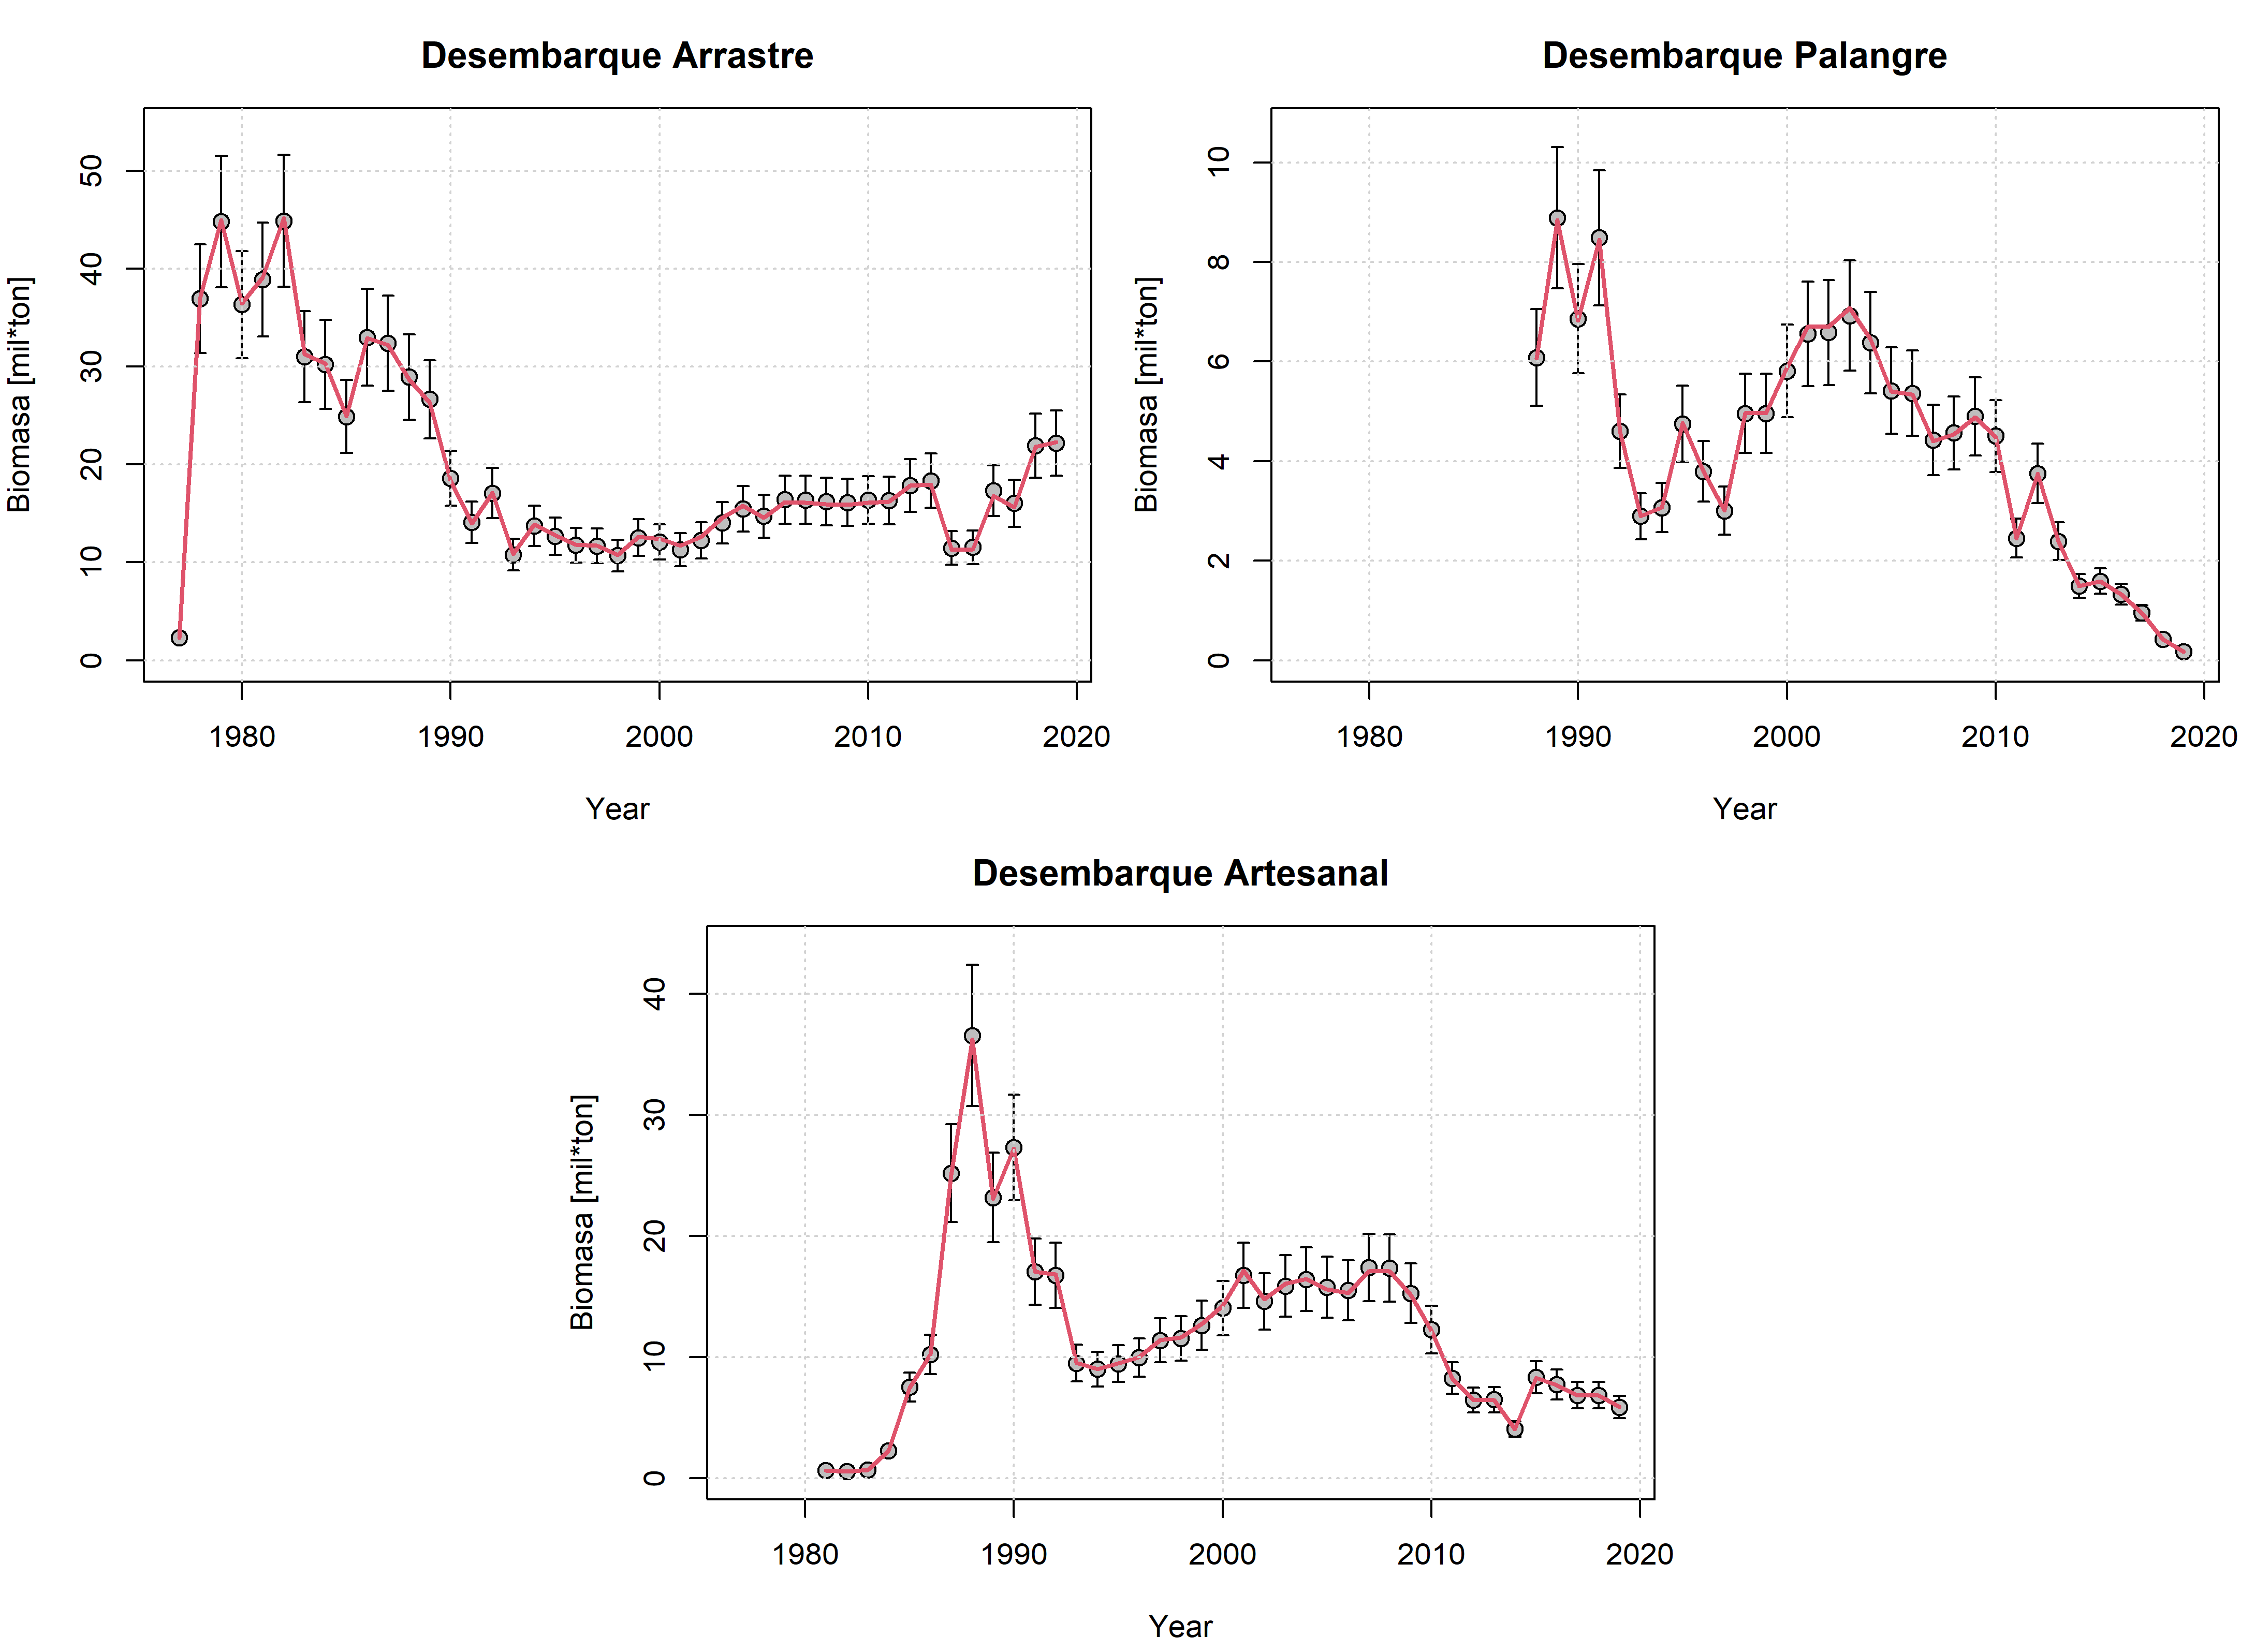
\includegraphics[width=0.8\textwidth]{Figuras/FitY.png}
\end{center}

\small \textbf{Figura 27}. Desembarque observado en miles de toneladas
(puntos) y estimado (línea roja) con su respectiva desviación estándar
(barras) para las flotas arrastrera, palangrera y artesanal.
\vspace{0.5cm} \normalsize

La precisión del ajuste se muestra en el comportamiento de los
residuales, los que se sobreponen con la distribución teórica esperada
para la distribución normal de datos (Figura 28). Solo unos pocos puntos
de datos se alejan de dos desviaciones estándar.

\begin{center}
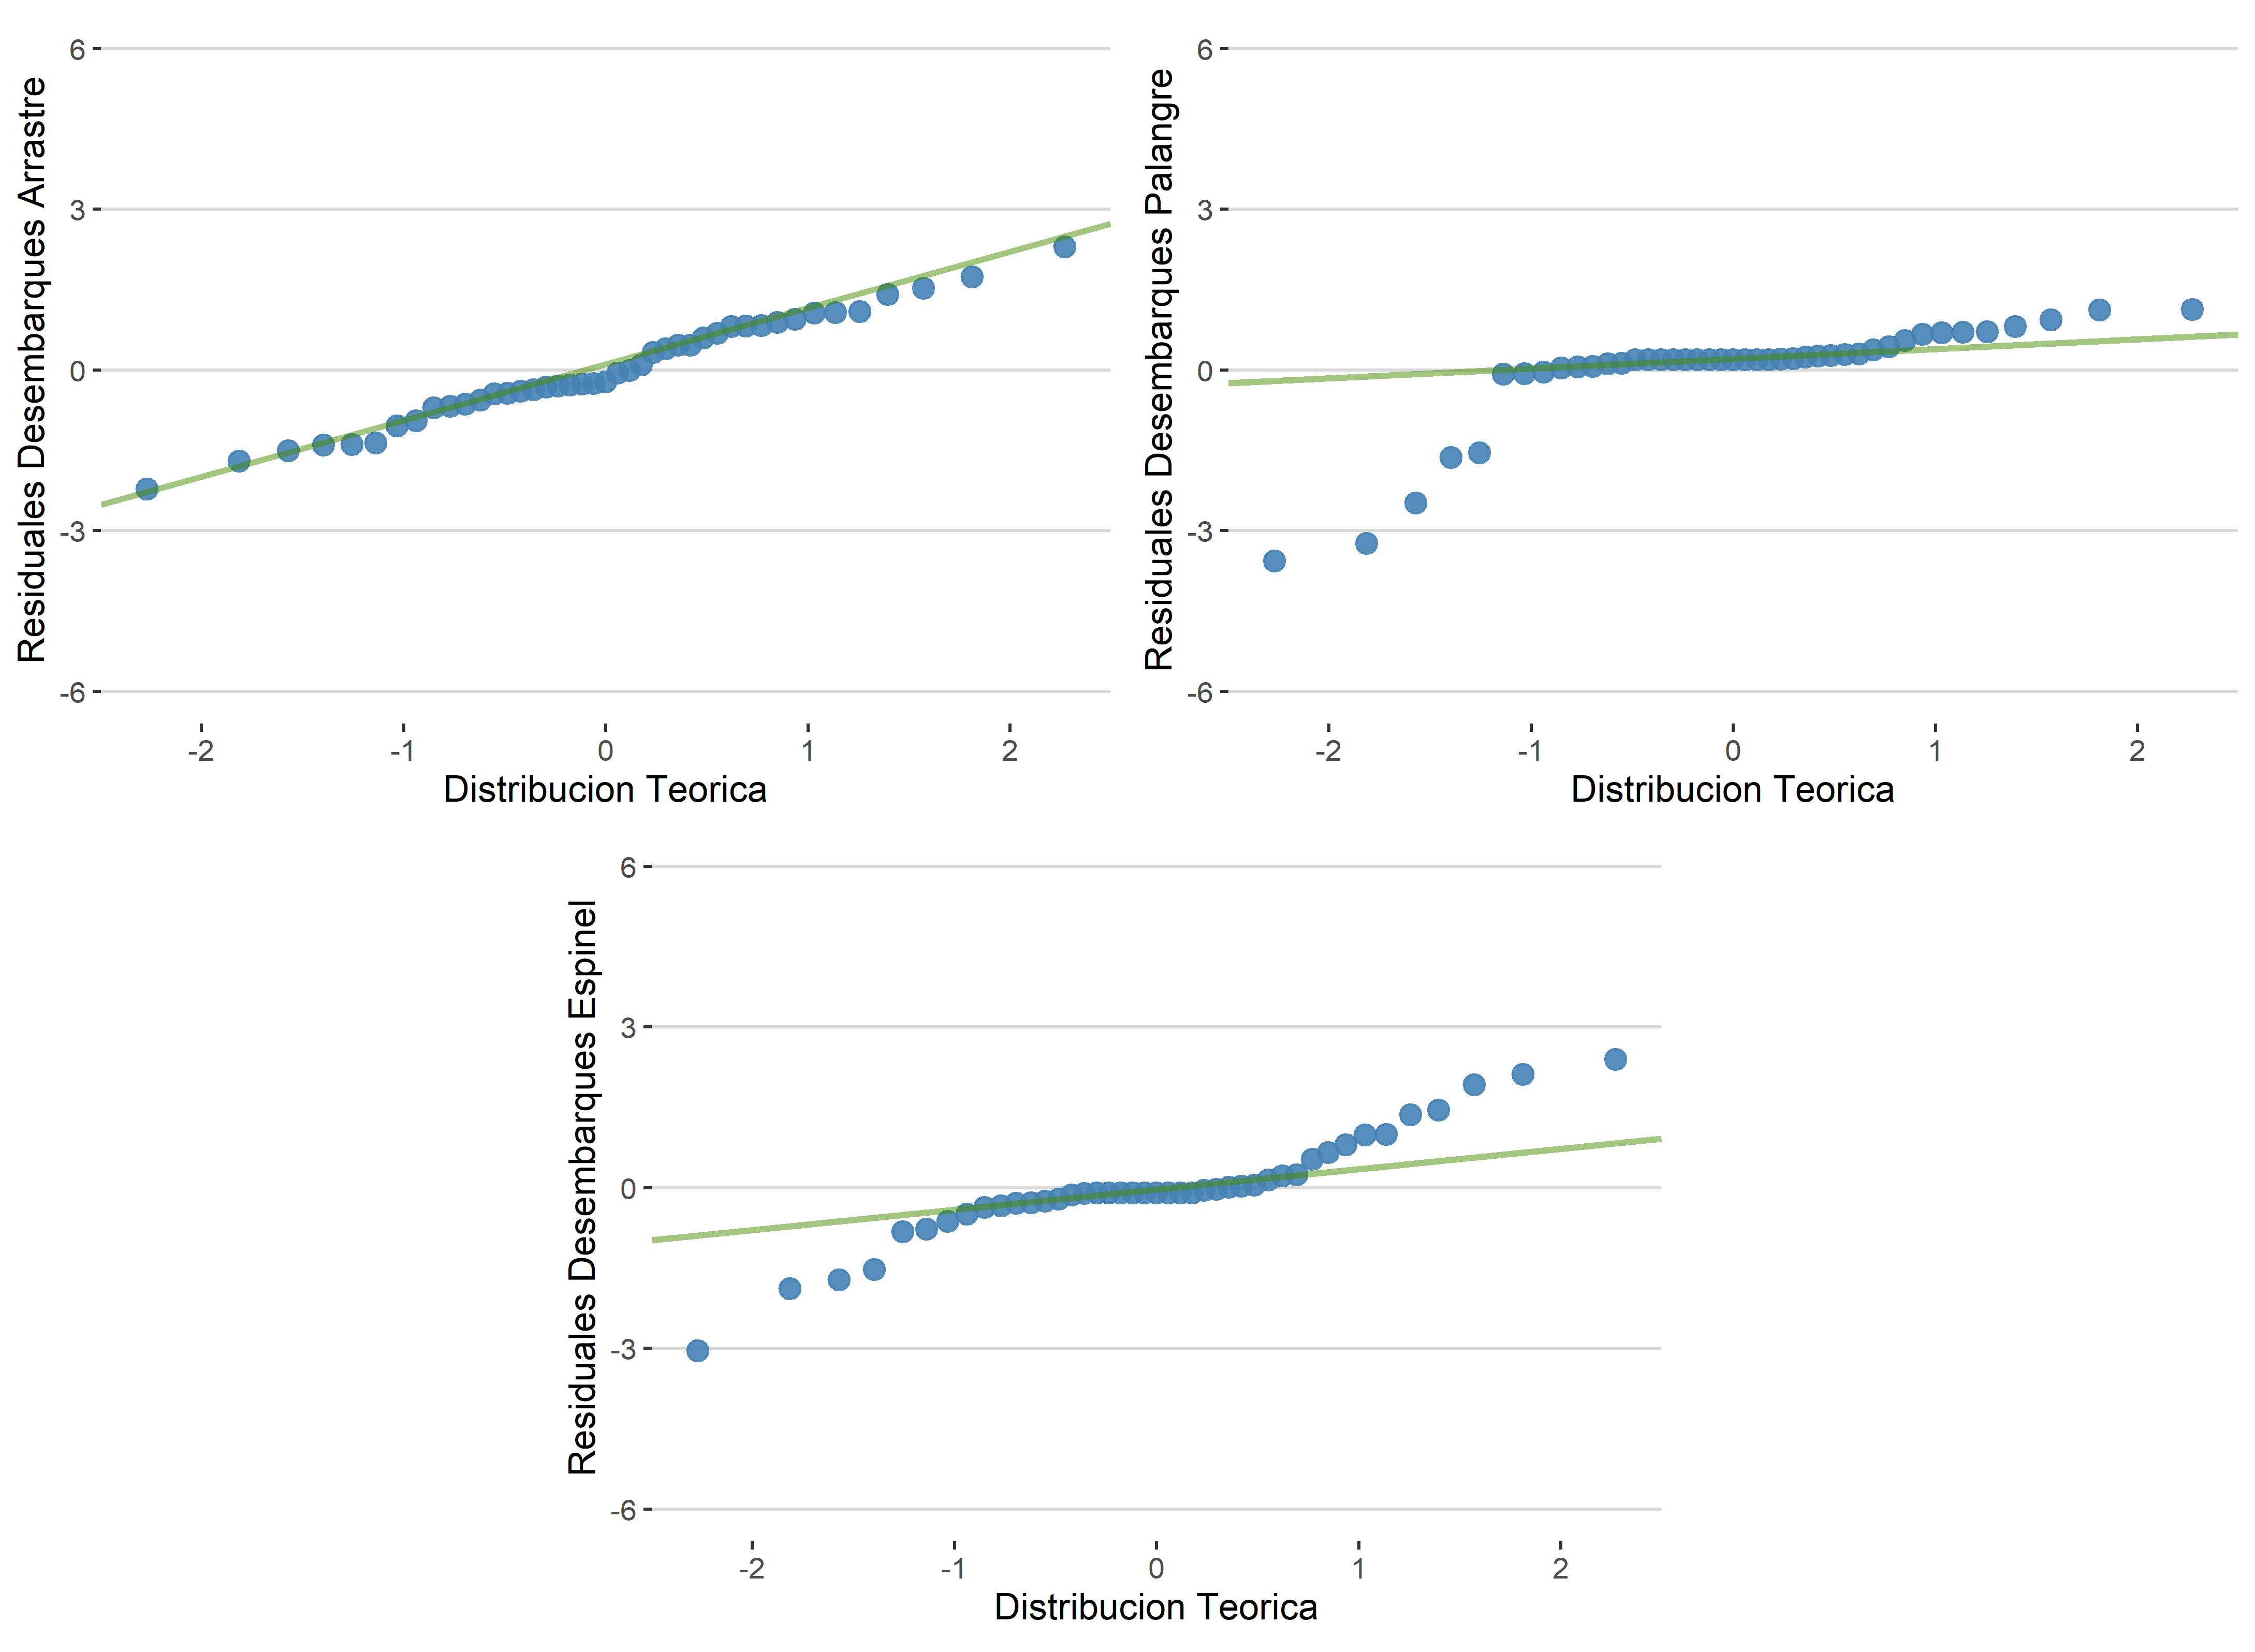
\includegraphics[width=0.8\textwidth]{Figuras/resid.yield.png}
\end{center}

\small \textbf{Figura 28}. Residuales de los datos de desembarque de las
flotas arrastrera, palangrera y artesanal, período 1977-2019.
\vspace{0.5cm} \normalsize

El ajuste a los datos de índices de abundancia por flota se presenta en
la Figura 29, con sus respectivos residuales por flota (Figura 30). Los
ajustes a las series temporales de abundancia son variables entre flotas
y crucero. En términos generales, se observa mejores ajustes en los
índices de abundancia de palangre y arrastre para el período 1, con una
menor precisión la flota artesanal y la biomasa desovante prospectada
durante los cruceros acústicos. Para el arrastre se observa un primer
período con una disminución de la CPUE hasta el año 1997 (cuadrante
izquierdo) y un posterior aumento durante el segundo período (cuadrante
derecho). El palangre presenta un período con valores máximos
(1998-2000) al igual que la flota artesanal (2001-2002).

\begin{center}
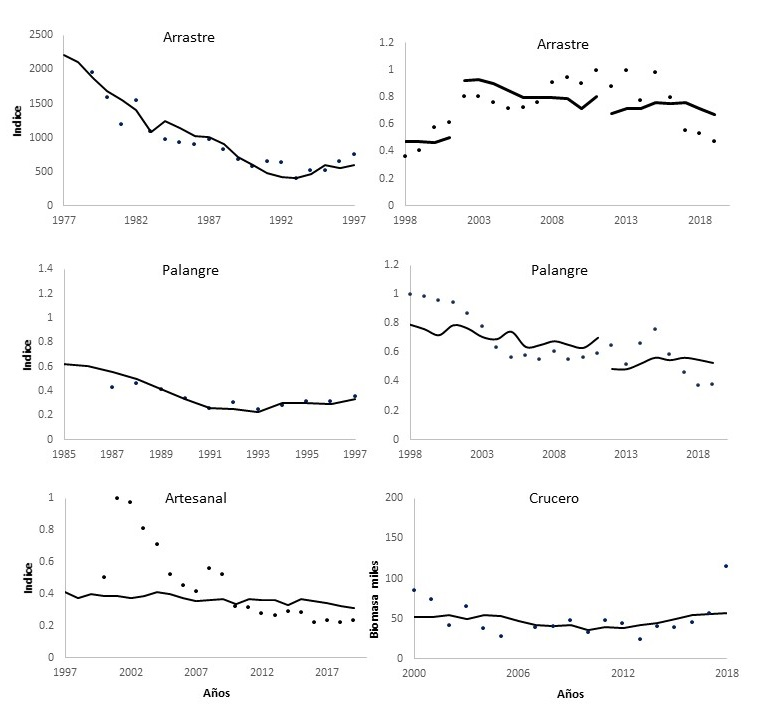
\includegraphics[width=0.8\textwidth]{Figuras/ajustes.png}
\end{center}

\small \textbf{Figura 29}. Índice de abundancia observado (puntos) y
estimado (línea continua) de las flotas arrastrera (kg/h.a.), palangrera
(kg/(nanz*h.r.)) y artesanal (kg/h.r.), junto a las predicciones del
crucero acústico. \vspace{0.5cm} \normalsize

\begin{center}
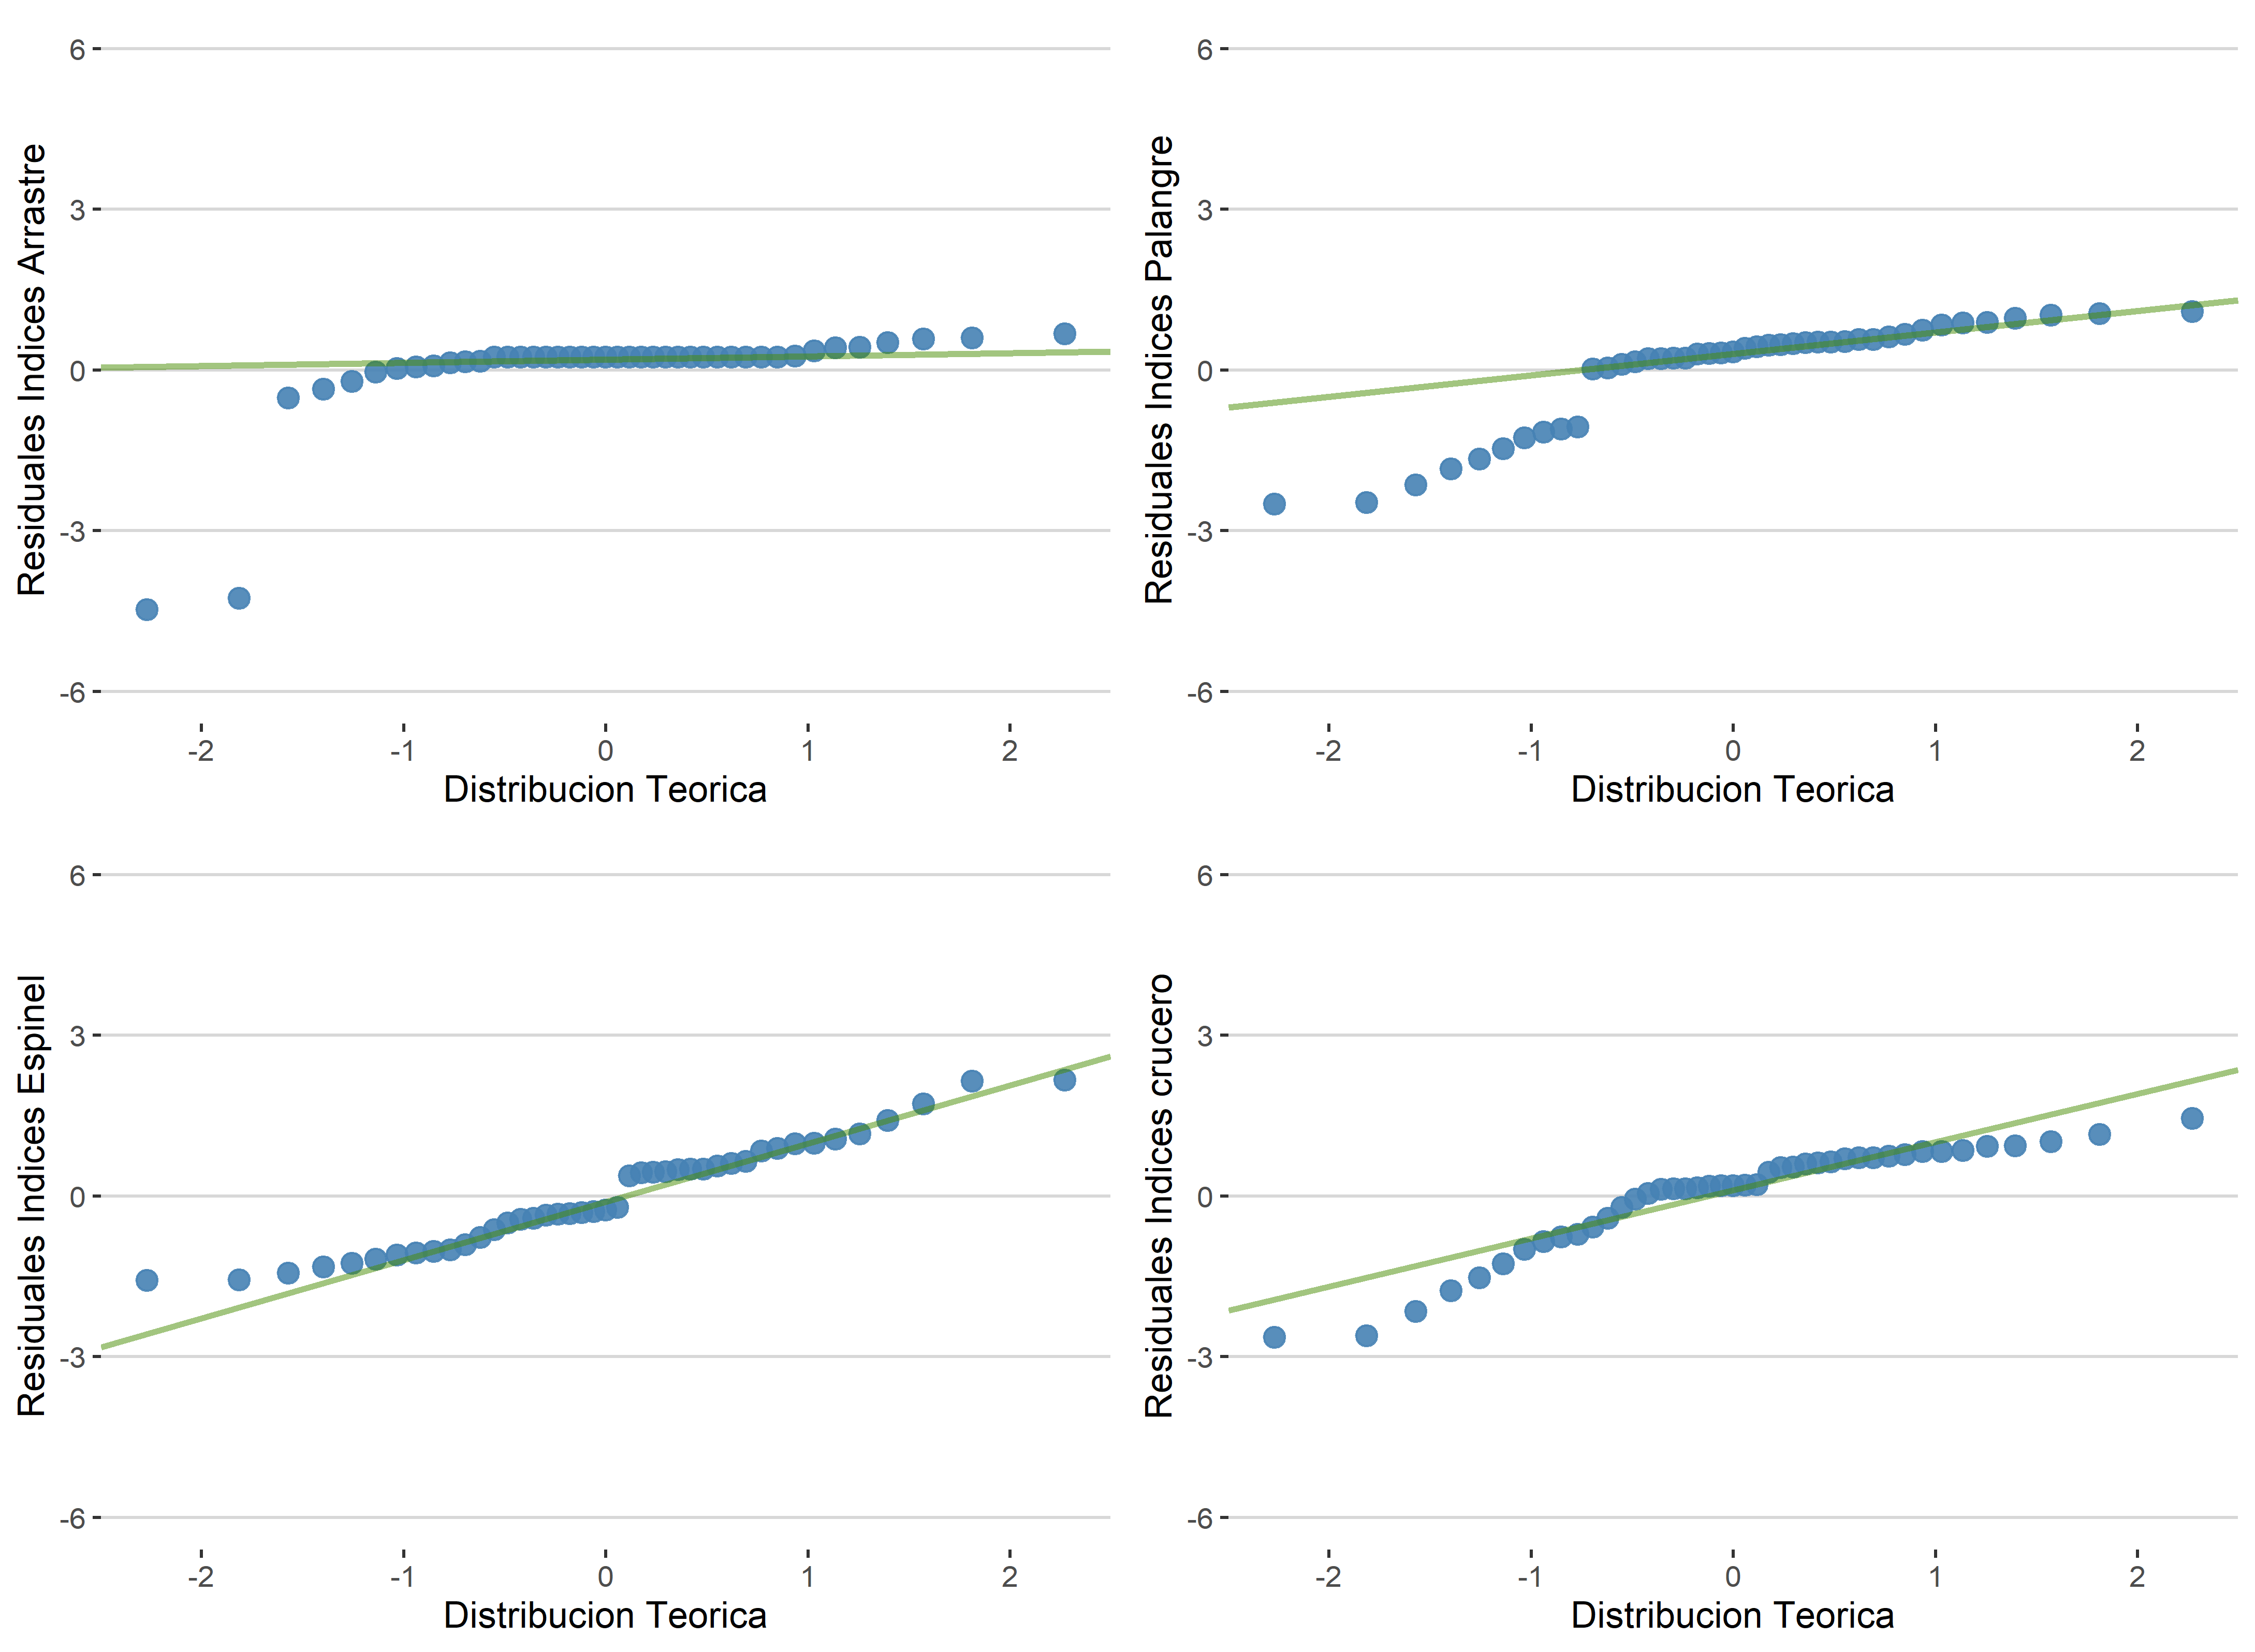
\includegraphics[width=0.8\textwidth]{Figuras/resid.ind.png}
\end{center}

\small \textbf{Figura 30}. Residuales índices de abundancia de la flota
arrastrera, palangrera, artesanal y crucero acústico. \vspace{0.5cm}
\normalsize

En la Figura 31 se observa la selectividad del arte de pesca para cada
flota, arrastre, palangre, espinel y crucero acústico. Las edades de
des-reclutamiento son de aproximadamente 18 años para el arrastre, 19
años para el palangre, 12 años en la flota artesanal y 21 para el
crucero acústico.

\begin{center}
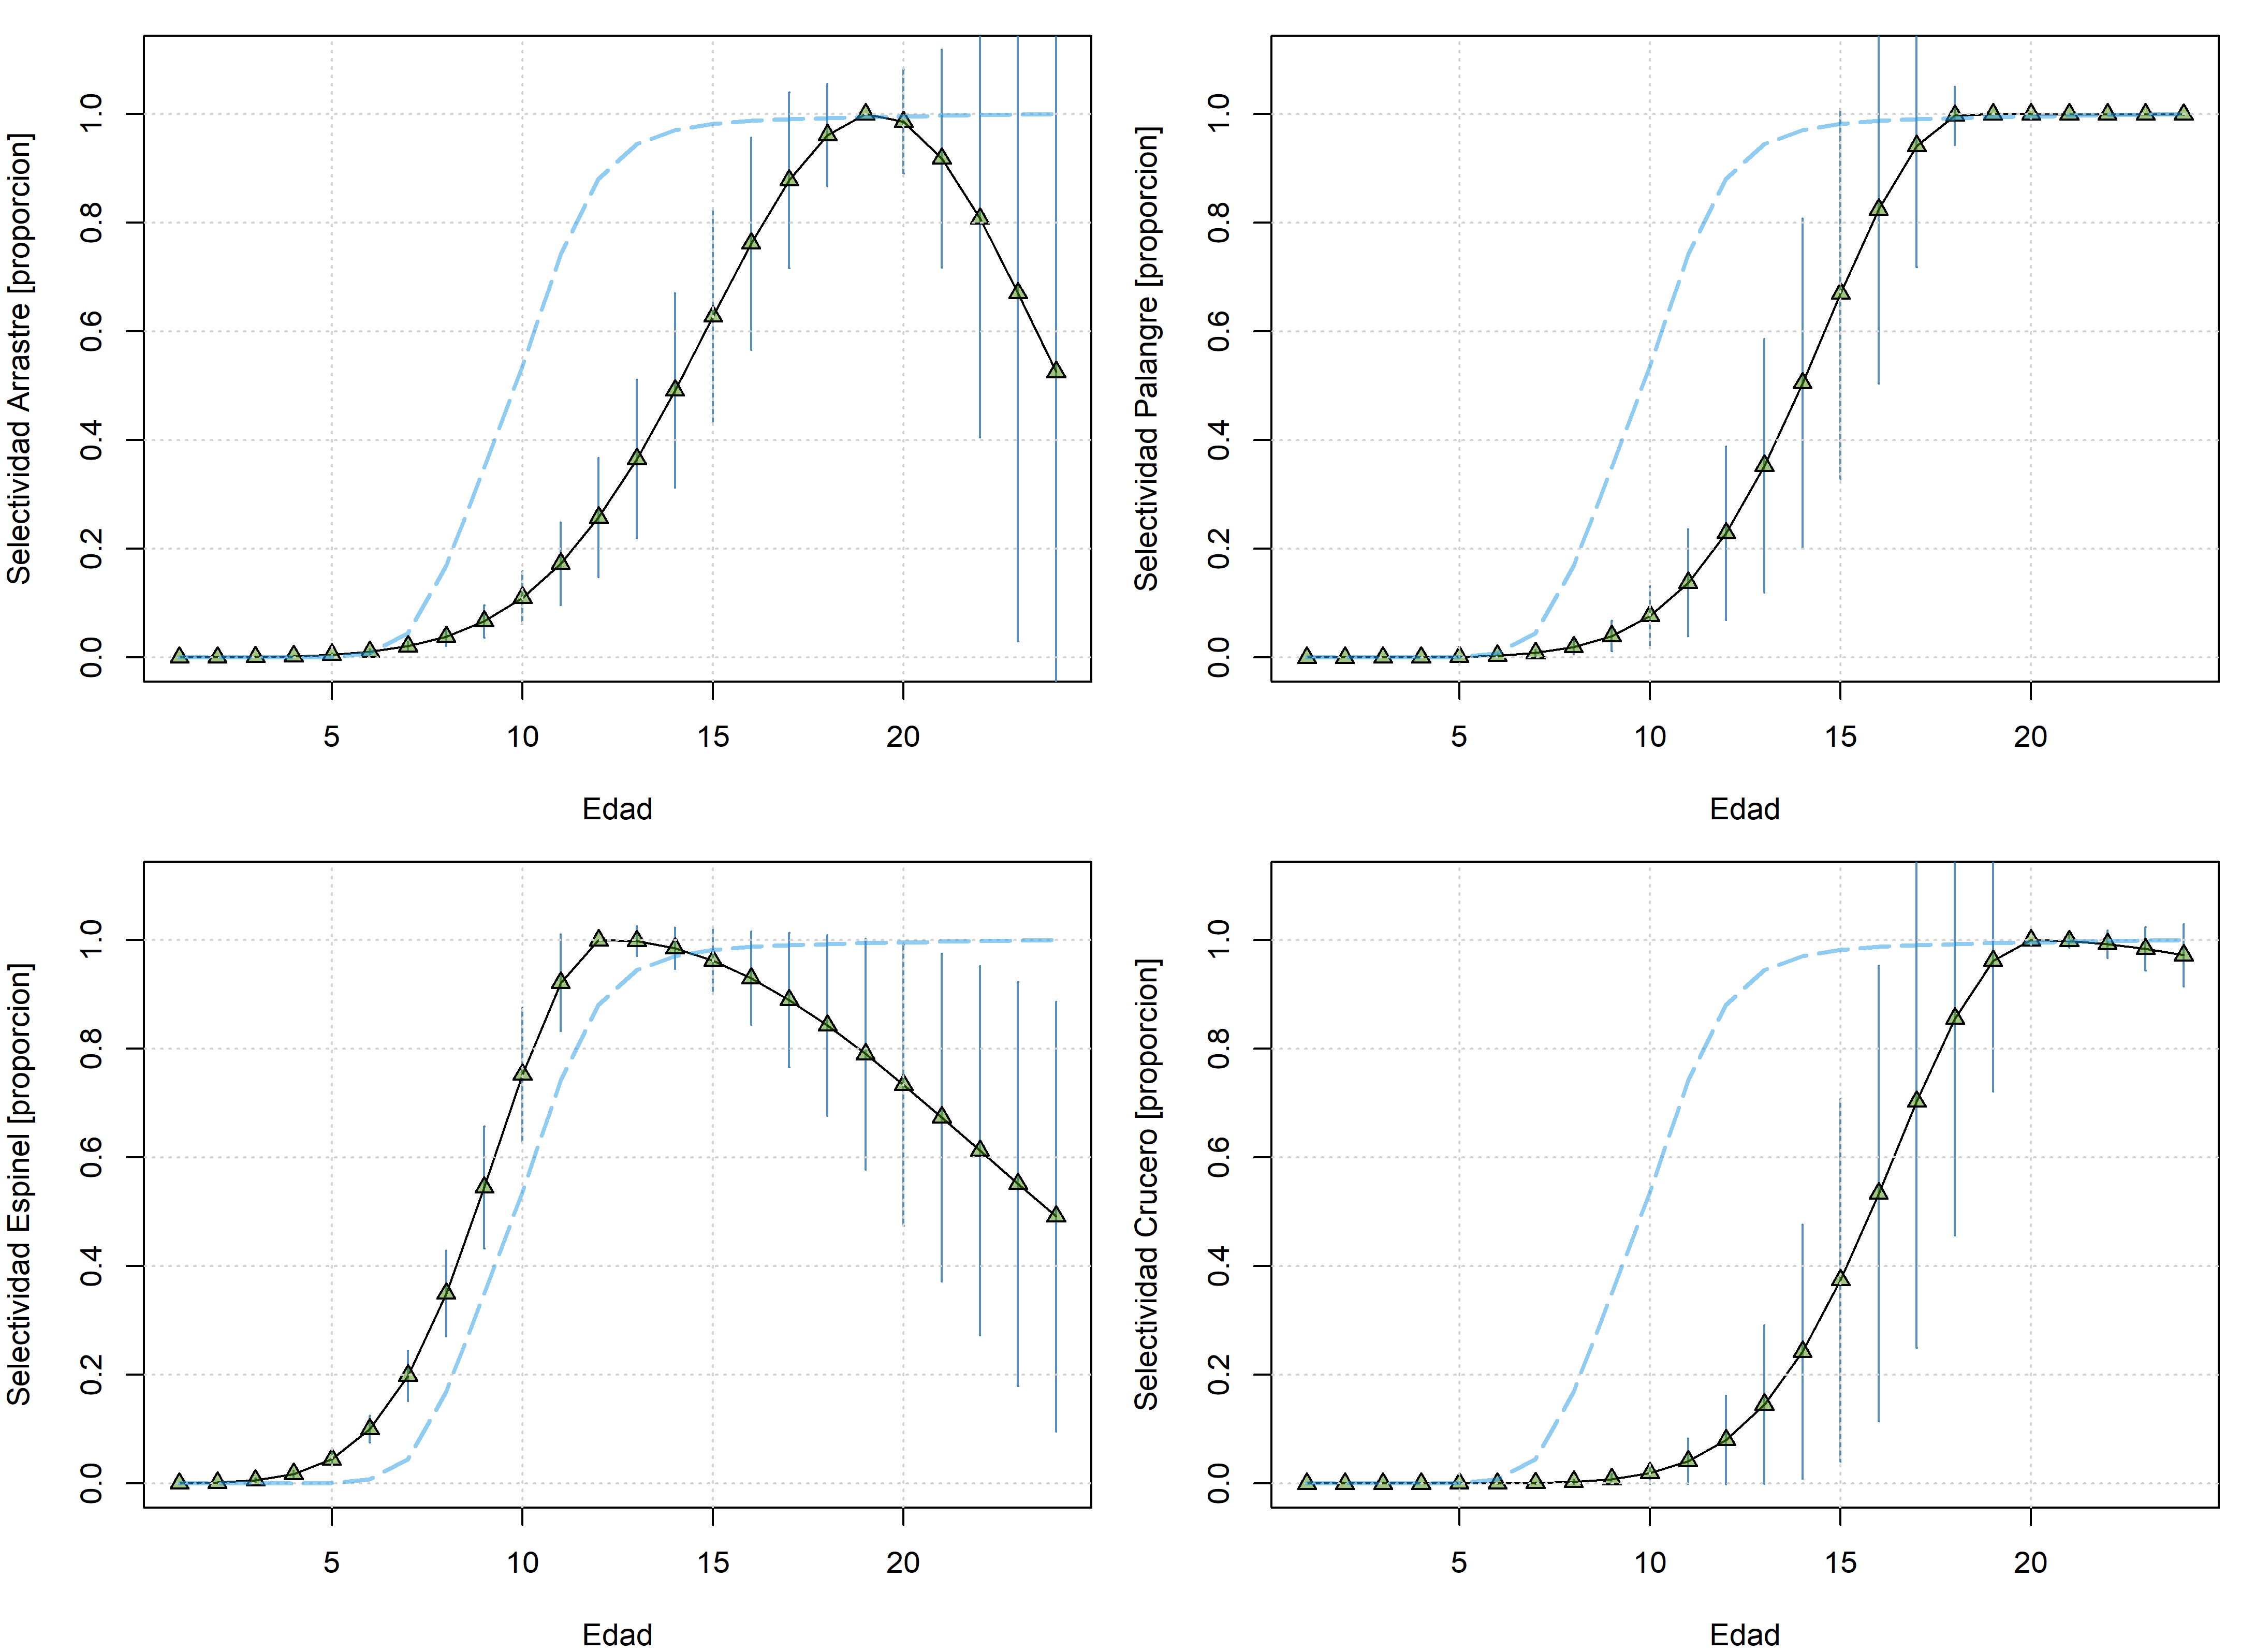
\includegraphics[width=0.8\textwidth]{Figuras/selectivities.png}
\end{center}

\small \textbf{Figura 31}. Selectividad de la flota arrastrera,
palangrera, artesanal y crucero acústico, en línea segmentada azul se
sobrepone la madurez sexual. \vspace{0.5cm} \normalsize

La mortalidad por pesca por flota y total se muestra en la Figura 32,
cómo ha sido recurrente los mayores niveles de mortalidad por pesca han
sido generados por la flota arrastrera. En magnitud le sigue la flota
palangrera, aunque durante los últimos 6 años esta flota mostró una
reducción importante en los niveles de remoción. En las tres flotas se
observa una significativa reducción de la mortalidad por pesca para el
año 2014, consecuencia de la reducción en las cuotas de captura. Con
respecto a la mortalidad total, se observa un aumento durante los
últimos 2 años generada principalmente por la flota arrastrera.

\begin{center}
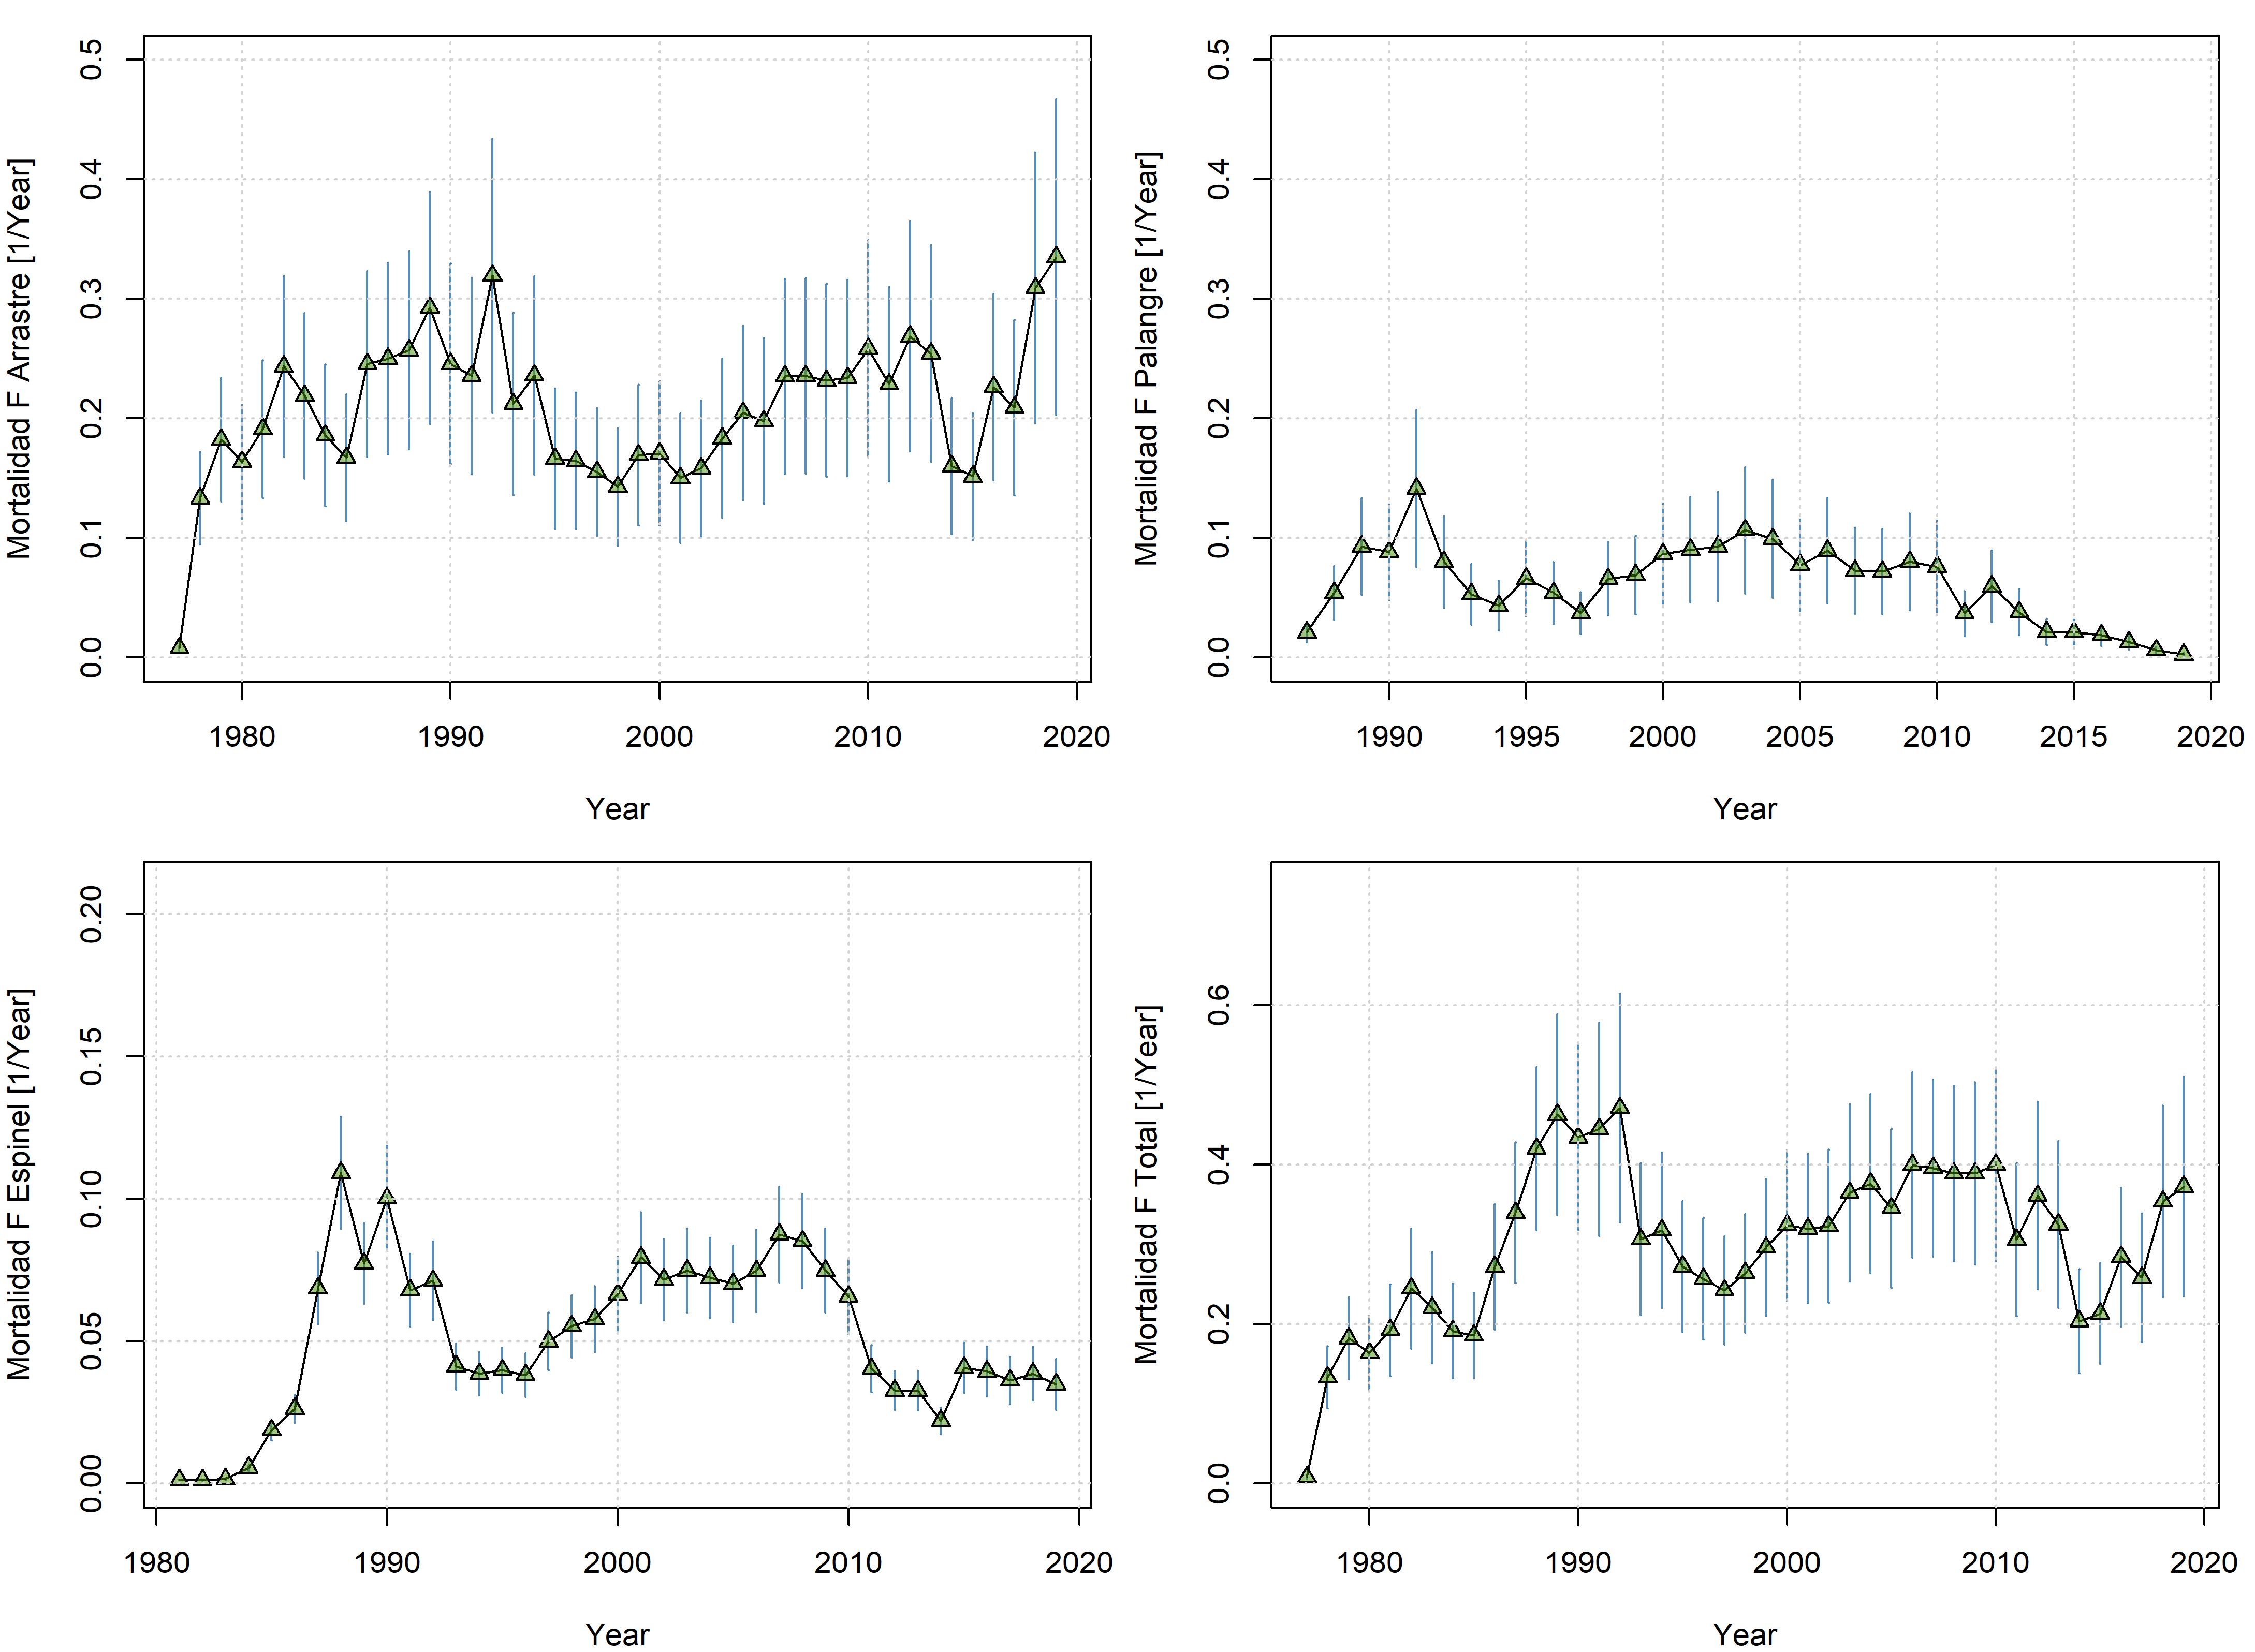
\includegraphics[width=0.8\textwidth]{Figuras/mortalidad.png}
\end{center}

\small \textbf{Figura 32}. Mortalidad por pesca estimada para la flota
arrastrera, palangrera, espinelera y mortalidad por pesca total.
\vspace{0.5cm} \normalsize

En cuanto a las estructuras de tallas, el arrastre presenta información
desde 1982 hasta 2018. Destacan los años 1982 y 1983 con estructuras que
poseen una importante participación de las edades mayores de 19 años,
las que no volvieron a aparecer con esa importancia en la historia de la
pesquería (Figura 33). Luego en 1986 y 1998 se aprecia un contingente de
peces de edades menores de 9 años, que sugieren un buen reclutamiento
asociado a los desoves del año 1982 y 1983. Desde el año 2001 hasta el
2007 se produce otro desplazamiento de la estructura hacia edades más
viejas. Finalmente, desde el 2008 la estructura se ha mantenido
relativamente estable con un pequeño aumento en la aparición de
ejemplares mayores a 19 años.

En el palangre (Figura 34) se observa la presencia de ejemplares de
mayor tamaño entre los años 1989-1992, desde el año 1995 y hasta 2000 la
estructura se mantiene relativamente estable, pero en durante el período
2001-2005 presenta un desplazamiento hacia edades más jóvenes. Desde el
año 2006 y hasta la actualidad es posible encontrar ejemplares
representando a las tallas mayores de la estructura, sobre todo los años
2015 al 2019 en donde se presenta un aumento importante en la proporción
de ejemplares entre 18 y 20 años.

Desde los residuales a la edad (Figura 35) se observa, para el período
1994-2005, una subestimación de ejemplares entre los 14 y los 19 y una
subestimación de ejemplares entre 6 y 12 años. Para el palangre, entre
los años 1990-1992 el modelo tiende a subestimar las tallas mayores a 13
años y sobrestimar tallas menores. Desde el año 1994 el modelo subestima
las tallas menores a 13 años y sobrestima las tallas mayores.

\begin{center}
\includegraphics[width=0.8\textwidth]{Figuras/FitAgeArrastre.png}
\end{center}

\small \textbf{Figura 33}. Ajuste estructuras de edades flota arrastrera
período 1981-2019, estimados (línea roja) y observados (barras) de la
proporción de edades en las capturas. \vspace{0.5cm} \normalsize

\begin{center}
\includegraphics[width=0.8\textwidth]{Figuras/FitAgeLongline.png}
\end{center}

\small \textbf{Figura 34}. Ajuste estructuras de edades flota palangrera
período 1989-2019, estimados (línea roja) y observados (barras) de la
proporción de edades en las capturas. \vspace{0.5cm} \normalsize

\begin{center}
\includegraphics[width=0.8\textwidth]{Figuras/Figura_35.png}
\end{center}

\small \textbf{Figura 35}. Residuales de estructura de edades de la
flota de arrastre y palangre. Subestimaciones (círculo azul) y
sobreestimaciones (círculo rojo), donde el tamaño corresponde a la
magnitud relativa del error por edad. \vspace{0.5cm} \normalsize

Para el espinel la estructura de edades abarca un rango de edades más
jóvenes que las flotas de arrastre y palangre (Figura 36), apareciendo
individuos a partir de los 3-4 años de edad. Los dos primeros años de
datos (1987 y 1988) corresponden a los años con grandes capturas
artesanales (20 a 30 mil t), pero luego no se dispone de datos para el
período 1989-1994, donde las capturas aún eran altas, pero con tendencia
a la baja. El período 1995-1999, se aprecia el desplazamiento de la
estructura hacia edades mayores. Desde 2000 hasta 2004 se observó una
estructura relativamente estable y desde 2005 a 2009 la participación de
edades jóvenes aumentó. En los últimos dos años de la serie no se
observan los ejemplares mayores a 17 años que habían sido observados en
el año 2017.

Los datos provenientes del crucero acústico muestran estabilidad los
primeros años para encontrar una ausencia de ejemplares menores a 10
años en 2011 (Figura 37). Es importante mencionar que la estructura de
edades presentada en este informe corresponde solo a ejemplares adultos,
obtenidos aplicando la ojiva de madurez macroscópica para cada sexo,
esto debido a la solicitud por parte de la Subsecretaría de Pesca y
Acuicultura de incorporar solo ejemplares adultos parte de la fracción
desovante y eliminar la fuerte presencia de ejemplares juveniles menores
a 7 años que se detectaron en los años 2016, 2017 y 2018.

Los residuales para la flota artesanal y los cruceros acústicos (Figura
38) se distribuyeron adecuadamente a través de los años y edades, con
algunos residuales positivos en las edades 3 a 6 en la segunda mitad de
los años ochenta, sin embargo, estos residuales no superan las 3
desviaciones estándar y por lo tanto están dentro del rango del 95\%.

\begin{center}
\includegraphics[width=0.8\textwidth]{Figuras/FitAgeArtesanal.png}
\end{center}

\small \textbf{Figura 36}. Ajuste estructuras de edades flota artesanal
período 1987-2019, estimados (línea roja) y observados (barras) de la
proporción de edades en las capturas. \vspace{0.5cm} \normalsize

\begin{center}
\includegraphics[width=0.8\textwidth]{Figuras/FitAgeCrucero.png}
\end{center}

\small \textbf{Figura 37}. Ajuste estructuras de edades fracción adulta
del crucero acústico período 2000-2019, estimados (línea roja) y
observados (barras) de la proporción de edades en las capturas.
\vspace{0.5cm} \normalsize

\begin{center}
\includegraphics[width=0.8\textwidth]{Figuras/Figura_38.png}
\end{center}

\small \textbf{Figura 38}. Residuales de estructura de edades de la
flota artesanal y crucero acústico. Subestimaciones (círculo azul) y
sobreestimaciones (círculo rojo), donde el tamaño corresponde a la
magnitud relativa del error por edad. \vspace{0.5cm} \normalsize

\hypertarget{comparaciuxf3n-escenarios-y-sensibilidad}{%
\subsection{4.1.4 Comparación escenarios y
sensibilidad}\label{comparaciuxf3n-escenarios-y-sensibilidad}}

Con el fin de observar de mejor forma los cambios en la incorporación
y/o modificación de la información se compara el modelo implementado en
la asesoría previa, 2019 con datos parciales mod0\_01 con el modelo
solicitado por el Comité Científico Técnico, que actualiza los datos al
2019 e incluye los pesos medios del crucero (mod0\_02) y flota
(mod0\_03). Finalmente, se incluyen dos configuraciones de sensibilidad
al modelo mod0\_03, la primera modifica los coeficientes de variación de
los índices de abundancia mod0\_03a (Tabla 3) y la segunda incluye un
cambio en la productividad de la población modificando el parámetro de
escarpamiento desde h=0.5 a h=0.75 mod0\_03b. En sombreado se destaca
modelo base.

\begin{center}
\includegraphics[width=0.8\textwidth]{Figuras/Figura_39.png}
\end{center}

\small \textbf{Figura 39}. (a) Biomasa desovante, (b) biomasa total, (c)
reclutamiento y (d) reducción de la biomasa desovante para los 5
escenarios periodo 1977-2019. \vspace{0.5cm} \normalsize

Las variables de estado biomasa desovante, total, reclutamiento y
reducción de la biomasa desovante se presentan en la Figura 40. En
términos de la reducción de la biomasa desovante (Figura 40,d), los
escenarios que muestran una mayor recuperación corresponden a los
mod0\_03a (BD/BD0=31\%) y mod0\_03b (BD/BD0=37\%), sin embargo, en todos
los escenarios la biomasa desovante disminuye durante los últimos 4
años. En el escenario mod0\_03b se observa un aumento en la biomasa
total al final de la serie (Figura 40,b), lo que se puede atribuir al
aumento en los reclutamientos desde el año 2010 debido al aumento en la
productividad de la población (Figura 40,c).

\begin{center}
\includegraphics[width=0.8\textwidth]{Figuras/Figura_40.png}
\end{center}

\small \textbf{Figura 40}. Mortalidad por pesca total para los 5
escenarios período 1977-2019. \vspace{0.5cm} \normalsize

El efecto de incluir los pesos medios del crucero acústico y de la flota
se puede observar en la Figura 41, en donde el ajuste de los escenarios
mod0\_01 (con pesos medios constantes) y mod0\_02 (con pesos medios del
crucero acústico) evidencia una tendencia suavizada, a diferencia de los
escenarios que incluyen los pesos medios de la flota (mod0\_03,
mod0\_03a y mod0\_03b), en los que el ajuste presenta una tendencia más
acerrada influenciada por la variación anual de los pesos medios en vez
de la utilización de valores constantes a los largo de la serie.

La captura se proyectó para los escenarios mod0\_3a y mod0\_03b
asumiendo para el año 2020 un valor desembarque igual a la CBA ponderada
por los respectivos valores de descarte y subreporte utilizados de forma
histórica en la evaluación de stock para cada flota, lo que entrega un
valor de desembarque 2020 incluyendo descarte y subreporte de 29600
toneladas (Figura 42). Los valores de CBA para los años 2021, 2022 y
2023 se reportan en la Tabla 18.

\begin{center}
\includegraphics[width=0.8\textwidth]{Figuras/Figura_41.png}
\end{center}

\small \textbf{Figura 41}. Índice de abundancia observado (puntos) y
estimado (línea continua) de las flotas arrastrera (1979-1997;
1998-2019) y palangrera (1987-1997; 1998-2019) para los 5 escenarios.
\vspace{0.5cm} \normalsize

\begin{center}
\includegraphics[width=0.8\textwidth]{Figuras/Figura_42.png}
\end{center}

\small \textbf{Figura 42}. Proyección de la captura para los años 2021,
2022 y 2023, cuadrante superior: mod0\_03a, cuadrante inferior:
mod0\_03b. \vspace{0.5cm} \normalsize

\hypertarget{anuxe1lisis-retrospectivo-1}{%
\subsection{4.1.5 Análisis
retrospectivo}\label{anuxe1lisis-retrospectivo-1}}

La Tabla 17, presenta los resultados en relación a la reducción de
información, en términos de parámetros, variables de estado y de calidad
de ajuste de la información (verosimilitud) para el modelo mod0\_03
(modelo que considera pesos medios por flota). En este sentido se
destaca la existencia de una importante congruencia en la estimación de
la biomasa virginal, la cual se re escala a niveles en cercanos en
relación a la reducción de información. El mismo efecto se aprecia
lógicamente en la estimación del reclutamiento virginal.

Tabla 17 Análisis retrospectivo, y sus implicancias en las variables de
estados y parámetros del modelo (mod0\_03).

El estimador del patrón retrospectivo (rho), resulta por lo tanto de
gran interés para poder comparar y realizar inferencia de la calidad del
modelo, y de cómo las variables se ven afectadas por la reducción de
información. La Figura 43, presenta el análisis retrospectivo del modelo
mod0\_03 de evaluación de stock de merluza del sur, mostrando el impacto
de la reducción de información de dos años de información prácticamente
no afecta las variables de estado. En términos de rho, se aprecia que la
reducción de información afecta y de manera negativa a la estimación de
la biomasa desovante (arreglar = -0,089) representando el mayor efecto
dentro de las variables evaluadas en términos de un patrón
retrospectivo). En el caso de los reclutamientos estos son alterados
positivamente (arreglar = 0,014), siendo esta variación de menor
cuantía. Finalmente, la variación de la mortalidad por pesca, presenta
niveles cercanos en torno a arreglar = 0,044.

\begin{center}
\includegraphics[width=0.8\textwidth]{Figuras/Figura_43.png}
\end{center}

\small \textbf{Figura 43}. Análisis retrospectivo del modelo de
evaluación de stock y su efecto en la biomasa desovante, el
reclutamiento y la mortalidad (mod0\_03). \vspace{0.5cm} \normalsize

La Tabla 18 muestra el desempeño del análisis retrospectivo del modelo
mod0\_03b. En donde se destaca, y al igual al caso anterior, el modelo
presenta una importante sintonía en la reducción de información y de su
efecto es la condición inicial del stock. Lo anterior se puede observar
que la estimación de la biomasa desovante virginal tiene una variación
menor, incluso con una diferencia de 5 años de la condición estimada en
completitud de información. Con respecto al reclutamiento virginal y a
los parámetros de la relación stock recluta, se confirma la mínima
variación registrada entre escenarios analizados.

Tabla 18 Análisis retrospectivo, y sus implicancias en las variables de
estados y parámetros del modelo (mod0\_03b).

La Figura 44, presenta el análisis retrospectivo del modelo mod0\_03b de
evaluación de stock de merluza del sur, mostrando el impacto de la
reducción de información de dos años de información prácticamente no
afecta de manera importante la biomasa desovante. En términos de rho, se
aprecia que la reducción de información afecta levemente y de manera
negativa a la estimación de la biomasa desovante (arreglar = -0,062). En
el caso de los reclutamientos estos son alterados en torno a arreglar =
0,056, representando junto a la biomasa desovante las variables que
mostraron un mayor impacto de la reducción de información de las
variables evaluadas, en términos de un patrón retrospectivo. Finalmente,
la variación de la mortalidad por pesca parece de menor cuantía, por
solo presentar niveles cercanos a cero (arreglar = 0,034).

\begin{center}
\includegraphics[width=0.8\textwidth]{Figuras/Figura_44.png}
\end{center}

\small \textbf{Figura 44}. Análisis retrospectivo del modelo de
evaluación de stock y su efecto en la biomasa desovante, el
reclutamiento y la mortalidad (mod0\_03b). \vspace{0.5cm} \normalsize

La Figura 45 muestra el impacto de la reducción de información en la
reducción poblacional, contrastada en ambos casos de estudio. En esta
figura se puede observar, que el modelo mod0\_03 muestra una leve
subestimación al reducir la información con la cual se realiza la
evaluación poblacional. En efecto como se mostró anteriormente, el
patrón retrospectivo en este caso es negativo lo que produce una
estimación si bien en torno a la condición actual del recurso, está en
cada resta de información parece ser de menor cuantía. Por otro lado, en
el caso del modelo mod0\_03b, el cual se caracteriza por presentar una
condición de productividad mayor al caso anterior, permite estimar
niveles más cercanos al 40\% de agotamiento del BD/BDo. En relación a el
patrón retrospectivo para este escenario, podemos comentar que si bien
el cambio relativo de BD es de menor error que el calculado para el caso
mod0\_03, persiste el mismo patrón que estima menores niveles de
agotamiento en cada reducción de información.

\begin{center}
\includegraphics[width=0.8\textwidth]{Figuras/Figura_45.png}
\end{center}

\small \textbf{Figura 45}. Análisis retrospectivo del modelo de
evaluación de stock y su efecto en la reducción poblacional (BD/BDo).
\vspace{0.5cm} \normalsize

\hypertarget{objetivo-especuxedfico-2-1}{%
\subsection{4.2. Objetivo específico
2:}\label{objetivo-especuxedfico-2-1}}

\emph{``Determinar las variables poblacionales de los recursos pesqueros
en estudio conforme al marco legal vigente y estimar el valor de los
Puntos Biológicos de Referencia, determinados por los Comités Científico
y Técnicos (CCT) respectivos, bajo condiciones de incertidumbre
estructural y de estimación empleando el mejor conocimiento e
información disponible a la fecha de ejecución del estudio.''}

\hypertarget{variables-de-estado-y-biomasa-modelo0_03a}{%
\subsection{4.2.1 Variables de estado y biomasa
Modelo0\_03a}\label{variables-de-estado-y-biomasa-modelo0_03a}}

En la Tabla 19 se presentan los valores de las variables de estado
biomasa total, desovante y juvenil, además del número de reclutas y la
mortalidad por pesca anual estimadas por el modelo de evaluación base.
Para el año 1977 se estima una biomasa total de 1064 mil toneladas y una
biomasa desovante de 444 mil toneladas. Para el año 1977 se estima una
biomasa total de 1106 mil toneladas y una biomasa desovante de 454 mil
toneladas. Para el año 2019 las estimaciones indican una biomasa total
aproximada de 536 mil toneladas y una biomasa desovante de 141 mil lo
que corresponde aproximadamente a un 31\% de reducción (Figura 46). Las
tendencias en el agotamiento de la biomasa desovante (Figura 46)
muestran una disminución progresiva hasta el año 2001 y alcanzando el
punto objetivo en el año 1991. Se mantiene durante los siguientes 13
años en torno a un 32\% para disminuir nuevamente durante los últimos 4
años. La biomasa total va en declive desde el año 2000 alcanzando
actualmente un 48\% de reducción.

\begin{center}
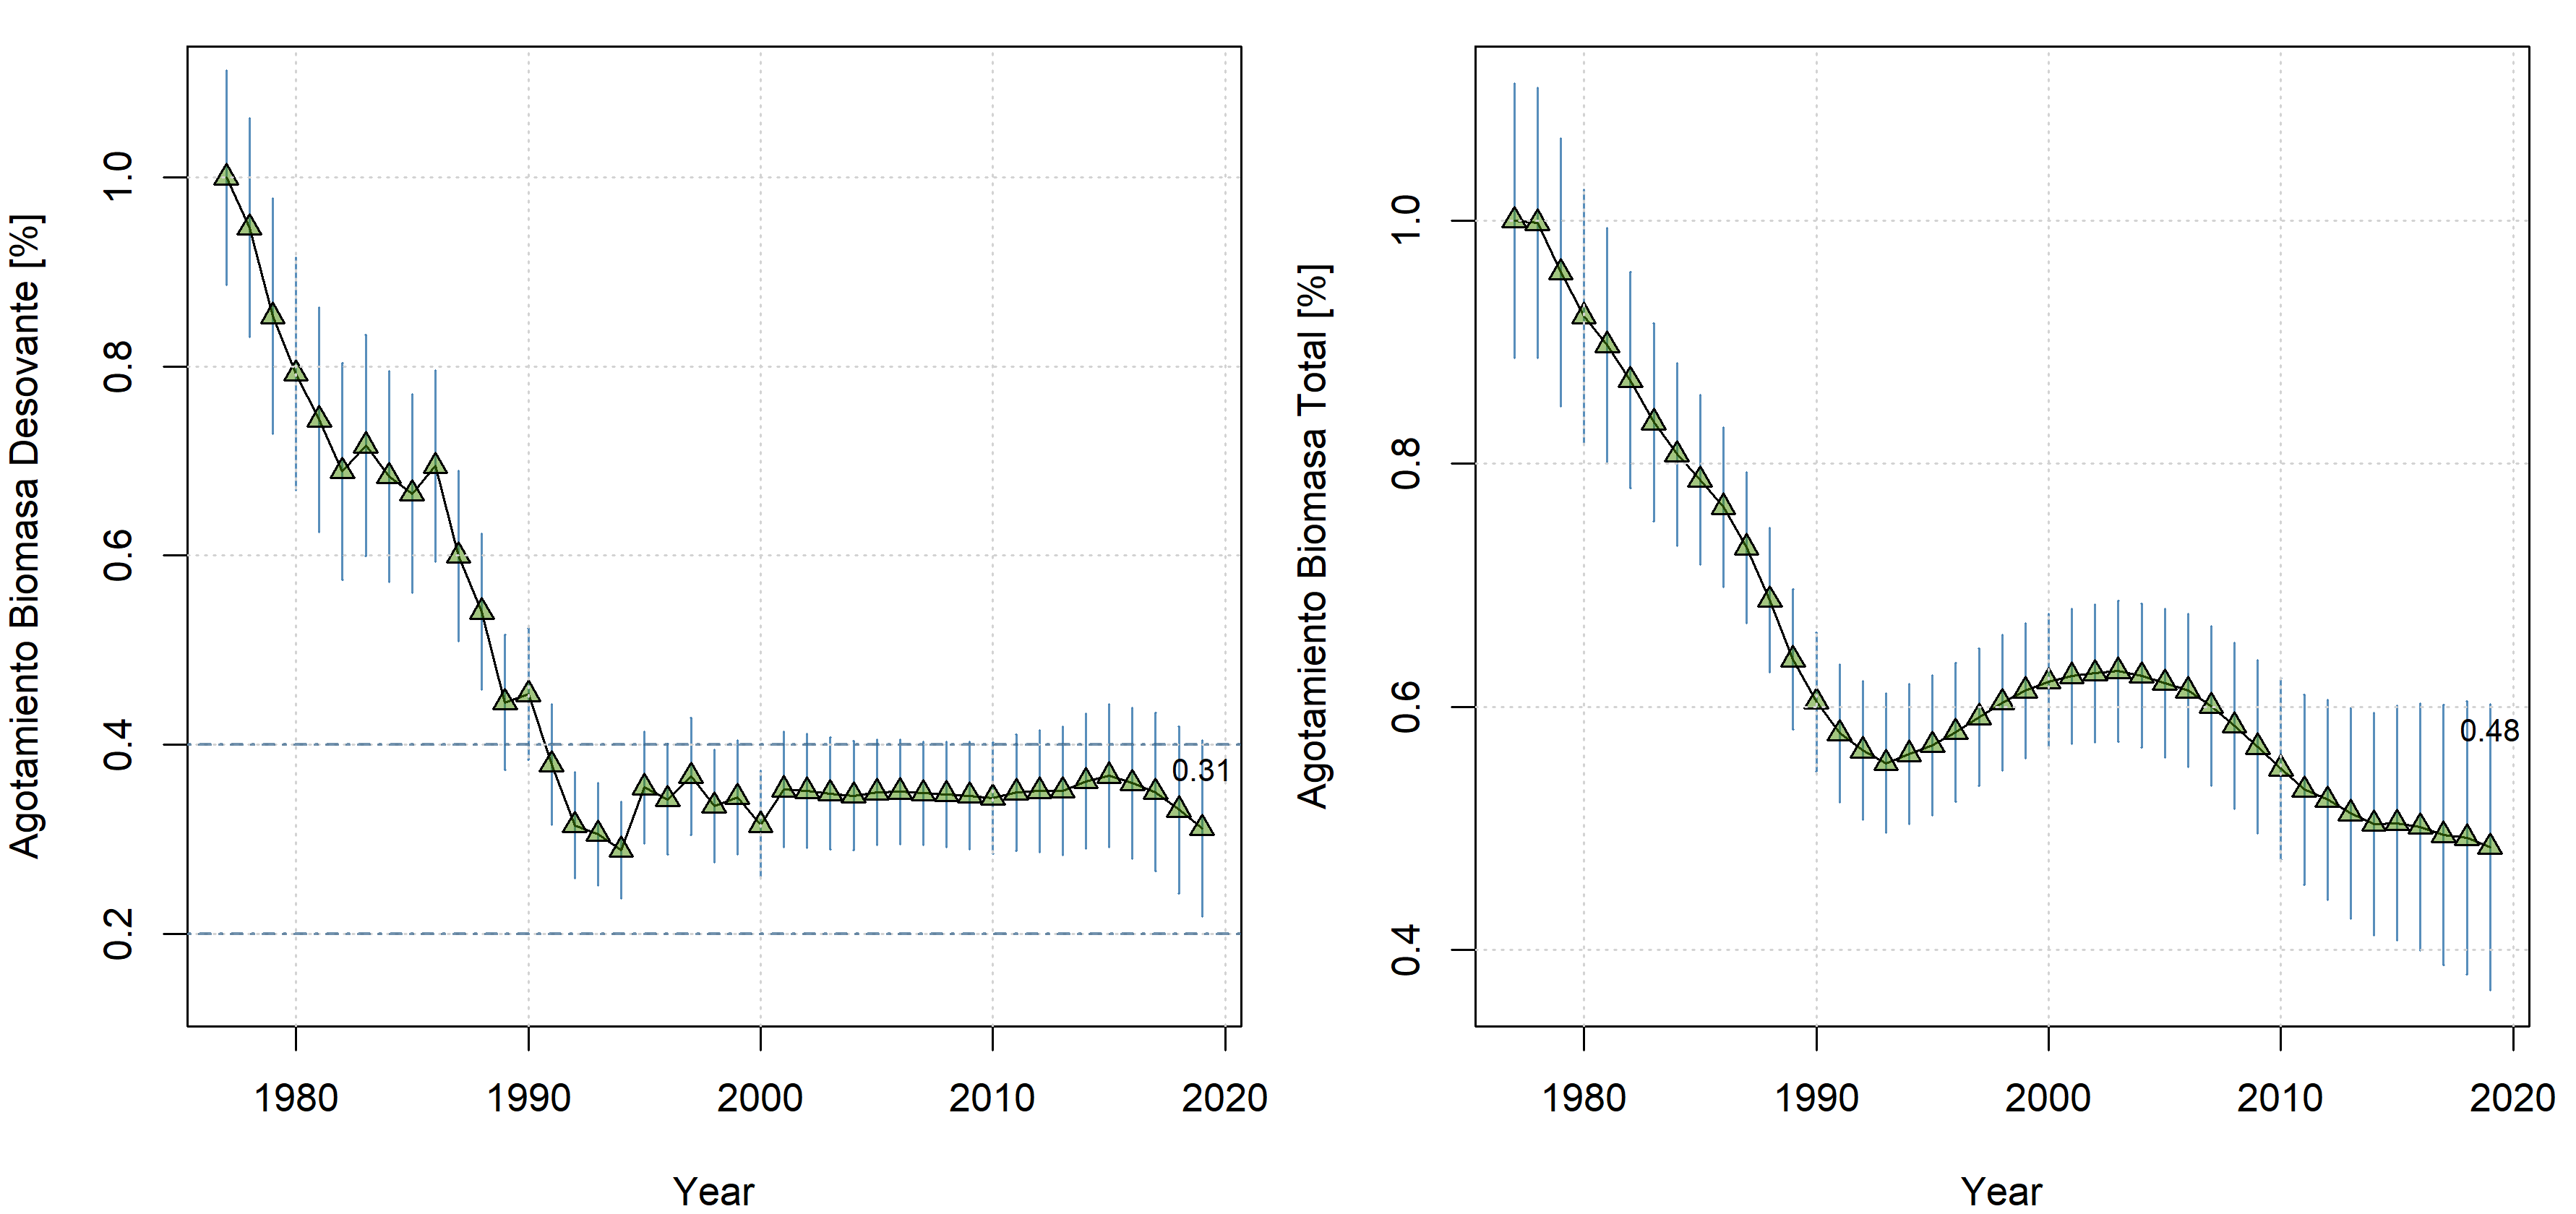
\includegraphics[width=0.8\textwidth]{Figuras/depletion.SB_BT.png}
\end{center}

\small \textbf{Figura 46}. Reducción de la biomasa desovante en
porcentaje (BD/BDO) y biomasa total en porcentaje período 1977-2019.
\vspace{0.5cm} \normalsize

Tabla 19 Variables de estado biomasa total (BT), desovante (BD) y
juvenil (B6) en miles de toneladas, reclutas (R) en número y mortalidad
por pesca anual (FT) obtenidas del ajuste del modelo base.

El reclutamiento estimado se presenta en la Figura 47, durante los
primeros 20 años el reclutamiento se mantiene aproximadamente en los 150
millones de individuos para luego descender hasta el año 2010 a 98
millones de individuos. Desde el año 2010 y hasta el 2018 se observa un
leve aumento de los reclutamientos hasta alcanzar el orden de 110
millones de individuos.

\begin{center}
\includegraphics[width=0.8\textwidth]{Figuras/Figura_47.png}
\end{center}

\small \textbf{Figura 47}. Reclutamiento (millones de individuos)
estimado por el modelo base para el período 1977-2019. \vspace{0.5cm}
\normalsize

\hypertarget{estatus-y-puntos-bioluxf3gicos-de-referencia}{%
\subsection{4.2.2 Estatus y Puntos Biológicos de
Referencia}\label{estatus-y-puntos-bioluxf3gicos-de-referencia}}

La reducción de la biomasa desovante se muestra en la Figura 48,
comenzando con una condición de subexplotación a inicios del período.
Luego, los altos niveles de captura aplicados hasta los 90´s produjeron
una disminución abrupta del potencial reproductivo de la población,
sobre pasando en 1991 el punto biológico objetivo. Al año 2019 la
merluza del sur se encuentra en un 31\% de la condición inicial.

El estado actual de esta pesquería es de sobreexplotación y sobrepesca,
con un valor de FRMS de 0.257 año-1 y de mortalidad por pesca al 2019 de
0.372 año-1.

\begin{center}
\includegraphics[width=0.8\textwidth]{Figuras/kobe_plot.png}
\end{center}

\small \textbf{Figura 48}. Diagrama de fases merluza del sur período
1977-2019, FRMS=0,257 año-1. \vspace{0.5cm} \normalsize

\hypertarget{objetivo-especuxedfico-3-1}{%
\subsection{4.3. Objetivo específico
3:}\label{objetivo-especuxedfico-3-1}}

\emph{``Analizar las distintas alternativas de Captura Biológicamente
Aceptable para estos stocks acorde con las estrategias de explotación y
reglas de control previamente definidas y considerando los posibles
estados de la naturaleza, con sus respectivos análisis de riesgo,
incluyendo análisis en horizontes de mediano y largo plazo, según
requerimiento.''}

\hypertarget{cba-2021-2023}{%
\subsection{4.3.1 CBA 2021-2023}\label{cba-2021-2023}}

La Tabla 20 muestra la CBA estimada para los años 2021, 2022 y 2023 bajo
diferentes niveles de riesgo (10-50\%) y bajo diferentes escenarios de
evaluación. Para el año 2020 se asumió un desembarque igual a la CBA
establecida para el año en curso, ponderada por los valores de descarte
y subreporte utilizados históricamente en la evaluación de stock para
cada flota. Es importante tener en consideración que para el cálculo de
la CBA proyectada para los años 2022 y 2023 no fue posible incluir este
ponderador de descarte y subreporte.

Tabla 20 Captura Biológicamente Aceptable (CBA) para diferentes
ponderadores de FRMS bajo una estrategia de explotación con mortalidad
por pesca constante. Se evaluaron los riesgos entre 50\% y 10.

\hypertarget{objetivo-especuxedfico-4-1}{%
\subsection{4.4. Objetivo específico
4:}\label{objetivo-especuxedfico-4-1}}

\emph{``Desarrollar los lineamientos técnicos e implementar la
aproximación de Evaluación de Estrategias de Manejo (EEM).''}

\hypertarget{definiendo-reglas-de-control-de-captura}{%
\subsection{4.4.1 Definiendo reglas de control de
captura}\label{definiendo-reglas-de-control-de-captura}}

Como parte de los lineamientos técnicos asociados con la implementación
de los procesos de Evaluación de Estrategias de Manejo (EEM) en merluza
del sur, se definió un conjunto de PM que incorporan diferentes opciones
de Reglas de Control de Capturas (RCC), plausibles umbrales para los PBR
y varios niveles de productividad de la población.

El acercamiento implementado en este objetivo está orientado a comparar
diferentes PM bajo la premisa que la información que alimenta el MEP en
cada año de iteración proviene de información perfecta deriva de un
modelo operativo (MO). El proceso de comparación de PMs es un análisis
multidimensional debido a las múltiples opciones que derivan de la
combinación de RCC, PBR y niveles de productividad. Por ejemplo, para
este ejercicio se definieron cuatro niveles de PBR (BDRMS=\{0.4, 0.3\},
BDLIM=\{0.2\}, FRMS=\{45\%bdpr\}), dos estrategias de explotación
alternativas basadas en capturas y tasas de explotación constantes, tres
niveles umbrales de captura y mortalidad por pesca la cuales son
anexadas a los PBR, y finalmente, cuatro niveles de productividad
(reclutamientos fijos alto y bajos, reclutamientos afectos a desvíos
aleatorios bajo umbrales altos y bajos). La combinación de todos estos
elementos en diferentes PMs envuelve un extenso proceso de simulación
que es altamente demandante de cálculos computacionales.

La Figura 49 muestra las proyecciones de doce PMs (cada panel) que
combinan parte de los elementos indicados en el párrafo anterior. En una
primera inspección de resultados se observan diferencias importantes
derivadas de los supuestos de productividad (columnas), y en una segunda
medida debido a la utilización de los PBRs en la configuración de cuatro
RCC (filas). Si bien, las diferencias no son evidentes en términos de
biomasa, la Figura 50 muestra que los niveles de captura en cada PM son
altamente sensibles a la RCC utilizada (filas), mientras que los niveles
de incertidumbre parecen responder a los supuestos de productividad
(columnas).

De acuerdo a los PM evaluados, se observa que solo las proyecciones
basadas en reclutamientos afectos a desvíos aleatorios permiten en
algunos años alcanzar el objetivo de manejo definido por el PBR DBRMS
(Figura 51). En efecto, ninguno de los escenarios con reclutamientos
fijos (ya sean altos o bajos) permite una recuperación de la biomasa
desovante mayor a un 40 de la biomasa virginal.

\begin{center}
\includegraphics[width=0.8\textwidth]{Figuras/Figura_49.png}
\end{center}

\small \textbf{Figura 49}. Proyecciones de la biomasa desovante bajo
doce procedimientos de manejo que combinan diferentes niveles de
productividad y opciones de PBR. \vspace{0.5cm} \normalsize

\begin{center}
\includegraphics[width=0.8\textwidth]{Figuras/Figura_50.png}
\end{center}

\small \textbf{Figura 50}. Proyecciones de la captura bajo doce
procedimientos de manejo que combinan diferentes niveles de
productividad y opciones de PBR. \vspace{0.5cm} \normalsize

\begin{center}
\includegraphics[width=0.8\textwidth]{Figuras/Figura_51.png}
\end{center}

\small \textbf{Figura 51}. Proyecciones del nivel de agotamiento bajo
doce procedimientos de manejo que combinan diferentes niveles de
productividad y opciones de PBR. \vspace{0.5cm} \normalsize

La Figura 52 muestra un resumen de las principales medidas de desempeño
como la razón entre la biomasa proyectada y la biomasa virginal, la
captura media en la proyección, la variación de la captura anual bajo
una ventana móvil de 5 años, y un conjunto de riesgos recurrentemente
utilizado para definir umbrales ce captura.

Estas medidas de desempeño tienen como objetivo resguardar diferentes
intereses. Por ejemplo, la probabilidad que la biomasa proyectada sea
menor que la biomasa objetivo definida por el PBR BDRMS, representa una
componente conservacionista que no considera ningún elemento operacional
de las flotas de pesca. Mientras que la variabilidad de la captura en
una base de 5 años, busca resguardar la estabilidad de pesquería en
términos de evitar cambios inter-anuales en la renta de la flota en un
corto plazo.

\begin{center}
\includegraphics[width=0.8\textwidth]{Figuras/Figura_52.png}
\end{center}

\small \textbf{Figura 52}. Ejemplo de medidas de desempeño para un
conjunto de PMs que incluyen opciones de reclutamiento y dos reglas de
control de captura. \vspace{0.5cm} \normalsize

La combinación entre las diferentes medidas de desempeño es la mejor
opción para comparar entre PM. Por lo tanto, el siguiente paso en los
análisis es realizar una evaluación cruzada de estas medidas de
desempeño con objeto de identificar las mejores combinaciones de PM que
permitan balancear objetivos conservacionistas, económicos y
posiblemente sociales.

\hypertarget{ordenando-y-visualizando-resultados}{%
\subsection{4.4.2 Ordenando y visualizando
resultados}\label{ordenando-y-visualizando-resultados}}

Debido a los múltiples resultados y opciones derivados de la evaluación
de procedimiento de manejo, uno de los desafíos de este proceso es la
adecuada comunicación a los usuarios de las diferentes opciones que
garanticen el balance de los intereses involucrados (económicos,
conservación, social, etc). Como parte de la aproximación a la
Evaluación de Estrategias de Manejo (EEM), se desarrolló una interfase
de comunicación para exponer los resultados de la sección anterior.

La Figura 53 muestra el tablero inicial de esta interfase que permite
opciones para visualizar resultados en términos tabulares y gráficos.
Por ejemplo, una opción de esta interfase es la selección de la RCC
basada en PBRs (Figura 54), donde por medio de controles es posible
definir diferentes opciones de RCC a aplicar durante las proyecciones de
la población de merluza del sur.

\begin{center}
\includegraphics[width=0.8\textwidth]{Figuras/Figura_53.png}
\end{center}

\small \textbf{Figura 53}. Tablero inicial de la interfase gráfica de
resultados del proceso de evaluación de estrategias de explotación.
\vspace{0.5cm} \normalsize

\begin{center}
\includegraphics[width=0.8\textwidth]{Figuras/Figura_54.png}
\end{center}

\small \textbf{Figura 54}. Opción de la interfase gráfica para definir
reglas de control de captura. \vspace{0.5cm} \normalsize

Junto con resultados tabulares como los mostrados en la Figura 52 y el
despliegue de series de tiempo como las mostrada en las Figuras 49-51,
esta interfase posibilita explorar gráficos dinámicos con opciones
específicas de explotación o la comparación de diferentes PM (Figura
55), facilitando de esta forma la visualización de evaluaciones cruzadas
de medidas de desempeño.

Los resultados expuestos en este objetivo conforman un primer
acercamiento a la EEM y buscan delimitar los lineamientos necesarios
para su implementación en las pesquerías nacionales. En este marco,
estos resultados deben ser considerados únicamente para propósitos de
establecer este lineamiento y no con fines de asesoría para la
definición de estatus en merluza del sur. En efecto, varios de los
componentes del PM necesitan ser revisados, consensuados y aprobados
antes que una EEM sea calificada válida para el manejo de las pesquerías
nacionales.

\begin{center}
\includegraphics[width=0.8\textwidth]{Figuras/Figura_55.png}
\end{center}

\small \textbf{Figura 55}. Grafica dinámica explicativa de la evolución
temporal de los PMs. \vspace{0.5cm} \normalsize

\hypertarget{objetivo-especuxedfico-5-1}{%
\subsection{4.5. Objetivo específico
5:}\label{objetivo-especuxedfico-5-1}}

\emph{``Proponer el plan de trabajo para avanzar durante el año 2018 en
el cumplimiento del Programa de Mejoramiento Continuo de la Calidad de
la Asesoría Científica (PMCCAC), informando los logros esperados y su
vinculación con las siguientes etapas del Programa e informar del
cumplimiento de cada una de las recomendaciones realizadas en las
revisiones por pares, cuando corresponda y tareas complementarias
sugeridas por los CCT y/o evaluadores nacionales.''}

\hypertarget{programa-de-mejoramiento-continuo-de-la-calidad-de-la-asesoruxeda-cientuxedfica-pmccac}{%
\subsection{4.5.1 Programa de Mejoramiento Continuo de la Calidad de la
Asesoría Científica
(PMCCAC)}\label{programa-de-mejoramiento-continuo-de-la-calidad-de-la-asesoruxeda-cientuxedfica-pmccac}}

Como parte del proceso de mejora continua y debido al establecimiento de
una Captura Biológicamente Aceptable constante para los años 2021-2023,
se presenta un plan de trabajo de tres años. El plan de trabajo contiene
recomendaciones derivadas desde la revisión por pares internacionales
años 2011 y 2017, revisión por pares nacionales anuales, propia
evaluación de stock y las sugerencias del propio CCT-RDZSA, en la Tabla
21 se resumen las actividades a desarrollar en los próximos tres años
divididas en cuatro grupos principales: 1) Mejoras en la evaluación de
stock; 2) puntos pendientes en la evaluación por pares 2011; 3) puntos
pendientes en la evaluación por pares 2017 y 4) desafíos evaluación de
estrategias de manejo.

Tabla 21 Plan de trabajo período 2021-2023, programa mejoramiento
continuo de la calidad de la asesoría científica merluza del sur

\pagebreak

\hypertarget{anuxe1lisis-y-discusiuxf3n-de-resultados}{%
\section{5. ANÁLISIS Y DISCUSIÓN DE
RESULTADOS}\label{anuxe1lisis-y-discusiuxf3n-de-resultados}}

La evaluación de stock de merluza del sur presenta varios conflictos en
términos de la consistencia de los datos, la calidad de algunas de las
piezas de información, algunos vacíos en términos de los procesos
biológicos y su representación en el modelo cuantitativo.

En este marco, es que los actuales PBR basados en el RMS son altamente
consistentes con el escenario histórico, en el sentido en que las
potenciales CBA no recomiendan capturas mayores a las 20 mil toneladas
en ninguno de los ponderadores de FRMS (ver Tabla 20). El estado de
explotación de merluza del sur es clasificado en sobreexplotación y
sobrepesca, pues los niveles de biomasa desovante se ubican por debajo
del PBR objetivo definido como el nivel de biomasa desovante al
rendimiento máximo sostenible (BDRMS), y paralelamente los niveles de
mortalidad por pesca se ubican por sobre el nivel máximo de mortalidad
por pesca objetivo asociada con el rendimiento máximo sostenible (FRMS).

Respecto de incrementar la exactitud de la asesoría científica con fines
de manejo (i.e.~recomendación de CBA), como también reducir la
incertidumbre de las variables de estado, aún resta mejorar algunos
elementos del modelo de evaluación, por ejemplo, la incorporación de
errores derivados de la lectura de edades o la implementación de un
modelo desagregado por sexo que permita evaluar la dinámica productiva
asociada con la proporción sexual. Sin embargo, es necesario reconocer
que no existe una correlación entre aumentar la complejidad del modelo
de evaluación y garantizar una mejor asesoría científica, o reducir la
incertidumbre. Pues el modelo de evaluación es una representación de la
realidad.

Puesto que el modelo de evaluación no necesariamente es el elemento
clave en la mejora de la asesoría científica, el estado del arte en las
principales pesquerías mundiales muestra que la Evaluación de
Estrategias de Manejo es una herramienta candidata para sortear este
problema. En este informe, se ha avanzado someramente en este tópico
(ver Sección 4.4) con objeto de definir los lineamientos claves para la
implementación de la EEM. Esta herramienta, también conocida como
Evaluación de Procedimiento de Manejo, es una técnica basada en
simulación con alta dependencia computacional, analítica y estadística.
Junto con la complejidad técnica, también engloba aristas de gestión
pesquera en términos de balancear en las componentes que estructuran el
EEM, los intereses económicos, conservacionistas y sociales de las
partes involucradas en la pesquería. Por tanto, más que la
implementación analítica de marco de trabajo de la EEM, subsiste un
enrome camino en términos de lograr acuerdo entre las partes involucrada
de una pesquería, para definir las estrategias de explotación candidatas
a evaluar por este método.

Los resultados de este en este informe respecto de la EEM, en primera
instancia dejan ver que potencialmente existen capacidades para abordar
este tema desde un prisma analítico (ver Figuras 49-51). Segundo, es
posible identificar estrategias de explotación candidatas y viables que
pueden ser expuestas a las partes interesadas para su evaluación.
Tercero, a pesar de la enorme cantidad de resultados derivados de la
EEM, es posible aunar un esquema de interfase de resultados que de una
manera transparente ejemplifique los diferentes escenarios bajo un
procedimiento de manejo (ver Figuras 52-53).

En cuanto al escenario actual de modelación Mod0\_03a, el cambio de
utilizar una matriz de pesos medios constantes entre flotas y años hacia
la utilización de pesos medios variables, provocó un aumento de la
biomasa desovante debido a que los peces son de un tamaño mayor a los
empleados en escenarios previos. El efecto de la inclusión de los pesos
medios es también visible en los ajustes de los índices de CPUE de las
flotas arrastreras y palangreras, en donde los índices recogen las
variaciones de los pesos en las tendencias (Figura 41). Si bien el
escenario 3a logra incluir los pesos corporales, es decir, el incremento
en peso de la población, el escenario 3b incluye los cambios en la
productividad, es decir, en el número de individuos que recluta a la
población (tasa de reclutas). Por lo que es necesario evaluar escenarios
que asuman una mayor productividad modificando el valor del parámetro de
escarpamiento h.

Por último, el establecimiento de una CBA para los próximos tres años
nos permite incorporar cambios y mejoras en el modelo de evaluación de
stock que ya habían sido destacadas en evaluaciones por pares
anteriores, pero que no habían podido ser desarrolladas a cabalidad por
la dificultad que conlleva realizar cambios estructurales al modelo.
Cambios que han cobrado mayor relevancia en los últimos años como lo son
las interacciones de cuota entre las diferentes flotas y los cambios en
la disponibilidad y comportamiento de las flotas a lo largo de la
historia.\\
\pagebreak

\hypertarget{referencias-bibliogruxe1ficas}{%
\section{6. REFERENCIAS
BIBLIOGRÁFICAS}\label{referencias-bibliogruxe1ficas}}

Aguayo, M., Z. Young, R. Bustos, V. Ojeda, T. Peñailillo, R. Gili, C.
Vera, H. Robotham. 1986. Diagnóstico de las principales pesquerías
nacionales demersales (peces) zona sur austral 1985. Estado de situación
del recurso. Corporación de Fomento de la Producción (AP 86/55).
Instituto de Fomento Pesquero. Chile, 143 p.~

Aguayo, M., Z. Young, R. Bustos, T. Peñailillo, V. Ojeda, C. Vera, H.
Hidalgo y I Céspedes. 1987. Diagnóstico de las principales pesquerías
nacionales demersales (peces) zona sur austral 1986. Estado de situación
del recurso. Corporación de Fomento de la Producción (AP 87/3).
Instituto de Fomento Pesquero. Chile, 209 p.~

Aguayo, M. 1995. Biology and fisheries of chilean hakes, fisheries,
ecology and markets. J. Alheit and T. Pitcher (Ed.). Chapman \& may,
London. 305-337.

Aguayo, M., I. Payá, R. Céspedes, H. Miranda, V. Catasti, S. Lillo, P.
Gálvez, L. Adasme, F. Balbontín, R. Bravo. 2001. Dinámica reproductiva
de merluza del sur y congrio dorado. FIP 99-15. 114 pp+ tablas y
figuras.

Avilés, S., y M, Aguayo. 1979. Merluza española. En: bases para un
desarrollo pesquero. Peces. Estado actual de las principales pesquerías
nacionales. CORFO. IFOP (AP 79-18), 29, p.

Balbontín, F. y R. Bravo. 1993. Fecundidad, talla de la primera madurez
sexual y datos biométricos en la merluza del sur (Merluccius australis).
Rev.~Mar.28:111-132.

Chong, J. 1991. Ciclo reproductivo y fecundidad de la merluza del sur,
Merluccius australis en la pesquería sur austral. Estudio complementario
``captura total permisible del recurso merluza del sur en aguas
interiores, 1991''. Informe Técnico IFOP-SUBPESCA:

Chong, J. 1993. Ciclo de madurez sexual del congrio dorado (Genypterus
blacodes) en la zona de la pesquería sur-austral. Estudio complementario
a ``Captura total permisible del recurso merluza del sur en aguas
interiores, 1991''. IFOP-SUBPESCA (Circulación restringida).

Chong, J. y R. Galleguillos. 1993. Determinación de unidades de stock de
merluza del sur. Estudio poblacional de merluza de cola. Estudio de
reproducción de congrio dorado y estudio de edad de la merluza de cola.
Estudio encargado por IFOP a la Sociedad de Estudios Hidrobiológicos
Ltda. (Informe interno).

Daza, E., R. Céspedes, R. Galleguillos, L. Gonzales, C. Vargas, H.
Miranda, J. Saavedra. 2005. Diagnóstico merluza del sur y congrio
dorado, Aguas Interiores, XII Región. Proyecto FONDEMA Magallanes y
Antártica Chilena. Código BIP: 20196777-0. Instituto de Fomento Pesquero
(IFOP) -- Subsecretaria de Pesca y Acuicultura (SUBPESCA).

Legault, C.M. 2009. Report of the Retrospective Working Group, January
14--16, 2008, Woods Hole, Mass. NEFSC Reference Doc. 09-01.

Lillo, S., V. Ojeda, R. Céspedes, F. Balbontín, J. Donoso y J. Osses.
1996. Evaluación directa del stock desovante de merluza del sur en la
zona sur austral. Informe final. FIP 96-38.

McCullagh, P. y J.A. Nelder. 1989. Generalized Linear Models, second
edition. ISBN. 0 412 31760 5. Chapman and Hall. London. 526 pp.~

Mohn R. 1999. The retrospective problem in sequential population
analysis: an investigation using cod fishery and simulated data. ICES J.
Mar.~Sci. 56: 473-488.

Payá I, C. Canales, D. Bucarey, M. Canales, F. Contreras, F. Espíndola,
E. Leal, C. Montenegro, J. Quiroz, R. Tascheri. 2014. Revisión de los
puntos biológicos de referencia (Rendimiento Máximo Sostenible) en las
pesquerías nacionales.'' Primer Taller internacional. Informe de Avance
1. Subsecretaría de Economía - IFOP. 32 pp.+ 4 Anexos.

Payá I. 2015. Estatus y posibilidades de explotación biológicamente
sustentables de los principales recursos pesqueros nacionales, año 2015.
Merluza del Sur. Informe de Estatus y Cuota. Subsecretaría de Economía y
Empresas de menor tamaño - IFOP. 127 pp + anexos.

Pelletier D, Ferraris J. 2000. A multivariate approach for defining
fishing tactics from commercial catch and effort data. Can. J. Fish.
Aquat. Sci. 57: 51--65.

Punt AE, Walker TI, Taylor BL, Pribac F. 2000. Standardization of catch
and effort data in a spatially-structured shark fishery. Fish. Res. 45:
129--145.

Quiroz J.C. R, Wiff. 2012. Estatus y posibilidades de explotación
biológicamente sustentables de los principales recursos pesqueros
nacionales, Año 2012. Merluza del Sur. Subsecretaría de Pesca - IFOP. 86
pp + anexos.

Quiroz J.C. R, Wiff y L, Chong. 2013. Estatus y posibilidades de
explotación biológicamente sustentables de los principales recursos
pesqueros nacionales, Año 2013. Merluza del Sur. Subsecretaría de Pesca
- IFOP. 85 pp + anexos.

Quiroz J.C. 2016. Estatus y posibilidades de explotación biológicamente
sustentables de los principales recursos pesqueros nacionales, Año 2016.
Merluza del Sur. Subsecretaría de Pesca - IFOP. 74 pp + anexos.

Rubilar, P., R. Céspedes, V. Ojeda, L. Adasme, A. Cuevas, F. Cerna y G.
Ojeda. 2000. Análisis de la estructura y condición biológica de los
recursos merluza del sur y congrio dorado en aguas interiores de la X,
XI y XII regiones. Informe final. FIP 98-02.

San Martín, M., V. Escobar, C. Román, J. C. Saavedra-Nievas, Z. Young,
J. Azócar, C. Bravo, J. López, C. Bernal. 2016. Convenio de Desempeño
2015 Programa de Investigación del Descarte y Captura de Pesca
Incidental, año 2015. Instituto de Fomento Pesquero - Subsecretaría de
Economía y EMT. 310 p + Anexos.

\end{document}
